\documentclass[11pt,a4paper,oneside,table,xcdraw]{report}

% CREATED BY DAVID FRISK, 2015


% BASIC SETTINGS
\usepackage{url}
\usepackage{lastpage}								% Get the number of pages
\usepackage{moreverb}								% List settings
\usepackage{textcomp}								% Fonts, symbols etc.
\usepackage{lmodern}								% Latin modern font
\usepackage{helvet}									% Enables font switching
\usepackage[T1]{fontenc}							% Output settings
\usepackage[english]{babel}							% Language settings
\usepackage[utf8]{inputenc}							% Input settings
\usepackage[table]{xcolor} 							% Table colors
\definecolor{light-gray}{gray}{0.96}			% Defining a very light gray for a table

\usepackage{amsmath}								% Mathematical expressions (American mathematical society)
\usepackage{amssymb}								% Mathematical symbols (American mathematical society)
\usepackage{graphicx}								% Figures
\usepackage{subfig}									% Enables subfigures
\numberwithin{equation}{chapter}					% Numbering order for equations
\numberwithin{figure}{chapter}						% Numbering order for figures
\numberwithin{table}{chapter}						% Numbering order for tables
\usepackage{listings}								% Enables source code listings
\usepackage{xparse}								% Enables in-line code
\NewDocumentCommand{\codeword}{v}{ % Enables in-line code
	\texttt{\textcolor{blue}{#1}}
}
\usepackage{chemfig}								% Chemical structures
\usepackage[top=3cm, bottom=3cm,
			inner=3cm, outer=3cm]{geometry}			% Page margin lengths			
\usepackage{eso-pic}								% Create cover page background
\newcommand{\backgroundpic}[3]{
	\put(#1,#2){
	\parbox[b][\paperheight]{\paperwidth}{
	\centering
	\includegraphics[width=\paperwidth,height=\paperheight,keepaspectratio]{#3}}}}
\usepackage{float} 									% Enables object position enforcement using [H]
\usepackage{parskip}								% Enables vertical spaces correctly 
\usepackage{minted}
%Code highlighting and formatting
\usepackage{dirtree}
\usepackage{epigraph}
%Appendix
\usepackage[toc,page]{appendix}
\usepackage{wrapfig}
\usepackage{caption}
% OPTIONAL SETTINGS (DELETE OR COMMENT TO SUPRESS)

% Disable automatic indentation (equal to using \noindent)
\setlength{\parindent}{0cm}                         


% Caption settings (aligned left with bold name)
% \usepackage[labelfont=bf, textfont=normal,
%			justification=justified,
%			singlelinecheck=false]{caption} 		

		  	
% Activate clickable links in table of contents  	
\usepackage{hyperref}								
\hypersetup{colorlinks, citecolor=black,
   		 	filecolor=black, linkcolor=black,
    		urlcolor=black}


% Define the number of section levels to be included in the t.o.c. and numbered	(3 is default)	
\setcounter{tocdepth}{5}							
\setcounter{secnumdepth}{5}	


% Chapter title settings
\usepackage{titlesec}		
\titleformat{\chapter}[display]
  {\Huge\bfseries\filcenter}
  {{\fontsize{35pt}{1em}\vspace{-4.2ex}\selectfont \textnormal{\thechapter}}}{1ex}{}[]


% Header and footer settings (Select TWOSIDE or ONESIDE layout below)
\usepackage{fancyhdr}
\pagestyle{fancy}
\fancypagestyle{plain}{}
\lhead{}
\rhead{}
\renewcommand{\chaptermark}[1]{\markboth{\thechapter.\space#1}{}}


\fancyhf{}
\fancyhead[L]{Sofie Stabell\\Daniel Kartin\\Simon Frandsen}
\fancyhead[C]{MED4\\AAU CPH}
\fancyhead[R]{Jens Jákup Gaardbo\\Fredrik Dam Hansen\\Alex Nygaard Andersen}
\fancyfoot[C]{\thepage}

\usepackage[final]{pdfpages}
\usepackage{verbatim}
\usepackage{lipsum}
\usepackage{multicol}
% Enable To-do notes
\usepackage[textsize=tiny]{todonotes}   % Include the option "disable" to hide all notes
\setlength{\marginparwidth}{2.5cm} 

\usepackage{tikz}
\usetikzlibrary{mindmap,trees}
\usepackage{nameref}

% Supress warning from Texmaker about headheight
\setlength{\headheight}{30pt}		

\newcommand{\HRule}{\rule{\linewidth}{0.5mm}}

\usepackage[normalem]{ulem}
\useunder{\uline}{\ul}{}


\usepackage[square,numbers,sort&compress]{natbib}
\bibliographystyle{unsrtnat}

\usepackage{tocbibind}

\usepackage{tikz}
\usepackage{pgf-pie}
\usepackage{pgfplots}
\pgfplotsset{width=12cm,compat=1.11}
\pgfplotsset{
	cycle list={red\\blue\\},
}
\usepgfplotslibrary{statistics}






\begin{document} 

	
% COVER PAGE, TITLE PAGE AND IMPRINT PAGE
\pagenumbering{roman}					% Roman numbering (starting with i (one)) until first main chapter
\begin{titlepage}
\newgeometry{top=3cm, bottom=3cm,
			left=2.25 cm, right=2.25cm}	% Temporarily change margins		
			
% Cover page background 
\AddToShipoutPicture*{\backgroundpic{-4}{56.7}{figure/Frontpage/frontpage-aau.pdf}}
\addtolength{\voffset}{2cm}

% Cover picture 		
\begin{figure}[H]
\centering
\vspace{2cm}	% Adjust vertical spacing here

\includegraphics[width=0.99\linewidth]{figure/Frontpage/frontpage}
\end{figure}

% Cover text
\mbox{}
\vfill
\renewcommand{\familydefault}{\sfdefault} \normalfont % Set cover page font
\HRule\\[0.1cm]
\textbf{{\small Medialogy P4\\ {\Huge Music for kids}}} \hspace{0.15cm}\\
\HRule\smallskip{}
\begin{multicols}{2}
{\Large Daniel Kartin\\Jens Jákup Gaardbo\\Sofie Jøhnk Stabell\\Simon Frandsen\\Alex Nygaard Andersen\\Fredrik Dam Hansen\columnbreak}\\
\setlength{\parskip}{2.4cm}
{\Large{\textbf{Supervisor}\\Dan Overholt\\\href{mailto:dano@create.aau.dk}{\color{blue}dano@create.aau.dk}}}\medskip\\
\href{https://github.com/totalfreak/medialogyp4code}{\color{blue}Project repository}\\
\href{https://youtube.com}{\color{blue}Project video}\medskip
\\\small AAU CPH - 
MED4 \\
Group 404\\
\end{multicols}
\today
\renewcommand{\familydefault}{\rmdefault} \normalfont % Reset standard font
\end{titlepage}





\thispagestyle{plain} % Suppress header 
\setlength{\parskip}{0pt plus 1.0pt}
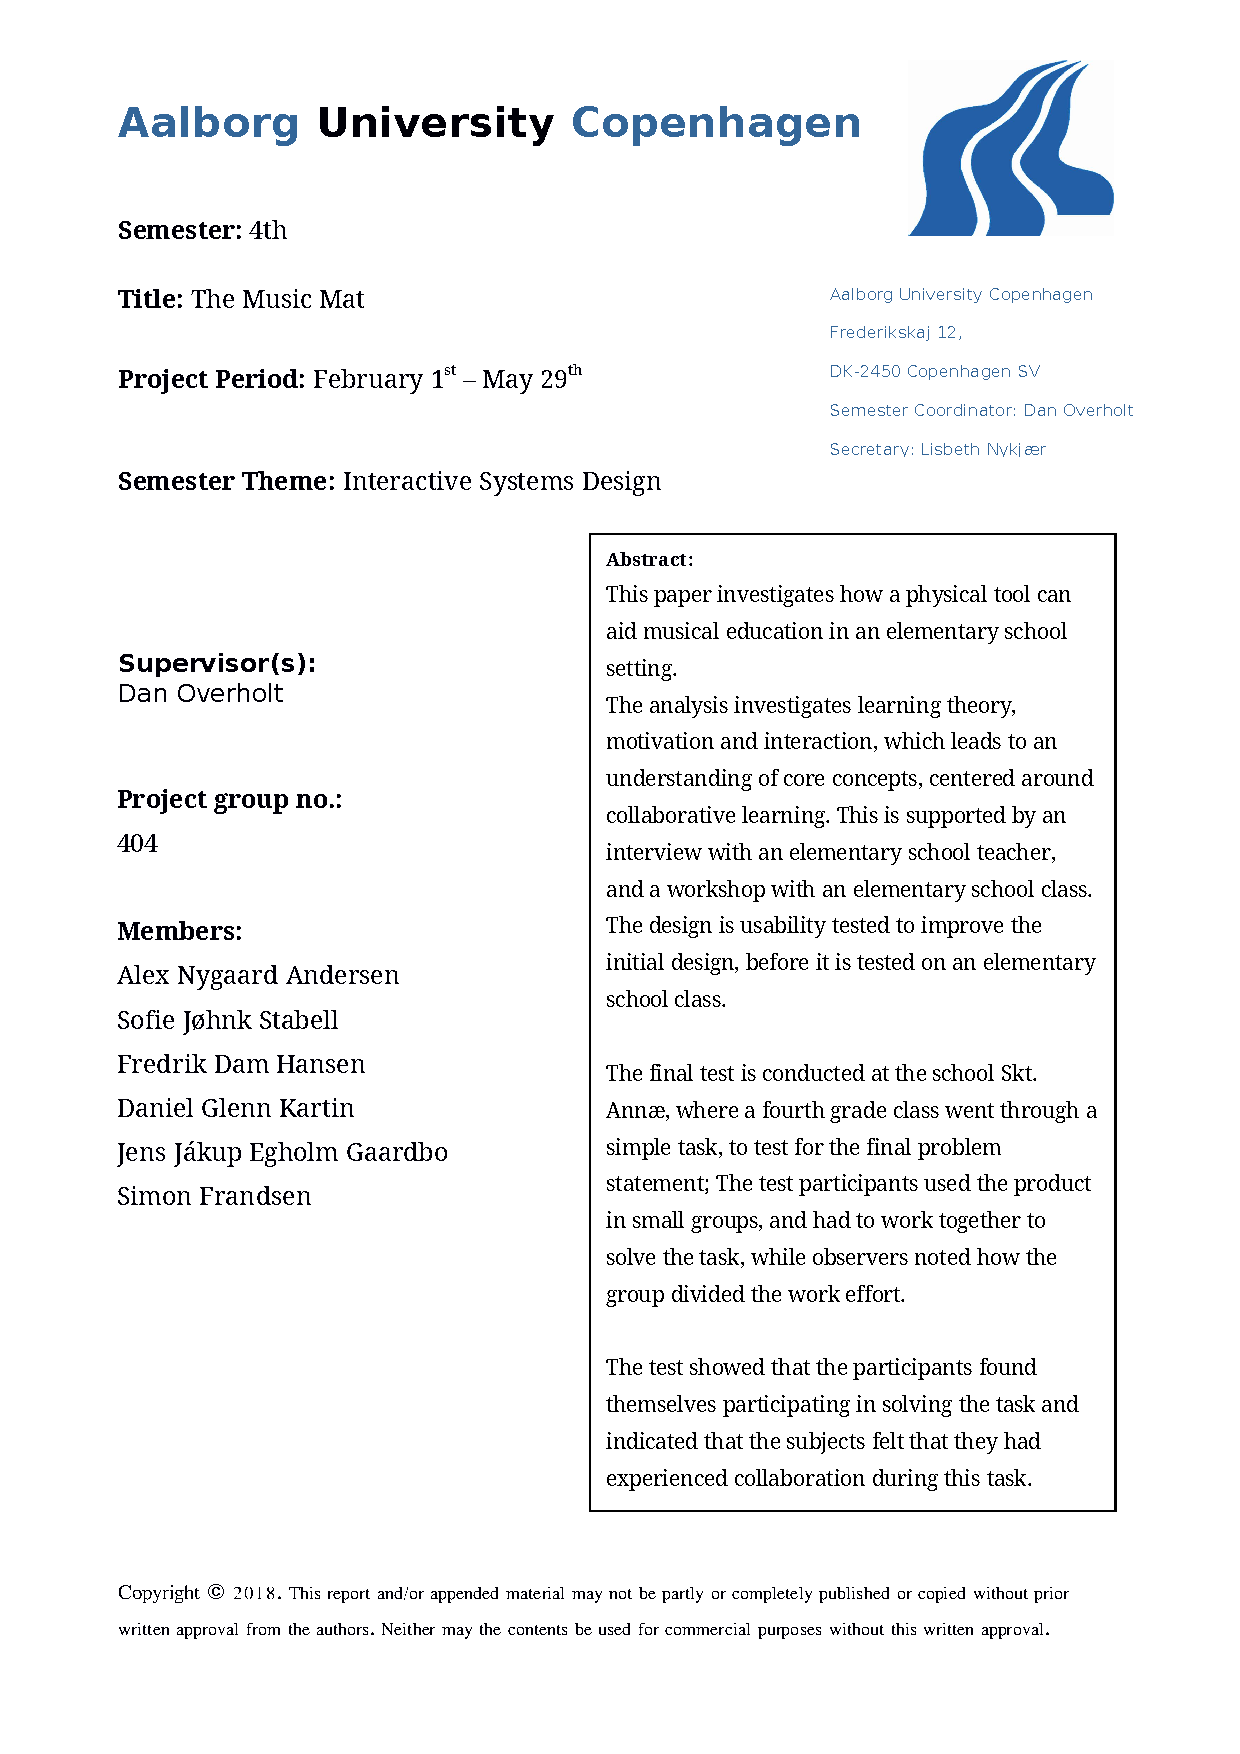
\includepdf[pages=-]{include/frontmatter/Page_0.pdf}

\setlength{\parskip}{0pt}
% INDHOLDSFORTEGNELSE
\tableofcontents

\todo{generelt synes jeg det er rigtig godt, har dog nogle generelle ønsker: 1) HUSK AT LAVE REFERENCER! der er mange afsnit hvor der ikke er en eneste! og mange steder er der for få. husk for hvert udsagn skal der en reference. - også billeder og citater! 2) har nogle ønsker til lidt omrokeringer - interaction skal være det først underpunkt under lærings afsnittet, og FPSen skal rykkes op under "choice of direction" da det er her vi beslutter hvad der skal så i FPSen)}
 
\newpage

\newpage

\setcounter{page}{1} 					% Arabic page numering (starting at 1(one)) throughout the paper
\pagenumbering{arabic}

% INDLEDNING
\chapter{Introduction}
	
	
	

	

% ANALYSE
\chapter{Analysis}
\section{What is music? Audiation:} \todo{Cut from this into the introduction.}
\begin{quote}
	\textit{Sound itself is not music. Sound becomes music through audiation, when, as with language, you translate sounds in your mind and give them meaning.}\\
\end{quote}

Everyone has a meaning about the sound they hear, and the meaning differs from individual to individual. Audiation is the concept of assimilating and comprehending music heard by the individual, either in the present or in the past. We can also audiate through reading notations, composing contemporary music or improvising on an instrument.
The concept of audiation is similar to the concept of language:\\

\begin{quote}
	\textit{"Consider language, speech and thought. Language is the result of the need to communicate. Speech is the way we communicate. Thought is what we communicate. Music, performance and audiation have parallel meanings. Music is the subject of communication. Performance is the vehicle for communication. Audiation is what is communicated."}\\
\end{quote}

An individual can begin audiating shortly after hearing music, to give meaning to the sound. What the individual can take from the audiation depends on that particular individuals previous audiation. The concept is similar to regular conversation – if a group of people are talking, each individual will take their own comprehension of the conversation with them. This comprehension is based on existing knowledge and experience on the topic. 
The concept of audiation increases the chance of remembering what the individual learns long term. Everyone can remember 7 +/- 2 things\todo{Get a reference}, however, if the individual tries to remember something without comprehending it, it quickly slips away again. If students have issues with vocal or instrumental techniques, or they struggle with memory lapses, it is most like due to them not auditing while playing or singing. If the student audiates away from their instrument, it can correct technical and memory issues, including issues related to tone. Audiating before performing sound is key to learning music. Instruments should not be seen as the tool to learn how to understand music, but rather the tool to express the music:\\

\begin{quote}
	\textit{“Just as a calculator becomes a crutch for students who cannot multiply or divide, so music instruments become crutches for students who cannot audiate. This is immediately obvious when students learn to play scales by memorizing fingerings. Although students may recognize they are performing with poor intonation or inaccurate rhythm, their lack of audiation is virtually impossible for them to correct those problem by themselves. Audiation may be expressed through a music instrument, but it cannot be taken from a music instrument.”}\\
\end{quote}

Audiation potential itself cannot be taught but rather depends on how natural musical aptitude comes to the individual. However, while Audition potential cannot be taught, students can be taught how to maximize their music achievement:\\

\begin{quote}
	“By providing children and students with appropriate knowledge and experiences, they can be taught how to audiate, that is, how to use inherent audiation as determined by their music aptitude, to maximize acquired music achievement as determined by the quality of a particular educational environment.”\\
\end{quote}

The issues become evident if the students don’t learn audiation, notation and music theory in the proper sequence, they will be unable to make sense and add meaning the sound and music they hear or the notations they read. It is particularly evident with wind instruments Techniques refer to the methods the teacher uses to teach as well as the tools applied to achieve certain goals in different activities.. If the students are unable to tonally audiate what they see in the notations, but still manipulate the keys or valves on the instrument as the notation instructions, the student will often fall out of tune.
Everyone can learn some degree of music. Similar to how everyone has at least some amount of intelligence, everyone has some amount of music aptitude, so put in other words, everyone is musical. Everyone is capable of learning to listen to and perform music to some extent of success. Generally, two-thirds of humans are average – that includes average music aptitude.
Also it is important to get students of to a good start. The foundation that is created in the early ages is a substantial influence on the music achievement of the student. Most likely, the guidance received in the early stages of their musical careers is a bigger influence, than the guidance the students receive in the higher grades or at colleges and universities. If the students musical skill-set is not properly maintained, they will severely decrease over time.
In order to maintain the skill-set properly, the techniques used by teachers have to be considered as
they are highly important. When it comes to tonation, the rhythm patterns and harmonic patterns are the most prevalent materials and they’ve remained similar for a long time across different nationalities and cultures as they belong to the basics of audiation. On the opposite side, we have activities that include larger classrooms. These will vary a lot depending on the culture, age and experience.\\


\section{Why learn music? The impact of musical education}
Several studies have shown that different types of musical engagement in a variety of ways over a lifespan has an impact on several aspects of personal growth and development. As concluded in the article "The power of music: Its impact on the intellectual, social and personal development of children and young people":\\

\begin{quote}
	\textit{"This overview provides a strong case for the benefits of active engagement with music throughout the lifespan"}\cite{powerOfMusic}\label{quote:powerOfMusic}.\\
\end{quote}

Linguistic abilities and musical training seems to be linked, due to shared brain mechanisms being used to process music and language. Precision in the perception of speech related contrasts, in pitch patterns and other distinctive speech elements have been reported to be associated with musical ability\cite{languageSkills}.\\

A study focused on literary skills showed that a group of second grade students(n = 47) taking piano lessons over a 3-year period had significantly better vocabulary and verbal abilities than a group of control students(n = 57) that did not receive music lessons\cite{vocabularySkills}.\\

Some aspects of mathematical skills have also been shown to be improved by musical training. For example the subdivision process required to read and play from music scores in order to play and keep a rhythm\cite{powerOfMusic}.\\

Other abilities have also been reported to be affected by musical training such as creativity, social and personal development, physical development, health and wellbeing\cite{powerOfMusic}.\\

According to the article \textit{Interactive music video games and children's musical development} there are 5 basic music elements that should be learned in order to get a good understanding and appreciation of music\cite[p.~99]{interactiveMusicVideoGames}:
\begin{itemize}\label{list:basicMusic}
	\item Duration
	\item Pitch
	\item Tone color
	\item Dynamics
	\item Structure\\
\end{itemize}

In another study, which focused on integration of music in the elementary classroom, results were positive. Musical activities activate both the analytical and creative side of the brain, and learning other subjects becomes easier with the addition of a musical element, as the speed at which information is processed increases. An example of this is learning the math of money exchange through music note denotations\cite{musicIntegration}\todo{Is this the cite for the prior claims as well? Cite more through the text and not just at the end.}.\\

Through the initial research, it can be assumed that musical education is important for the development of young students in many facets of life. In order to consider if certain tools can improve the current musical education, an analysis of the study plan applied to the education of elementary school students across Denmark will be analyzed\todo{Maybe write about the section coming just after as well, due to restructure.}.
\section{Learning}
\subsection{Learning Defined}\label{sec:learning}
Learning is the process described as obtaining or modifying knowledge\todo{Where? Cite.}. The ability to learn exists for most living things i.e humans, animals, plants and some machines\todo{Cool, cite.}. \\
\\
There are many types of learning, this report will mainly focus on Active Learning and Passive Learning due to being the main types of learning, when talking about education\todo{Cool, cite.}.

\subsection*{Active Learning}
Active learning comes from a person taking control of their own learning experience. If a student just sits and listens, they will not achieve as much of their learning experience as possible\todo{Cool, cite.}. Active learning comes to play, when the student actively does more than listen. They read, write discuss and engages themselves at the given topic. This also includes doing excersices and solving topic specific problems\cite{activelearning}. The use of active learning in a classroom is vital to improve the learning experience of the students. Furthermore, when not using active learning, up till 70\% of the obtained knowledge is lost within the next 24 hours \cite{learning}.\\

The retention of learning is the concept describing the processed information traveling from the short term memory to the long term memory\todo{Cool, cite.}. Furthermore, retention of learning describes how processed information can be forgotten\todo{Cool, cite.}. As aforementioned attending a lecture without actively participating except listening, can cause a person to lose the majority of information obtained withing 24 hours\todo{Cool, cite.}. Multiple theories within the retention of learning also suggests that the information is not lost, but a person is just unable to recall the information \cite{retention}.
In \autoref{fig:activelearn} the concept of retention of learning is displayed. The figure displays how different ways of learning affects the amount of information learned and remembered. In the bottom bracket, there is the lectures, reading and audiovisual elements. These are the elements which does not actively include the student when obtaining the information, and is therefore the least effective way of learning. In the middle bracket, demonstration, discussion, exercises and play is displayed, these elements provides a hands-on approach to learning and increases the amount of information obtained significantly. This means interaction and taking an active part in solving a problem, will increase the chance of remembering information about the topic. In the top bracket, there is the "learning by doing", aspect containing; working with a coach and practicing is displayed. These aspects are likely to provide the best results. This is because there is a personal approach and the motivation by the student is higher at this point\cite{retention}. 

\begin{figure}[H]
	\centering
	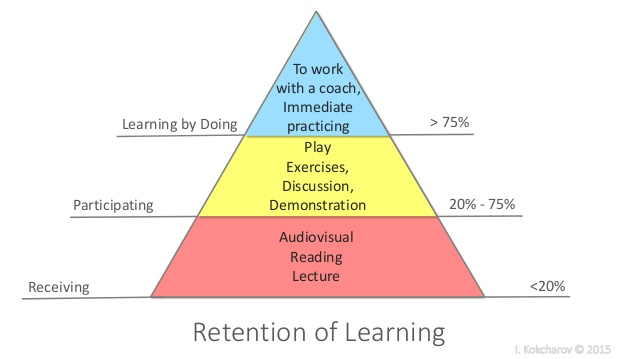
\includegraphics[width=0.9\linewidth]{figure/Analysis/skillslearn}
	\caption{Retention of Learning, taken from \href{https://www.slideshare.net/igorkokcharov/kokcharov-skillpyramid2015}{\color{blue}here}}
	\label{fig:activelearn}
\end{figure}
\todo{Instead of "here" in the caption, we need to add a name, author, webpage or something}
\todo{Also, write caption that describes figure, don't do this in the above text.}

\subsection*{Passive Learning}
Passive learning is teacher-based where the students are not getting involved in the lecture. This form of teaching is usually seen on universities where the professors gives a lecture, and does not provide assignments or feedback to the students. This means that the learning method belongs in the bottom bracket of the retention of learning triangle as seen above. This way of teaching is usually the least efficient when the goal is to teach or alter information\cite{learning}.\\
\\
\subsection*{Sub Conclusion}
When learning is the goal in an education environment, both active learning and passive learning are being utilized. Based on the findings, active learning will provide a better learning experience where the student will be able to remember more information if done correctly. This means that participation and practice as well as motivation and interaction are essential to optimize the learning experience the most.

\subsection{Collaborative learning}\label{collabLearning}

Seen though a biological perspective, humans are social animals\cite{laeringIPraksis}. This has a high influence on the process of learning, since humans as pack animals learn with and from each other - meaning that the learning process is social\cite{laeringIPraksis}. Working in groups and/or teaching each other, therefore strongly appeals to the human brain, and can be considered a powerful impacter when learning\cite{laeringIPraksis}.        

There has been a lot of research on collaborative learning in various educational contexts. However, the more artistic educations have been slightly overlooked\cite{collaborativeLearningTeachers}\cite{collaborativeMusicAnalysis}\cite{collaborativeLearningReview}. 
The article \textit{The Experiences of Elementary Music Teachers in a Collaborative Teacher Study Group} states, based on research outside of a musical context, that:\\
\begin{quote}
	\textit{"collaboration can improve learning outcomes if students make a conscious effort to coordinate their efforts and are able to come to a shared conceptual understanding of the problem being solved"}\cite{collaborativeLearningTeachers}.\\
\end{quote}
However, it is not an entirely unexplored area, and studies have shown that musical collaboration stimulates students critical and creative thinking, and rich musical experiences can surface from combining ideas from larger groups are combined\cite{collaborativeLearningTeachers}. 
The article introduces three principles of collaboration, that are based on interviews with three teachers:\\
\begin{enumerate}
	\item Collaboration facilitates student self-expression and independence.
	\item Students who are collaborating share goals. The teacher allows space for or guides students in creating productive student-student interactions.
	\item A teacher collaborating with her students facilitates their movement toward a shared goal. Teacher provides necessary background skills, creates student buy-in for the goal, and then fades away to allow students to take ownership.\\
\end{enumerate}
The first principle is at work when students, for example, are divided into smaller groups, and find themselves focusing on a task that generates communication, arguments and discussions without the teachers involvement. They will show independence as they individually will try to convince others to reach the same conclusions.\\

The second principle is related to a student groups shared motivation while focusing on a shared goal, for example presenting their work for the entire class, and sharing the responsibility to reach that goal.\\

The third principle is a teacher-student collaboration that also can be present withing the classroom. Here the teacher will for example instruct the student with harmonies, rhythms, chord progressions etc. after which the teacher gradually removes him/herself and let the students take control over the task at hand.\\


\subsection*{Sub conclusion}
Collaborative learning lies in the human nature and can be considered as a great and positive influence in the learning process. Furthermore is has an impact on various aspects of personal development such as a positive impact on creativity, musical influence and social interactions that could potentially be very useful later in life.


\subsection{Interaction in a learning perspective}
As mentioned in chapter \ref{sec:learning} a hands-on approach and interaction is important to get an efficient learning experience. This chapter will focus and go in depth interaction in correlation to learning.\\
\\
First of, interaction is the description of the occurrence when objects er people interacts with each other, this can be a person interacting with an object, or an object interacting with another object etc.\\
\\
As mentioned, it is important that the students and the teachers are actively involved in the learning activities to achieve as much as possible from their learning experience. First, students should have an opportunity to interact with teachers as well as the other students, to increase their learning opportunities. Secondly, the teacher should provide a classroom with room for involvement and motivation in the learning process\cite{interactionlearning}.\\
\\
A different view of interaction in a learning perspective is not only the interaction between students and teachers, but also a hands on approach for the students when learning about new subjects. This is also refernced to as Kinesthetic learning or tactile learning. Kinesthetic learning is what describes a student carrying out physical activities rather than rather than listening passively to a lecture. This learning by doing approach is among the most popular learning methods among the students. This method gives the students space to experiment with trial and error as well as learn from their mistakes.\cite{kinest} \\
\\
{\color{red}When trying to understand music in an interactive sense, one might look at another medium that incorporates interactivity: video games. In particular, one could look at interactive video games that focuses on playing or teaching music. Lily Gower and Janet McDowall conducted a study, in 2012, centered around the educational qualities gained from playing such interactive music video games\cite{interactiveMusicVideoGames}. The study aimed to establish if interactive music video games had an educational value when integrated into the existing music education.\\

The different games mentioned in the study were Guitar hero (See \autoref{sec:guitarHero}), SingStar and Wii Music. What these games have in common is that they all use interactivity as a means to playing music, be it with a guitar shaped controller, a microphone or the Wii remote held like an instrument. These games try to emulate what it would \textit{feel like} to play a guitar, sing or play different instruments.\\

The study interviewed two music teachers of different musical abilities, and 9 music students aged 11-14 (5 male and 4 female) from different socio-economic situations. The student participants came into the study with different levels of musical experience. The interviews were semi-structured of nature to allow free flowing conversation. Interviews with the children participants revolved around their prior music backgrounds and past experiences with interactive music video games. The interviews with the teacher participants discussed their personal views and experiences with interactive music video games, like Guitar hero (\autoref{sec:guitarHero}), in relation to music education.\\

Teacher two said during the interview that:
\begin{quote}
	\textit{"...the whole debate about whether it’s music making, that’s a whole other debate, but whether it’s developing some across the board generic skills, I’d say yes."}\cite[p.~98]{interactiveMusicVideoGames}.\\
\end{quote}
Meaning a belief in interactive music video games giving the students some educational values in a more general music setting. In addition, when asked about coordination benefits, Teacher two said the following:
\begin{quote}
	\textit{"...To play at the higher levels of that game [Guitar Hero] requires very high level coordination skills and you’re coordinating visually with what you’re playing as an instrument. So it’s not so different I think physiologically from what a musician does anyway which is to respond to a conductor visually, respond to the music score visually, and then play accordingly to a set tempo, and timing is everything. So, the game is about scoring high scores all based on your capacity to play in time on the right note and what’s that sound like? Sounds like music playing to me."}\cite[p.~98]{interactiveMusicVideoGames}.\\
\end{quote}
Teacher two has a firm belief that Guitar hero specifically has a high coordination requirement, and thus to play at the higher difficulty levels of the game, you need good eye-hand coordination, which he thinks correlates in a physiological way directly to the way real music is played.\\

When the student participants where asked about their musical knowledge gained from playing interactive music video games, one girl said:
\begin{quote}
	\textit{"Yeah, so it’s like you find out about more songs that you don’t know about . . . there’s a lot of songs that you don’t know about and then you like listen to them and then you get into either like the artist or the type of songs or you just listen to that song and stuff and then you go looking on the net for other songs of that type and stuff, so it opens up a whole lot of stuff."}\cite[p.~100]{interactiveMusicVideoGames}.\\
\end{quote}	
The participant felt that she had gained music knowledge, and broadened her musical identity. The exposure to the new music, gave her an interest in new artists and genres she might not have known about.\\

The discussion about whether or not interactive music video games provide the children with a basic understanding of essential musical elements, is argued by Lily Gower and Janet McDowalls, to be that they at least learned about pitch and rhythm, while maybe not the rest of the five elements seen in \autoref{list:basicMusic}. Meaning the interactive music video games assisted the children in Lily Gower and Janet McDowall's study develop some basic music skills, that might correlate to real music making\cite[p.~99]{interactiveMusicVideoGames}, and potentially could assist other children in similar age groups.

\subsubsection*{Sub conclusion}
In conclusion, the children in the study\cite{interactiveMusicVideoGames} did seem to learn at least two basic musical elements from interactive music video games, being pitch and rhythm. In addition the children also felt they had gained musical knowledge from these games. Hence interactivity in musical education, it being from Guitar Hero, SingStar or another interactive music medium, seems to assist children in development of some aspects of musical abilities.
}\todo{This part is not "Officially" part of interaction but still seems relevant, read through the chapter and see if it fits somewhere else}
\subsection{Movement in a learning perspective}
	\todo{Write about John Ratey and Spark.}
	\cite{kinestheticMovement}
\subsection{Motivation theory}
Motivation is an integral part to learning\cite{motivationGameDesign}, and is therefore important when looking at ways to assist children in learning music. The most fundamental motivational theory is the one called Self determination theory (SDT)\cite{SDT}. SDT proposes that motivation is divided into two brackets; Intrinsic motivation and extrinsic motivation\cite{SDT}. 

\subsection*{Intrinsic motivation}
Intrinsic motivation is the internal motivation, that pushes humans to do actions not depending on a specific reward, but wholly depending on the inner need to do the action, for the sake of it\cite{SDT}.
This is the inherent need humans have to learn, explore and widen their knowledge\cite{SDT}.\\

To establish what influences intrinsic motivation, the researchers behind SDT\cite{SDT} created Cognitive evaluation theory(CET) as a sub-theory within the existing SDT. CET is the theory that focuses on competence and autonomy in relation to intrinsic motivation. The first part of the theory says that social-contextual events that contribute to the feeling of competence for a performed action, improve the feeling of intrinsic motivation in relation to that action\cite[p.~70]{SDT}. These social-contextual events might include rewards, feedback and communications\cite[p.~70]{SDT}. For intrinsic motivation to be improved, the action that is performed must be accompanied by a feeling of autonomy\cite[p.~70]{SDT}.

\subsection*{Extrinsic motivation}
Extrinsic motivation is the motivation that drives a person, depending on a reward associated with the performed action. From the SDT theory extrinsic motivation is defined as: 
\begin{quote}
	\textit{The term extrinsic motivation refers to the performance of an activity in order to attain some separable outcome and, thus}\cite[p.~71]{SDT}.\\
\end{quote}
An extrinsically motivated action could be; performing a non enjoyable job, meaning that there is no intrinsic motivation to the work, but when a paycheck is introduced, the action would be extrinsically motivated.

\subsection*{Emotions}
Emotions and motivation have a sort of bidirectional relationship in which each side can activate or deactivate the other\cite[pp.~66]{emotionsAndMotivation}. In addition to that, emotions directly impact the quality of learning\cite[pp.~66]{emotionsAndMotivation}. In the book\cite{emotionsAndMotivation}, they use an example with a student named Jake, he has had past negative experiences with studying. This later deactivated his motivation to study in the future, because the negative emotions relating to the bad experience interrupted his goal of studying\cite[pp.~67]{emotionsAndMotivation}. To better counter the negative emotions, and deactivation of motivation, one must consider highlighting the intrinsic task value of an action\cite[pp.68]{emotionsAndMotivation}.

\subsection*{Sub conclusion}
In conclusion, whether motivation is extrinsic or intrinsic, it is a core part of performing any action. Thinking about learning specifically, the intrinsic task value should be considered to be highlighted, so as to counter negative emotions.\todo{Put more weight on positive/negative emotions, in terms of motivation.}

\section{How is music taught? The Study plan}

According to the study plan, found on the website of the Danish Ministry of Education(Site) the children are required to learn three areas of competence. Within these are musical performance, musical creation and musical understanding.

\subsection*{Musical performance}
Musical performance includes teachings about singing, movement and playing instruments. More specifically teaching the children about how to sing individually and in groups, as well as teaching them about different kinds of singing and songs. Furthermore, teaching the children about movement in a musical context, such as dancing and rhythmic movement. Finally, being able to play the basics of different instruments, such as drums, guitar, piano or keyboard and different wind instruments.

\subsection*{Musical Creation}
Musical creation includes the teachings of different abilities in relation to create, alternate or improvise musical pieces. The children should be able to compose music with the ability to remember time and tempo when creating music. Furthermore, the children should be able to form and shape sound into something rhythmic. Besides creating music, the children should also be able to change music with the help of adding sounds, or changing the pitch or pace of sound. Finally, the children should be able to improvise music without being given a specific assignment to follow.

\subsection*{Musical Understanding}
Musical understanding is, first of, to be able to express music in other forms than sound. For an example, they should be able to express themselves verbally about music and be able to draw music. The children should have knowledge about instruments, and the ability to distinguish the different instruments from their appearance as well as their sound. The children should be able recognize specific elements in a musical piece and identify them. Finally, they should have the knowledge of musical history, in relation to different music genres as well as music from different time periods.
\\

When the children get older, they will be introduced to digital tools and synthesizers to be used in the classroom. These tools might include iPad or Garageband. On these devices, they are asked to compose a musical piece using the aforementioned knowledge.\\
In the lower grades, the children are working more with analog instruments as well as singing to develop a musical foundation for their education.
\\

The study plan opens for a broad interpretation of elements that are taught and with which tools this knowledge gets taught. After analyzing the study plan, it became evident that an interview with a teacher is necessary to get a profound understanding of how the course “Music” is taught in elementary schools.\\

\section{Problem Area}
As this report will try to improve current tools in modern musical education, it is important to understand how the current education functions. In order to establish a target group, the current musical education in elementary schools will be analyzed. Firstly, an interview with a music teacher at an elementary school will be conducted, to clarify issues with the current education. \\	



\subsection{Interview with Hanna Jørgensen}
Hanna Jørgensen is a teacher in music at both elementary school level and Danish Gymnasium level at Sankt Annæ Skole. She is also a pedagogue in Musical Pedagogy at the National Music Conservatory. Besides the aforementioned credentials, she is also involved in “Børne og Ungdoms Forvaltningen”, which is an organization that tries to improve the quality of life among children and young people. She is interviewed to help establish a detailed view on how the current musical education functions, and to help locate issues within the musical curriculum for elementary school children.
The interview with Hanna was conducted at Sankt Annæ Skole and was established to clarify how the current education functions in practice, and which issues are present in her opinion.\\

The beginning of the interview focusses on the current structure and tools used in the education. Hanna explains that the current study plan, for her class, is divided into clear courses with focuses on a particular subject. A few elements are consistent for the courses, in the way she teaches. Games and movement are two tools that are fundamental for how music is taught in elementary school. There are currently a set of tools used to teach music through games, she does however see a lack of general tools, and there is definite room for innovative ideas.\\

She also emphasizes the importance of Rhythm. Rhythm is a specific important thing that the children are taught. It is essential for singing, playing instruments and understanding music. This means that a focus is on the learning and understanding rhythm in elementary schools. The children mainly use singing as a tool for learning. Instruments are not used as commonly, as they are harder to get by and singing provides a tool that everyone possess, in order to learn rhythm. When it comes to the theoretical education, Hanna finds it essential to work with visual and physical tools. Currently, she uses a carpet with note lines drawn on it, as it is a physical tool and she can get the kids to collaborate when creating and understanding music. The collaboration is another theme, that Hanna finds important to teach the kids, however she finds a lack of tools currently. The class that Hanna teaches uses PC Software such as Garageband, but the interface is limited to a single user at a time. She is seeking physical tools that allows for creative thinking when collaborating. \\

Hanna is very clear, when she says that the children have an easier time learning, when working with physical objects. Another tool that Hanna uses in her class are Lego blocks, which is a small tool that can be used in various ways. She uses it to explain steps in music. She is very fond of the idea of physical blocks that can be used in versatile ways.
Hanna ends with the conclusion that the biggest issues she has currently, are physical tools that can be used collaboratively between her students.\\


\subsection{Workshop}
In order to get a closer look at the students learning music, a workshop was established at Sankt Annæ Skole. The workshop was created in collaboration with Hanna Jørgensen, who teaches a 4th grade class in music at Sankt Annæ Skole.\\

The goal of the workshop was to get an idea of what the children thought about their current music education, what tools they use and how these tools could be improved. The children were presented with different ideas for new and alternative tools that can be used in the education. They had to provide feedback on the ideas and compare them to existing ideas, to find what elements of the different tools the students themselves desires.\\

Across the different ideas in the workshop, a number of themes became apparent. The following points were the most prominent when it came to desired features:\\


\begin{itemize}
	\item[-] \textbf{Movement}\\
	The students found the current education to be very still. They desired ways to be more active and have more movement as part of the education.\\
	\item[-] \textbf{Variation:}\\
	The students made it clear that they dislike using the same tools and same methods for learning various aspects. Having variation to keep things fresh would be more fun.\\
	\item[-] \textbf{Games:}\\
	The students love to learn through games. They feel like they remember a lot of what they learn, when they use games and they have fun while learning. \\
	\item[-] \textbf{Visuality:}\\
	The students asked for more visual components in their education. It is important to them that what they use are presented in front of them visually and had colors that were pleasing to look at.\\
	\item[-] \textbf{Physical:}\\
	The students, in extension of components being visual, loves when the tools are physical. If they can see, touch and feel the objects they use to learn, they have more fun and feel like they learn.\\
	\item[-] \textbf{Group work:}\\
	The students expressed great joy about working together with their classmates and collaborating in different ways about creating and understanding music.\\
	
\end{itemize}



\subsection{Target Group}
Based on the knowledge gained about different learning theory, current tools used in education, an analysis of how the current education is and how the students perceive it, the target group will now be presented.
The target group for this project are children aged 8-12, currently residing in elementary school and participates in the course “Music”.\\

The findings display a great potential to provide a tool for these students.
Furthermore, the teachers of the course “Music” will be considered a sub target group for the project, as the tool this project aims to provide would have to be used and explained by the teacher. The teacher would have to use the tool to provide knowledge and add meaning to what the tool represents.
 
 
\subsection{Learning tools used}%Mini SOTA
This section is about the learning tools that the target group have been using in classrooms. It concentrates on music material used in schools and what Hanna from Sankt Annæ uses for helping her students understand music notation and music theory. 

\subsubsection{Garage Band}
Garage band is a software developed by Apple, Inc. It is used for allowing users to create, editing and rendering music. The whole idea about Garage band is that the software uses pre-made MIDI keyboards, loops and arrays of different instrumental effects and voice recordings that can help the user further develop various sounds. This software is a very helpful tool for learning how to create music.
\begin{figure}[H]
	\centering
	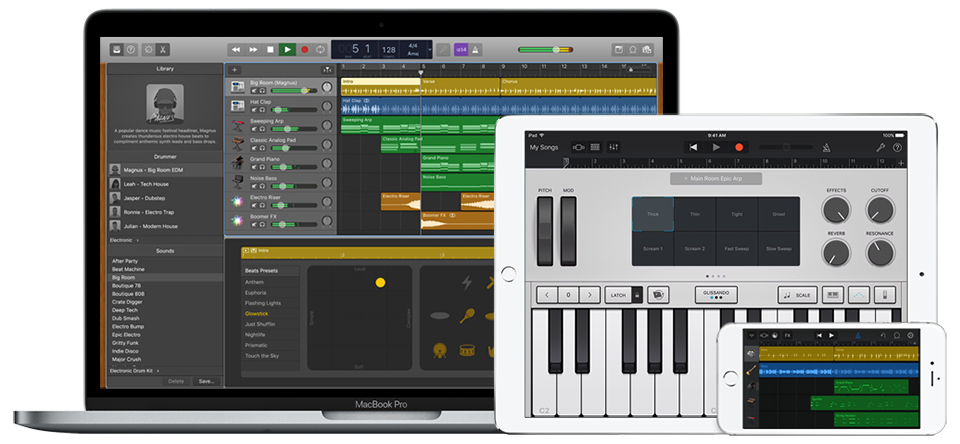
\includegraphics[width=0.7\linewidth]{figure/Analysis/garageband}
	\label{fig:garageband}
	\caption{Garage band}
	
\end{figure}

\subsubsection{Lego - Music notation}
Lego is a variance of physical plastic blocks that are used for building a variety of designs. They come in different lengths and designs and the idea is to build whatever the individual desire. Electronic components like motors, LED lights etc. have been made for adding more control and innovation for the individual creator. The usefulness of Lego is the capability of using it for anything creative such as understanding music theory. 

\begin{figure}[H]
	\centering
	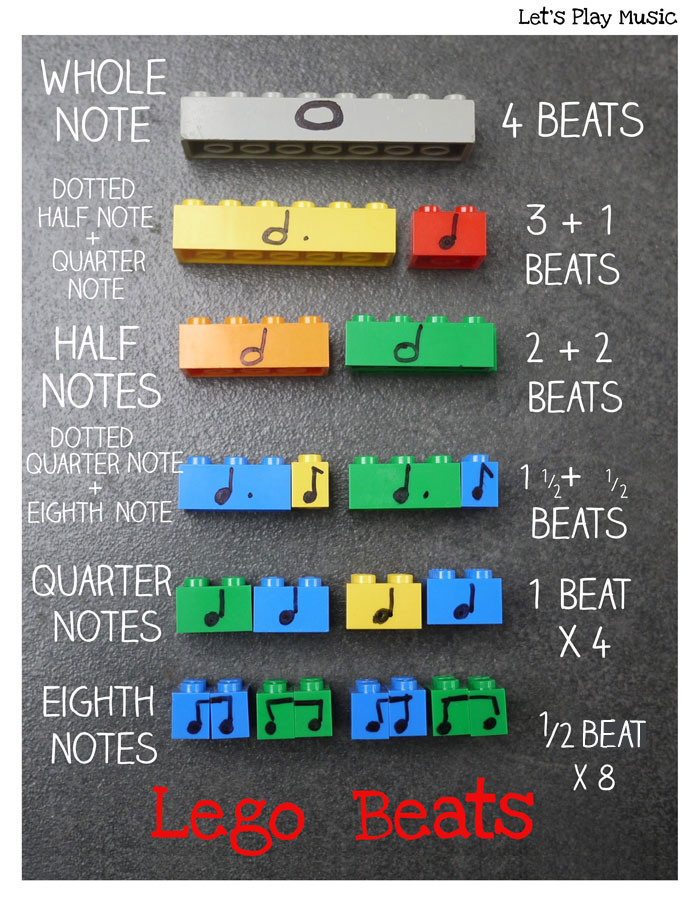
\includegraphics[width=0.7\linewidth]{figure/Analysis/lego}
	\label{fig:lego}
	\caption{An example of how lego could be used for Music notation}
\end{figure}

\subsubsection{MuseScore}
MuseScore is an open-source software program for creating music notation. The main attraction of the software is the ability to play and practise sheet music anywhere. You are able to search for new music sheets and practice thsese by either listening to the notes or change the notation. It is available for windows, mac, IOS, Android and Kindle Fire. It has an input via MIDI keyboard and can transfer to and from other programs via MusicXML, MIDI etc. This is a very useful tool for understanding music notation and practice it hands on. This software is a good example on learning notation for beginners to expert or just experts that want to create music. The program is build so that anyone wanting to create music can. MuseScore also provides their own definite guide to MuseScore. In contrast to many other softwares that lets one build notation sheets, this specific software is free. 

\begin{figure}[H]
	\centering
	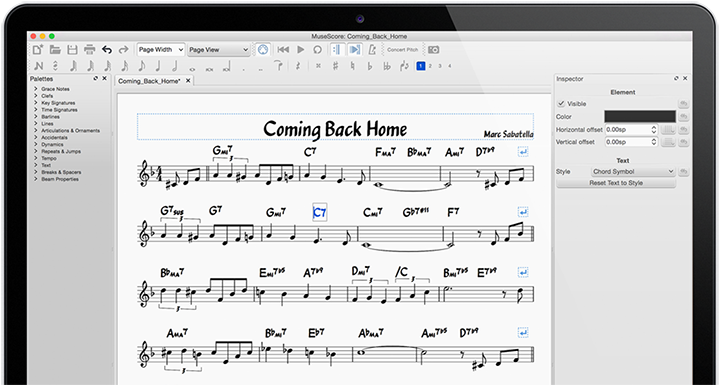
\includegraphics[width=0.8\linewidth]{figure/Analysis/musescore.png}
	\label{fig:MuseScore}
	\caption{MuseScore}
	\href{https://musescore.org/da}{\color{blue}here}
\end{figure}

\subsubsection{Go Fish - Music notation}
Go fish is a card game played by two or more players. The rules state that five to seven cards are given from a standard 52-card deck to each player. The remaining cards are spread out on a table. When it is a players turn, that player can ask any other players if they have the same card value (this means the same number value). If they do, that card is given to the player that asked and if they don’t the player is asked to “go fish” which means the player who asked has to pick a card from the pile of cards on the table. The idea for winning is then to gather as many sets of cards of the same value. This game can be used for many other purposes than using the standard game of go fish with a standard 52-card deck. Hanna from Sankt Annæ is playing this game with her students where she do not use the standard 52-card deck but uses cards with music notation. Making it a learning tool for people trying to memorize or learning the different notations of music. 

\begin{figure}[H]
	\centering
	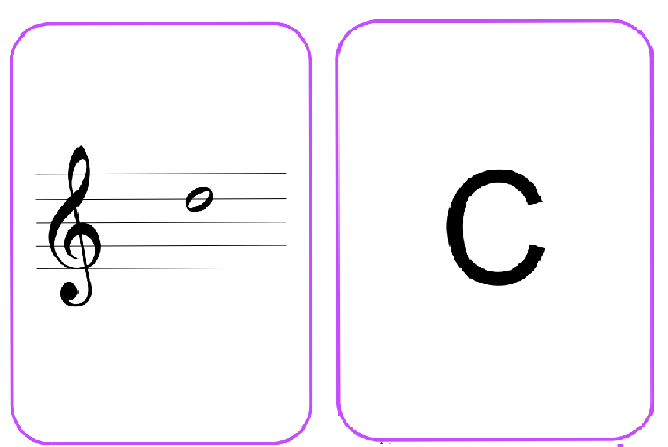
\includegraphics[width=0.7\linewidth]{figure/Analysis/gofish}
	\label{fig:gofish}
	\caption{Go fish example with notes}
\end{figure}

\subsubsection{Sibelius}
Sibelius is a software program for creating music notation. It was created by Sibelius Software. The software can edit, print, play the music using synthesized sounds, produce scores and public scores for others via the internet. The software supports all music notation as well as the most complex notation to produce. It can be used for playing the music or turning it into MIDI or either audio files. It supports basically any MIDI device and it also comes with some pre-made sample files. It also uses third party plug ins such as Vienna Symphonic Library or Mark of the Unicorn’s symphonic instrument.  

\begin{figure}[H]
	\centering
	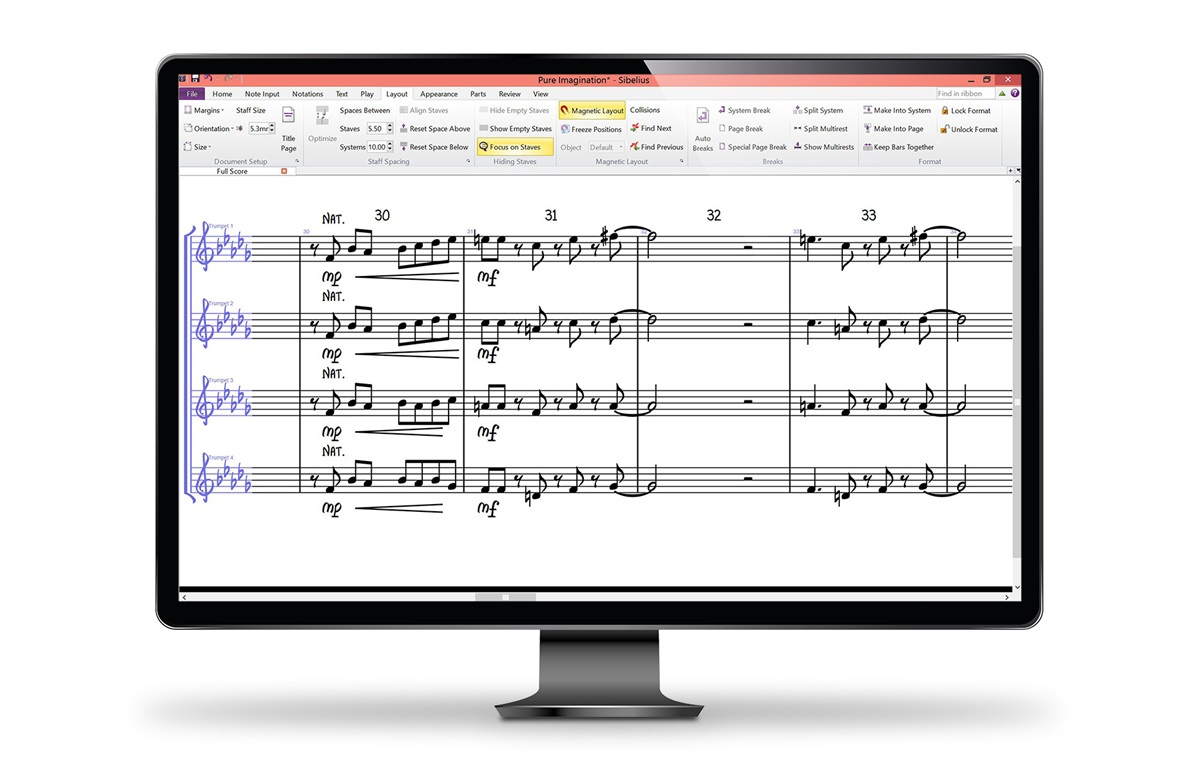
\includegraphics[width=0.7\linewidth]{figure/Analysis/Sibelius}
	\label{fig:sibelius}
	\caption{Sibelius}
\end{figure}

\subsubsection{Clio Online}
Clio Online is an online tool for students who wants to learn more about the different topic provided in high school. You can learn topics such as Danish, English, German, religion, history, biology, sports, music, arts, food etc. This is a tool used by teachers to help their students with their studies. 

\subsubsection{Music work out}
Music work out is a tool set developed by Anette Præst Nielsen. It is a box consisting of different games or teaching methods for users who want to learn or have fun with music. There are currently two different editions – A teacher’s edition and a Game edition.  The Teacher’s edition contains: Around 800 cards and accessories. It is used for learning about theory, notes- and ear training, rhythm cards, interval cards, rest cards, time signature cards, solmization cards, subdivision cards, clef card etc. The game edition contains: 3 different games – Domino, bingo and memory. Which also consist of different parts of the above topics. 

\begin{figure}[H]
	\centering
	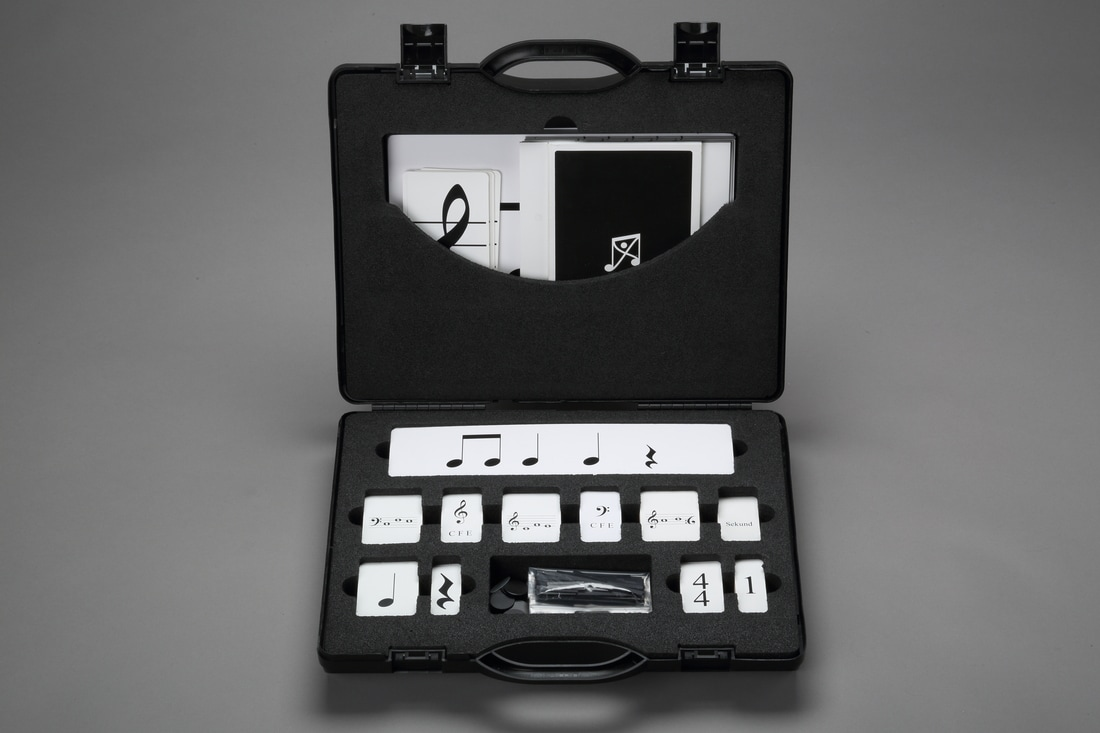
\includegraphics[width=0.7\linewidth]{figure/Analysis/musicworkout}
	\label{fig:musicworkout}
	\caption{Music work out}
\end{figure}

\subsubsection{Music mind game}
Music mind game is developed by Michiko Yurko. It is physical games providing alphabet cards, blue jello sticks and bingo cards. The various subject areas that can be bought are dictation and sight signing, alphabet and intervals, reading rhythms, rhythm math, staff and notes, tempos, music symbols, scales and key signatures, triad and chords. All these games are great learning material for teaching children music. 

\subsubsection{Little bits}
Little bits are different bits of electronic components that can be connected to each other to created different interactive designs. Each module is an electronic circuit and each of the modules comes in four different colors. Blue is for power, pink is for input, green is for output and orange is the connector. This is for learning children about circuits, innovation and how each component functions in a very low level environment. 

\begin{figure}[H]
	\centering
	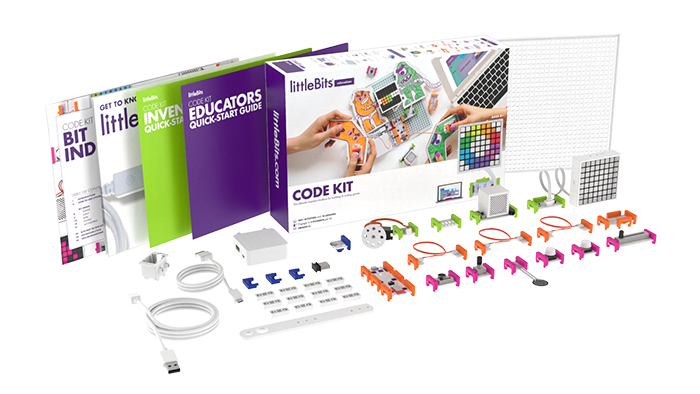
\includegraphics[width=0.7\linewidth]{figure/Analysis/littlebits}
	\label{fig:littlebits}
	\caption{Little bits}
\end{figure}
  
\subsection{Choice of Direction}
The knowledge gained in the problem area chapter, provides a direction for the progress of the project. A look at the study plan gives an overview of how the schools currently teach music through the three areas of competence; Musical Creation, Musical Knowledge and Muiscal Performance. An elaborated interview with Hanna Jørgensen provides insight in current issues with the musical education, which leads to an analysis of the potential target group. This helps establish the target group of 8-12 years old.\\

With the target group established, an analysis of the tools currently used by the target group, in the context of the information gathered through the interview and workshop, highlights issues with a lack of physical tools that the target group can use to learn music in collaboration with each other. Both Hanna Jørgensen and the children asked in the workshop expressed issues with the lack of tools, that can be used when working in groups, while being a physical tool, that the students can touch and have visually presented in front of them.\\

With the knowledge gained in the initial analysis and regarding the study plan, the project will aim to focus on the aspects of musical creation, as the workshop displayed that the target group expressed a need for new tools to learn elements of this specific area of competence.
The following analysis will focus on the aspects found in the problem area. Collaboration and how working in groups affect learning will be researched, to gain a broader understanding of how a product could be developed, that fills the requirements of the target group.\\





\section{Working in groups - different aspects and approaches} % Sofie (sammenflet)

When working in groups different aspects affect the productivity and level of performance \cite{GodKlassekultur} and thereby affects the learning outcome for both the group and individuals. in this section some of these aspects will be discussed. These include: The arrangement of groups, the teachers role, roles within a group, inclusion and exclusion from a group, Feedback as an important group tool, and different collaborative learning Methods - collaborative-, competitive-, and peer Learning.

\subsection{The arrangement of groups}\label{GroupArrangement}
Practical issues such as arranging tables in rows does not promote ideal group work but is more useful when a teacher is speaking to entire classes\cite{collaborationSocialPedagogy}. A more flexible table arrangement is more preferable, as it can be customized to fit the work process and group size\cite{collaborationSocialPedagogy}. 

The number and sizes of the groups need to be taken into account and correspond to the total number of students and teachers within the class. Assuming that there is a classroom with 32 students a grouping of 4 students in each group will mean that a teacher needs to prepare and manage 8 groups which can be more difficult. Fewer larger groups with more members, 6-8 pupils, however, will be more convenient for a teacher to manage, but the learning outcome of the individual students within the group might not be ideal\cite{collaborationSocialPedagogy}.\\


\subsection{The roles within a group}
Group stability and dynamics are other factors that teachers might need to consider. It might be more beneficial for the students to be arranged in groups based on the teachers prior knowledge about the students' behavior and stick to the same groups for longer periods\cite{collaborationSocialPedagogy}, as this gives the group time to challenge the knowledge in the group, and learn the members differences and thereby gain understanding of the importance of different work approaches and processes\cite{laeringIPraksis}.

Differences among people when working in groups are important, as the group members then contributes in different areas (both academically and social), and can thereby overlap each others strengths and weaknesses \cite{ProjektarbejdesKompleksitet}. These individual collaborative roles (based on Belbins team roles \cite{ProjektarbejdesKompleksitet}) can be categorized in three main categories: 
\begin{itemize}
	\item[-] The thinking role - focus is, being creative making ideas, and the outcome of the work. 
	\item[-] The doing role - the focus is the process of the work (how and why)
	\item[-] The social role - focus is the wellbeing of the group. 
\end{itemize}

Having a representative from each category strengthens the group work and outcome thereof - and thereby the learning outcome\cite{ProjektarbejdesKompleksitet}. However if not represented and/or the importance of each role is not acknowledged, it can led to conflicts within the group. These conflicts, can often be seen as difficulties within certain areas (eg. problems with organizing, leading to unstructured work), or the feeling (and expression) of a not equal contribution, which can lead to social conflicts (which in some cases leads to exclusion from the group)\cite{ProjektarbejdesKompleksitet}. 

\subsection{Social inclusion and exclusion}
Being a part of a community/group lies to human nature and is important for the individuals wellbeing  \cite{ProjektarbejdesKompleksitet}- thereby also their motivation, and can therefore effect the learning process. Being excluded from a group has a negative effect on the individuals learning and social wellbeing. This can even influence the person being excluded to avoid future group work due to the psychological defeat. The Danish professor in social psychology Dorte Marie Søndergaard, calls this \textit{social exclusion anxiety} \cite{ProjektarbejdesKompleksitet}. Being excluded is often related to the contributions (or lack of same) value. If the group members contribution does not meet the requirements or is seen as of less value, exclusion can occur. Exclusion can also be caused by character traits and personality, and might therefore not necessarily origin from academically reasons \cite{ProjektarbejdesKompleksitet}.
To reduce the risk of exclusion (and facilitate inclusion), the group must function socially and (as mentioned ) understand the importance of the different collaborative roles. The tasks that groups need to complete have to be designed in such a way that encourages collaboration and discussion and not promote individual work in order to produce an effective learning outcome \cite{collaborationSocialPedagogy}. To further enhance inclusion, the tool of Feedback can be used. 


\subsection{Feedback}
Feedback given between members of the group, is a highly important part of group work\cite{laeringIPraksis}\cite{ProjektarbejdesKompleksitet}. It is with this tool that the group can reflect on their work, and together work towards a joined goal, improving the learning process and outcome for both group and individuals\cite{laeringIPraksis}\cite{ProjektarbejdesKompleksitet}. It is also a tool which can be used to acknowledge each others work, and enhance inclusion and social wellbeing\cite{laeringIPraksis}\cite{ProjektarbejdesKompleksitet}. 


\subsection{Collaborative learning Methods} 
When collaborating, the process and methods must relate to the type of work/assignment. Collaboration can therefore be conducted in many ways. In the following sections three acknowledged collaborative methods, namely \textit{ Cooperative Learning, Constructive Competition, and Peer Learning}, will be discussed.  

\subsubsection{Cooperative learning}
A term which is used widely within the umbrella term collaborative learning(see \autoref{collabLearning}) is cooperation\cite{collaborationCooperation}. It is a teaching strategy in which children in smaller groups in a class room cooperate towards a common goal and thereby develop their social skills whilst building a common base of knowledge about a course subject\cite{collaborativeLearningTeachers}\cite[p.~15]{peerLearning}\cite{collaborationCompetition}. Even though cooperative learning has shown positive results in learning outcomes of pupils, it has also been critisized. For example because there in some cases will be students taking on most of the work, while others do nothing. It is also critizised for the risk of it causing competition between either group members or whole groups\cite{collaborationCooperation}.

\subsubsection{Constructive Competition}
Competition tends to be seen as a negative and destructive force when talked about in a learning context and is often conceptiualized as an opposite to collaboration. However, in the right conditions it can be constructive as it is simultaneously a strong motivator\cite{collaborationCompetition}. %Den her skal nok uddybes en smule

\subsubsection{Peer Learning} %Sofie
In Peer Learning, equal individuals (eg two students) (non professional) work together (in peers) to archive their individual goals \cite{peerLearning} - often in a "tutor/mentor"-"tutee/mentee" relationship. The idea is, that though mutual help and support, knowledge should be shared between them, as so the goals will be to either learn by teaching or by being tough. This can be done in different constellations\cite{collaborationCompetition}.

\begin{description}
	\item[Peer Instruction] The students meets prepared in given subject, the teacher asks a question in the subject, and the individuals state their answers. Next, the assigned peers discuss the question and based on this, state their reevaluated answers. In this process the students have prepared themselves in the same material, and so their knowledge might not vary significantly, and the roles of tutor and tutee might not be present.  
	
	\item[Peer Tutoring] Each of the peers must prepare and be able to teach individual given material, to the other peer. The peers is therefore in the roles of \textit{Tutor} and \textit{Tutee}, and shifts roles after a certain amount of time. This process relies on the fact that each of the peers have a greater understanding in a subject than the other, as the roles of tutor and tutee will become present.     

	\item[Peer Mentoring] This resemble the process of Peer Tutoring, but instead the students must have different skill and experience level (eg. comes from two different grades). Instead of a tutor and tutee, the terms \textit{Mentor} and \textit{mentee} is often used, as the social relationship is often more in focus than achieving academically skills.      
\end{description}   

For all different approaches to Peer Learning it applies that, the teacher must have a deep understanding of the individual students, both in terms of social and professional skills \cite{collaborationCompetition}. Otherwise the Peers might not have the right prerequisites for the collaboration.
Furthermore as Peer learning revolves around the will to share knowledge, the Peers approach to the process is crucial for the success of the process\cite{collaborationCompetition}.


\subsection{sub conclusion} %Sofie og Jens
Understanding how the teacher should (preferably) form groups, and how the dynamics of the group members effects the work, will help in understanding how the tool of this project should strive to relate and support both these arrangements and collaborative roles. The purpose of this focus should be inclusion, and thereby a higher learning outcome for both the group and individually. 
When having this focus, the collaborative methods can act as guidelines for the design and usage of the tool. 

As most the factors concerning group forming, dynamics, and arrangements,  will be in the hands of the teaches, they might not be something that can be directly designed for.  
However, based on the sections founds, it was found most suitable, if the tool could be used for groups of the size 2-6 students and should rely on a flexible seating arrangement.
 

\section{The classroom environment -understanding the context} %Jens


\section{State of the art - Design Inspiration}\label{sec:sota}
In this section of State of the art the focus will be on the design inspiration conducted from the analysis. This will be the inspiration for development design requirements and design. It will provide aspect from physical interfaces to digital interfaces. In the end a sub conclusion will be represented to gather all the main points from State of the art. 

\subsection{Guitar hero}\label{sec:guitarHero} 
Guitar Hero is a game developed for playing games while using low profile MIDI components that resembles instruments. The game was developed by Harmonix. The first Guitar Hero gmae uses a guitar shaped controller that enables the player to feel the imitation of playing rock music. The whole idea is that the player will see notes on the screen in different colors, and each color is also resembled on the guitar. The idea is then for the player to match and press the correct color coding. Other features that have been added are moving the guitar while pressing the long analog that resembles the guitar strings. 
\begin{figure}[H]
	\centering
	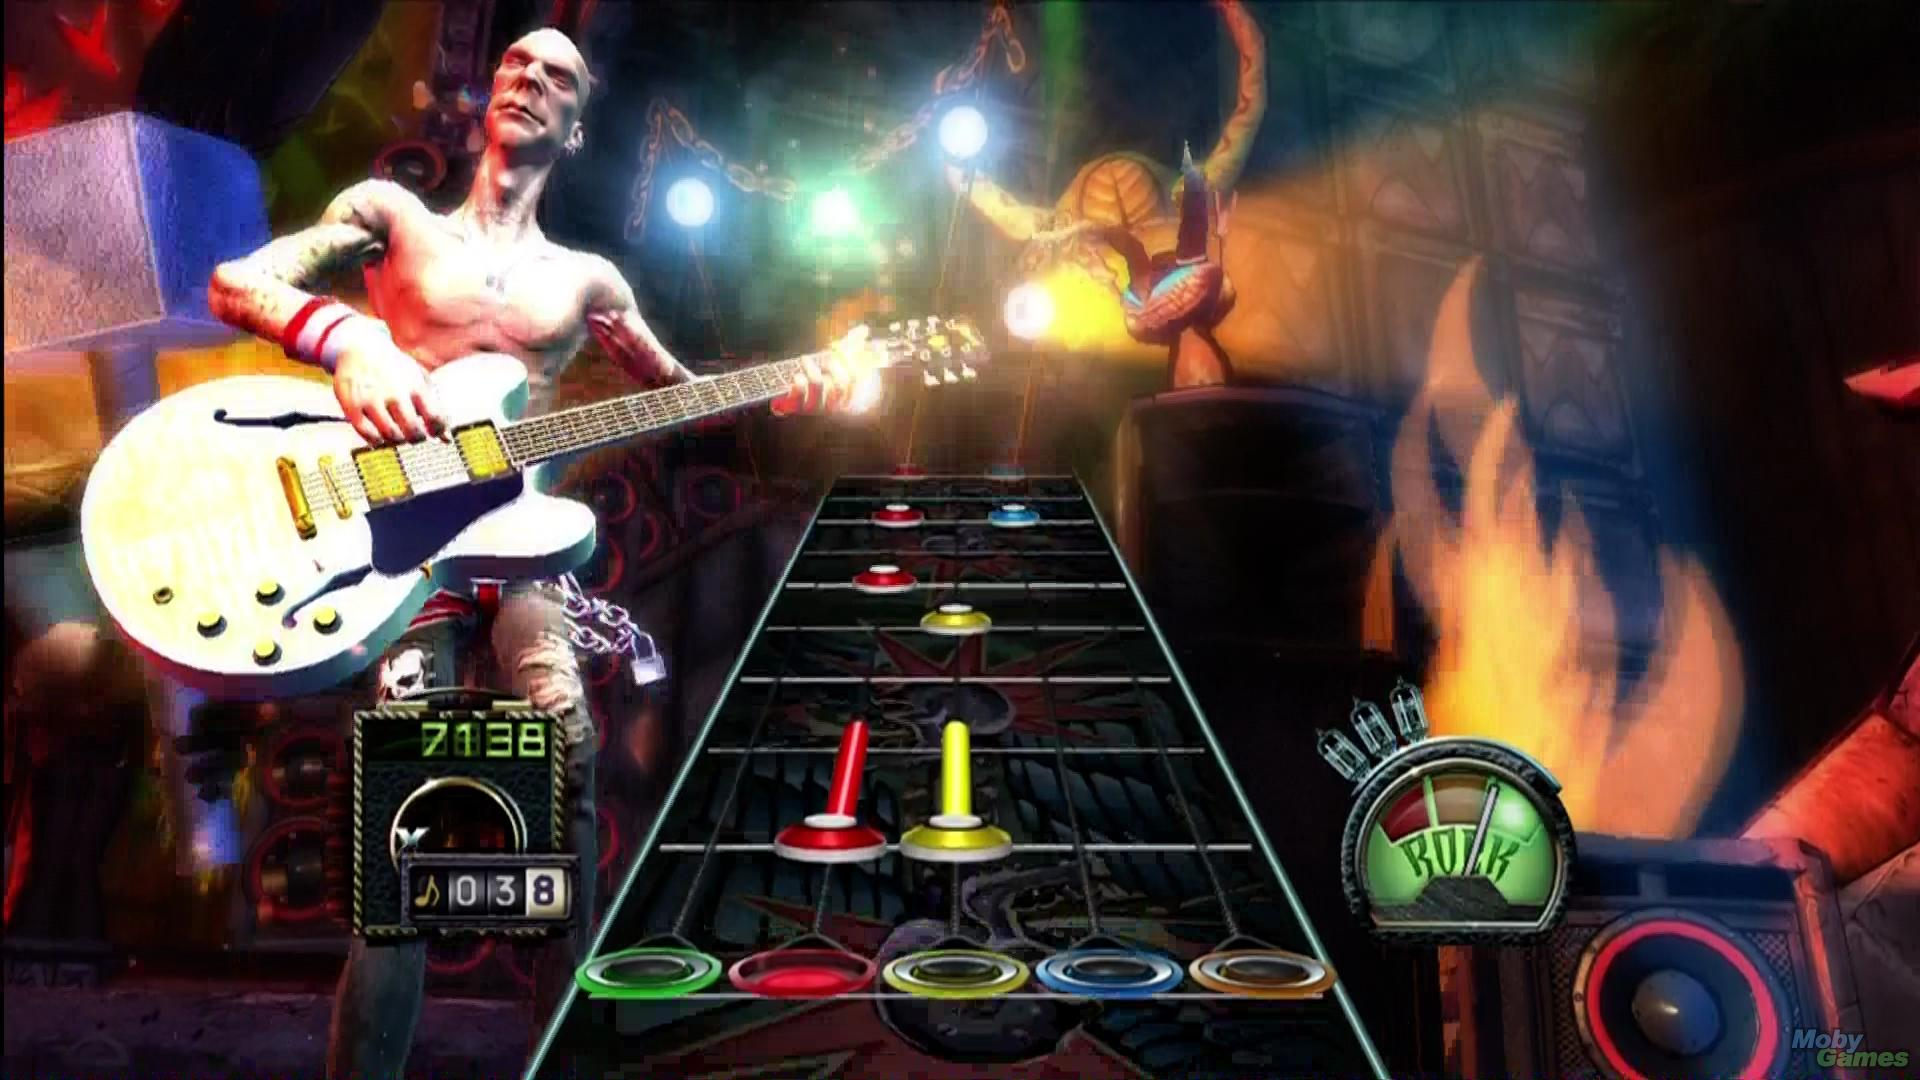
\includegraphics[width=0.7\linewidth]{figure/Analysis/guitarhero}
	\caption{Interactive music video game guitar hero.}
	\label{fig:guitarHero}
\end{figure}



\subsection{Noteput} 
Noteput is an interactive music table with tangible notes. It is made for learning notation. The idea is that you use the interactive screen that shows a staff which can be either a Treble Clef or Bass Clef, thereafter you can choose between the different notations and place them on the staff to determined if they should be whole, half, quarter, eights, sharp, flat or natural notes. The table also has an option to play the music or loop the music so the user can keep changing the sounds as the loop keeps playing.   
\begin{figure}[H]
	\centering
	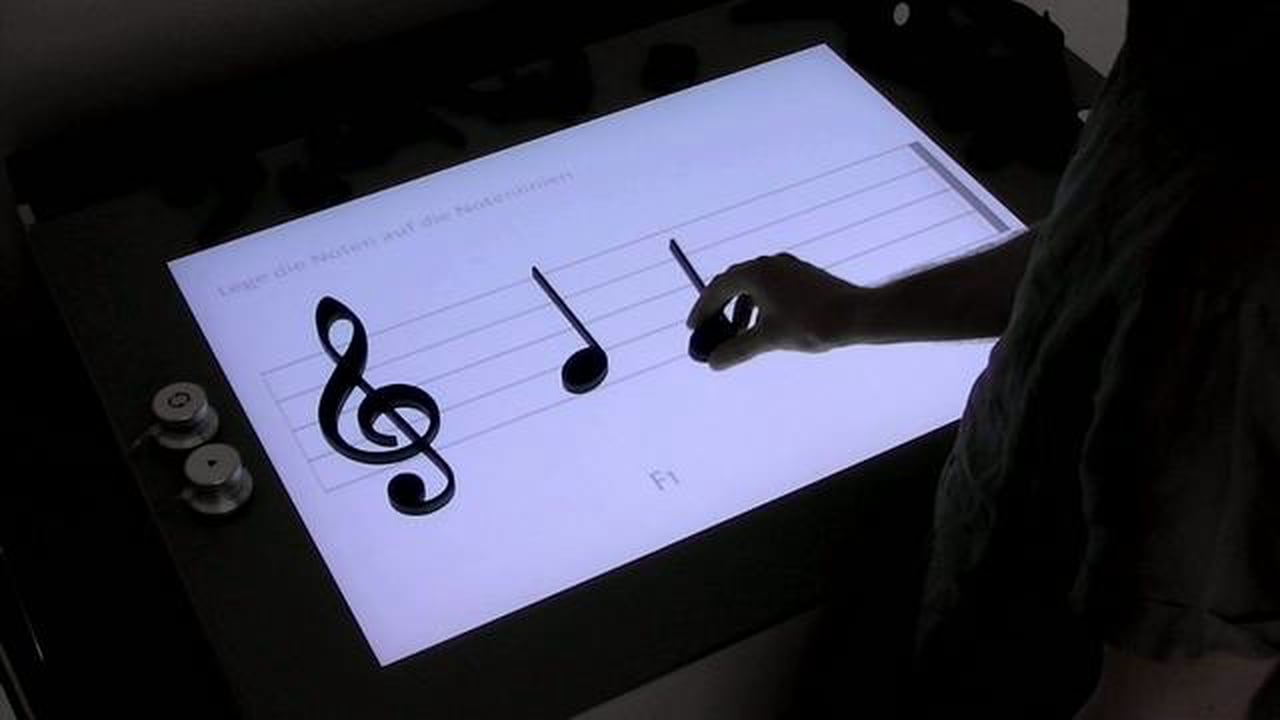
\includegraphics[width=0.7\linewidth]{figure/Analysis/noteput}
	\label{fig:noteput}
	\caption{Noteput}
\end{figure}


\subsection{Dato duo} 
Two person synthesizer for kids, no apparent learning outcome, but seems fun to play around with. Dato duo is a combination of a synthesizer and sequencer for creating electronic music together with people. It can be played alone or with others. It is meant to target children and adults interested in making music. On one side it is build using the circular sequencer which is a loop that loops the last eight notes that is played and playing a melody into it using the pentatonic keyboard (for example like using the black keys on a piano). On the other side are the controls for the synthesizer which contains two sliders that controls the two digital oscillators and the filter-cutoff frequency. It can also be combined with MIDI components and a sync input and output. 
\begin{figure}[H]
	\centering
	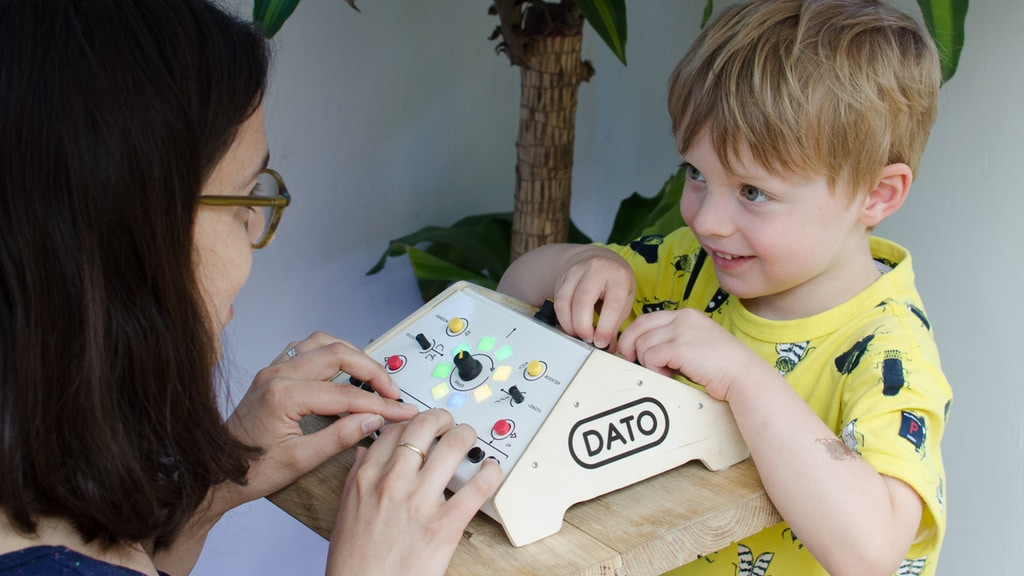
\includegraphics[width=0.7\linewidth]{figure/Analysis/datoduo}
	\label{fig:datoduo}
	\caption{Dato duo synthesizer}
\end{figure}

\subsection{Drop mix}
Dropmix is a hardware instrument for creating, freestyling, competitive or partying with music. It uses a large board with 5 different slots for placing cards of different values. It is operated by using a phone or tablet for playing each different mode which are clash, party and freestyle. Clash mode is a competitive game for 2 to 4 players. The goals of the game is to be the first team to reach 21 points. Each card that is placed on the table scores a point. To replace a card in one of the slots, it must be either equal or a higher level than the card already in the slot. Each card has to be placed into matching colored slots. There are also multicolored wildcards and black and white effect cards that can be placed onto any of the 5 slots. In party mode all players play together to play cards for mixing music and score points. The goal is to get the high score the crowds request as fast as you can. Request will then appear on the screen for a limited amount of time. Request can be for cards with certain level, color or instrument. Freestyle mode is all about mixing the different cards to create various beats. When you see the DM icon press the Dropmix button to spin the equalizer if the equalizer lands on the level then remove all the cards from that spot equal to the cards of that level. If it lands on the X clear all slots. The faster you meet each request the more points you will earn.

\begin{figure}[H]
	\centering
	
\includegraphics[width=0.7\linewidth]{figure/Analysis/dropmix}
	\label{fig:dropmix}
	\caption{Drop mix}
\end{figure}


\subsection{Dance Dance Revolution}
DDR is a physical interactive dance platform created by the Japanese company Konami. Players will stand on this platform and press the colored arrows on the stand of the platform corresponding to the arrows that will be shown on the screen. Each player will then be judged on how they time their dance patterns. There are a variety of music to choose from and when picking one the screen will show arrows that the user must imitate to receive points. 
\begin{figure}[H]
	\centering
	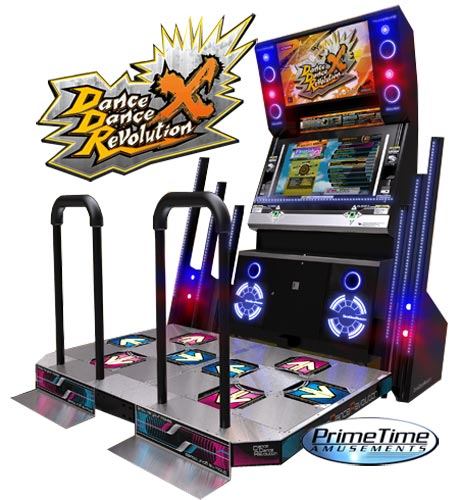
\includegraphics[width=0.7\linewidth]{figure/Analysis/dancedance}
	\label{fig:dancedance}
	\caption{Dance Dance Revolution}
\end{figure}

\subsection{Just dance}
Just dance is a dance video game developed by Ubisoft Milan and Ubisoft Paris. The game was released mainly for usage on Wii. The whole idea about the game is that each user must mimic the motions of an onscreen dancer’s choreography. For each movement the user will get more points. 
\begin{figure}[H]
	\centering
	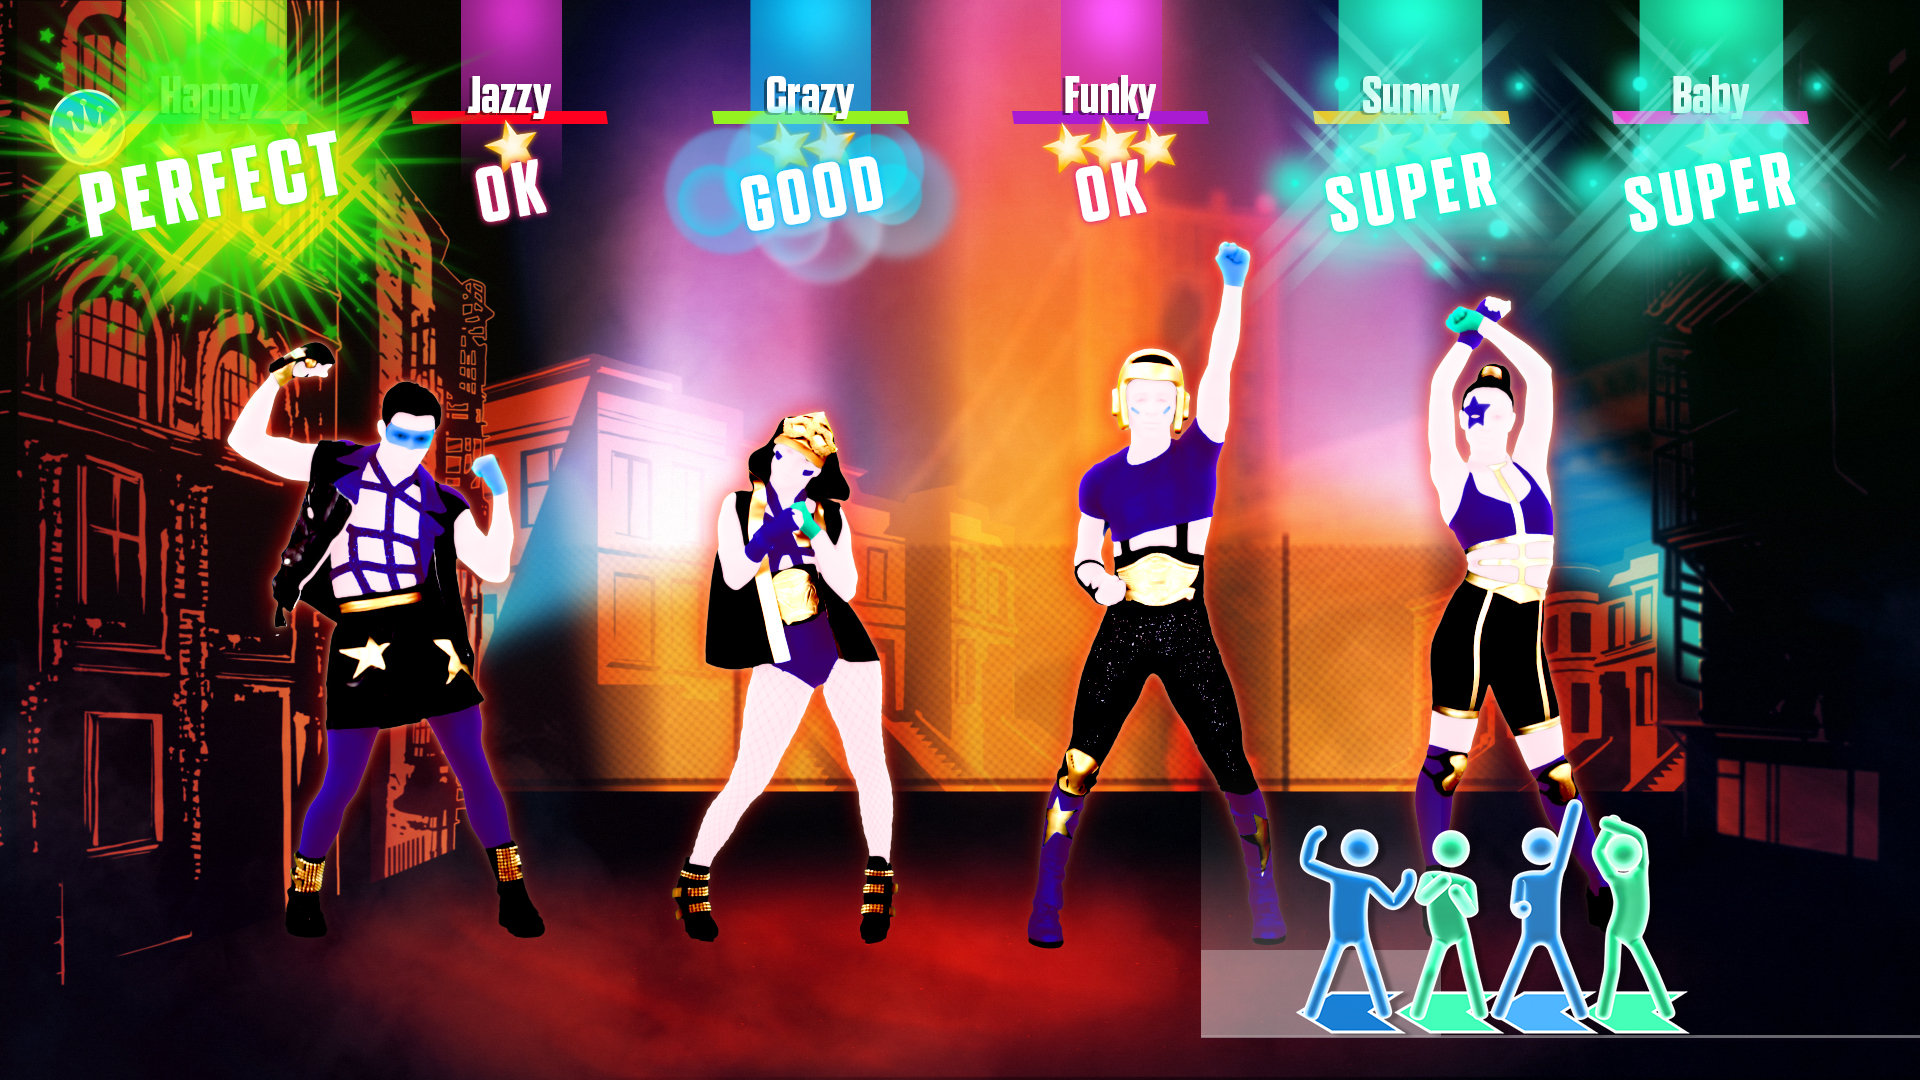
\includegraphics[width=0.7\linewidth]{figure/Analysis/justdance}
	\label{fig:Just Dance}
	\caption{Dance dance}
\end{figure}



	 
	\subsection{State of the art sub conclusion}


\section{Final Problem Statement}
	How can a physical interface facilitate collaboration for elementary school children aged 8-12 years in a musical education context?
	
\section{Design Requirements}
	\subsection*{Functional Requirements}
		\begin{itemize}
			\item[-] It must accommodate at least 2 children.\\
			\item[-] It must accommodate max 6 children.\\
			\item[-] Must facilitate collaboration within at least one of the three musical areas of competence.\\
			\item[-] Must be designed for Children aged 8-12.\\
			\item[-] It should strive to not induce  negative emotions.\\
			\item[-] It should strive to induce positive emotions.\\
			\item[-] It must be designed for use in a classroom setting.\\
			\item[-] It must output sound.
		\end{itemize}
	\subsection*{Non-Functional Requirements}
		
	
















		

% METHODS
\chapter{Methods}\label{chap:methods}
Based on the knowledge acquired in \autoref{chap:analysis}, the final problem statement and the design requirements, this chapter outlines the general strategy for answering the final problem statement.
\section{Design}
To come up with a design that can be implemented in a prototype that should be able to answer the final problem statement (see \autoref{sec:FPS}), multiple idea generation phases had to be conducted. As a part of these phases, an ideation workshop was run in collaboration with children from a Sankt Annæ 4th grade class (see \autoref{sec:methodWorkshop}).\\\\
We will create some design proposals based on the aforementioned feedback, and analyze them using a method akin to the Crawford slip method\cite{crawfordSlip}. To do this we will lay out the drawn ideas on a table, and every group member will write down what they think are positive and relevant elements of each idea on slips of paper. These slips will then be analyzed and be used to define the next iteration of our design.

\subsection{Usability}
The first usability test was conducted during the workshop with the children at Skt. Annæ school in the form of an early paper prototype. The feedback provided was brought back and used to create the next iteration of the prototype. \\
The next iteration was created without contact to the users due to not having the time and resources available. This iteration would be implemented and made ready for the initial usability test which will be conducted on Aalborg university Copenhagen.
The usability test will be in a controlled setting using the system usability scale (SUS) method, observation method and a think aloud test. The goal is to find out how the users perform on typical tasks, that are designed for them (the target group). 
The usability test will first conduct information from observation and a think aloud test. There will be 1-2 observers and the whole interaction should be exploratory for the tester. \par
Here are the bullet points for what will be observed during the usability test:\par

\begin{itemize} 
\item 	Observe how the person touch/interact with the pads. 
\item	Observe if they know or can figure out how to go from different octaves. 
	\begin{itemize} 
		\item 	Is it logical? 
		\item 	Do they maybe think the buttons are used for volume? 
	\end{itemize} 
\item 	Observe if the pads are too small or too big.
\item 	Observe how hard they must press on the pads. 
\item 	Observe if they understand the concept or what the interactive interface should be used as. 
\item 	Observe how they interact with the console/controller (the box)
\end{itemize}
\par
Here are the bullet points for what the users should be explained to do during the test: \par
\begin{itemize} 
\item 	Think aloud test:
	\begin{itemize}  
		\item 	Ask them to play 6 sounds 
		\item 	Ask them to go down an octave and play 6 sounds
		\item   Ask them to go up an octave and play 6 sounds
		\item 	Ask them to record a sequence
		\item   Ask them to play the sequence they recorded
		\item 	Ask them to explain the different components 
	\end{itemize} 
\end{itemize} \par
It will be conducted by recording the behaviours of the target group and below are the ten sample questions from the SUS method. The ten sample questions will be shown at the end of the usability test. Each user has to answer the below questions. \todo{This doesn't belong here, move to design.}
\par
\begin{enumerate} 
\item 	I think that I would like to use this system frequently.
\item 	I found the system unnecessarily complex.
\item 	I thought the system was easy to use.
\item 	I think that I would need the support of a technical person to be able to use this system.
\item 	I found the various functions in this system were well integrated.
\item 	I thought there was too much inconsistency in this system.
\item   I would imagine that most people would learn to use this system very quickly.
\item 	I found the system very cumbersome to use.
\item 	I felt very confident using the system.
\item 	I needed to learn a lot of things before I could get going with this system.
\end{enumerate} 
\todo{Move this to appendices}
\par
 
  Depending on the results of the usability test or using convenience sampling around the campus on Aalborg University Copenhagen(AAU CPH), another iteration will potentially be created and then usability tested again. Both tests will be conducted using the System Usability Scale (SUS)\cite{susScale}. Item 8 in the SUS scale will be reworded so the word \textit{"cumbersome"} will be replaced by the word \textit{"awkward"} to eliminate confusion\cite{susScale}.\todo{Dette afsnit skal laves om da vi ikke kunne teste usability til midterm}
	
\section{Evaluation}
Quantitative test and then qualitative test.
Explanatory sequential mixed methods\cite[p.~21]{bjoernerBog}

Do Pilot test on both tests, using convenience sampling.

Testing with children\cite[p.~207]{bjoernerBog}.

Likert scales

Cronbach alpha checks correlation between two variables
Ideal correlation:

0.9 Excellent (Never seen in practice)

0.8 Great

0.7 Acceptable

<0.5 WRONG

Make test that answers problem statement.

Think about them variables yo.

Sankt Annæ not necessarily representative of target group.

Population sample might be more interested in music and have prior musical knowledge.

\subsection{Crunch data}
	We will do some math here.\cite{nyBog}

% DESIGN
\chapter{Design}

In this chapter, the process of deciding upon and making the design of the Physical interface (music educational tool), will be explained. The design will be based on the formulated design requirements (see \autoref{sec:DRequirements}), as well as the common design principles of Gestalt \cite{gestalt}, the SOTA ( \autoref{sec:sota}) and knowledge gained from the workshop at Sankt Annæ (see \autoref{sec:workshop}). 


\section{Intial design}
The design of the physical interface was, with the design requirements, not specified to the extend, that a specific concept for the design was obvious. The design could instead be taken in broad variety of directions, and still live up to the requirements. As so, the design of the physical interface has been though lots of different concepts and iterations. 

\subsection {Workshop prototypes - The pre-initial designs}

During the analysis, a need for educational tools that were built with collaboration in mind, was discovered (see \autoref{sec:problemArea}). Based on that, multiple low fidelity initial concepts were created and brought to Sankt Annæ for an ideation workshop. As mentioned in \autoref{sec:problemArea}, the prototypes at this point were used to discuss and discover new concepts and elements, which could be utilized in the final design. The findings from this workshop did not necessarily lead to new requirements, but instead served as pointers to which direction the design could be taken. For example, the tool could make use of movement, which might conflict with or move the focus away from the learning aspect, and (in such a case) should be avoided. In another case, movement might serve to enhance the learning outcome (see \autoref{AnalysisMovement}), and should therefore be strived for. This however depends on the individual concept, and each find from the workshop should therefore be discussed in relation to each design idea.\\\\

In order to evaluate upon many different elements and ways of collaborating and learning music, the aim of the concepts behind the prototypes, was to differ significantly from one another. Both the topic of the material to be learned, and the way to work with this, was therefore different for each of the concepts. Each concept will be briefly described in the following figure \todo{make figure}.
\todo{lav "collage" med ideer og giv kort beskrivelse af concept ( ryste klods,joystic band,chord master felx ,frugt løkker,quizz game, sequencer square..   A physical version of \textit{Garage Band}. }

\begin{figure}[H]
	\centering
	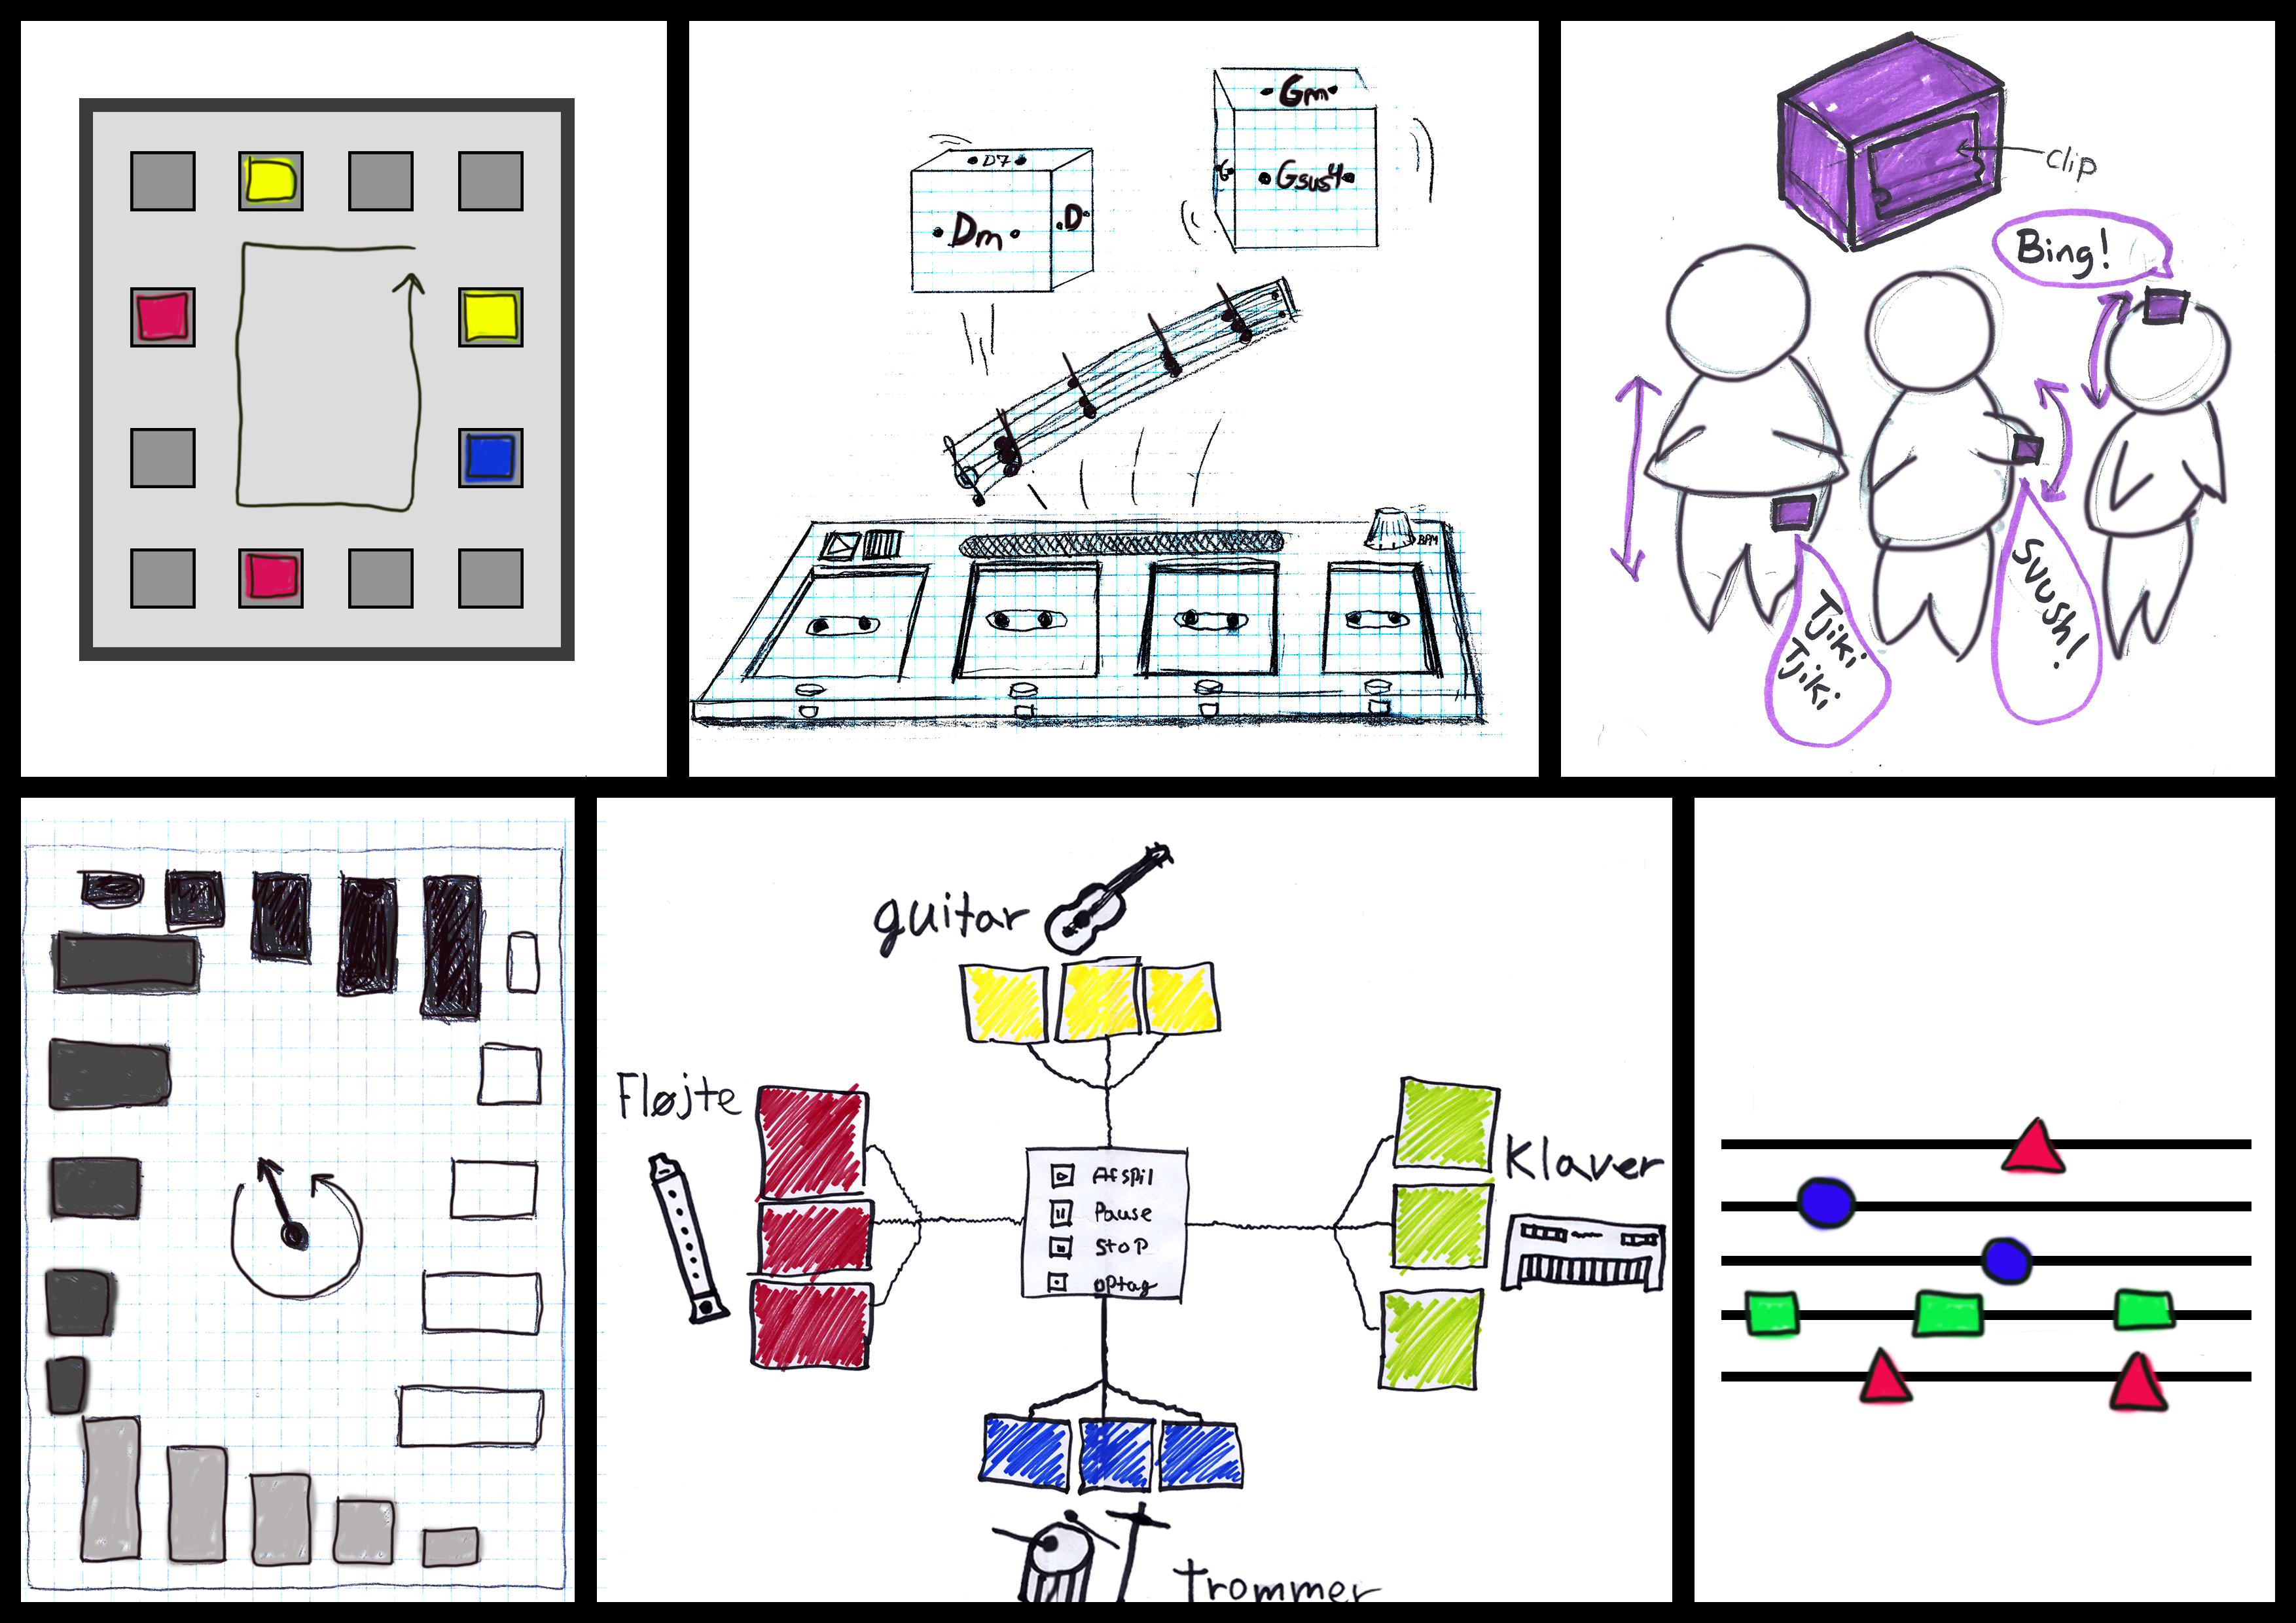
\includegraphics[width=0.9\linewidth]{figure/Design/workshopPrototypesDone} 
	\caption{Seen is the 6 design concepts which were precented at the workshop at Sankt Annæ. Top left: a device that loops though entries(squares), and plays sounds if a box is placed on the entry point. Top middle: an ear training tool, where boxes labeled with tone names, should be orientated to display the heard tone. Top right: Wearables which produces individual sounds when shaken. can be used to create and perform music - alike STOMP. Bottom left: Board of a quiz game with music theory questions. Bottom middle: A set of joysticks to play instruments in a "band setting". Bottom right: A physical version of \textit{Garage Band}\cite{Garageband}.}
	\label{fig:workshopPrototypes}
\end{figure}
\todo{erstat med "collage" med ideer og giv kort beskrivelse af concept ( ryste klods,joystic band,chord master felx ,frugt løkker,quizz game, sequencer square..1. quiz game with music theory questions  2. Wearables which produces individual sounds when shaken. can be used to create and perform music - alike STOMP 3. a set of joysticks to play instruments in a "band setting". 4. A physical version of \textit{Garage Band}. 5. loops though entries, and plays sounds if a box is placed on the entry point. 6. Ear training tool, where boxes labeled with tone names, should be orientated to display the heard tone.}



\subsection{From workshop and requirements - the Crawford slip method}
To evaluate upon the workshop prototype concepts, in relation to the design requirements formulated and the knowledge gained from the workshop, a custom version of the Crawford slip method was used (\autoref{secc:designMethod}) \todo{fix label then method is done!}. By doing this, a list of suggestions to how elements could be used, and should not be used, was made and used as inspiration for other concept ideas. A sample of the list can be seen in figure \autoref{fig:snippetOfList}. The full list can be seen in the appendix \autoref{CrawfordSlipList}.  

\begin{figure}[H]
	\centering
	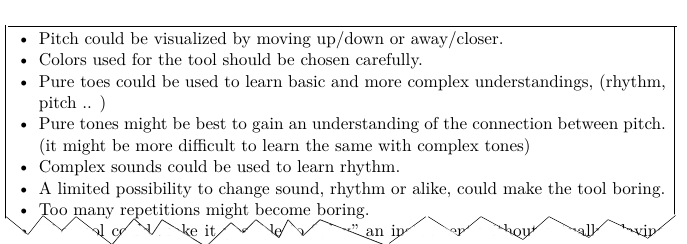
\includegraphics[width=0.7\linewidth]{figure/Design/snippetOfList} 
	\caption{Seen is a small section of the design suggestion list, based on the custom version of the Crawford slip method.}
	\label{fig:snippetOfList}
\end{figure}


With the project group divided into two groups of three persons, two design concept was created (one for each group), with inspiration form this list. These two concepts, was then presented between the two groups, and discussed.  

\subsubsection{Concept proposal 1: a variation af the \textit{"Simon Says"} game }
This design concept was highly inspired by the electronic game of \textit{Simon says} \cite{simonSays} - a musical memory game, where the player must repeat a sequence of tones generated by the game, by pressing the corresponding buttons on the interface. The idea was, that each student would have their own four push buttons, corresponding to the ones from the original game - see \autoref{fig:SimonSaysAlike}. The first player would then start the game, by choosing the first tone for the sequence, by selecting one of their buttons. the next player should then repeat the tone by pressing their equivalent button, and then add to the sequence by selecting the next tone. The players will continue taking turns until a player fail to repeat the sequence. This player will then no longer be part of the game, and must wait until the rest of the players have either failed to repeat the sequence, or won the game by being the last player left.

\begin{figure}[H]
	\centering
	\includegraphics[width=0.7\linewidth]{figure/Design/SimonSaysAlike} 
	\caption{Seen is the concept idea of a memory game alike \textit{Simon Says}. Each edge of the figure contains a set of four buttons, which belongs to a player. The players must take turns in memorizing, repeating, and then adding a new tone to the sequence, by pressing the buttons. Turn taking is visualized with LEDs}
	\label{fig:SimonSaysAlike}
\end{figure}

This concept relates to the study plans section of \textit{Musical creation }(\autoref{sec:studyPlan}), by having the element of improvisation when having to pick the next tone. The concept may be used to play melodies together, or (as intended) as a competitive game. Either way, the students could learn (through ear training) to understand the tonal context between the four tones used in the game.   

\subsubsection{Concept proposal 2: Sequencer Mat}\label{sequencerMat}
This design concept evolved around the idea of a mat, which should function as a sequencer (a tool to play and record sequences of sounds). The Mat should allow the user to actively perform sounds in form of pure tones, by stepping on fields indicated as a grid on the mat. A sketch of the interface for this concept, can be seen in \autoref{fig:firstSketchOfMatFig}. Each field on the vertical axis, should produce a single pure tone which should be different from the others. These tones should relate to a scale ( e.g:  C,D,E,F,G,A,H). Each field along the horizontal axis, should produce the same pure tone. The sequencer functions -which could be: play, record, save, add new, reset, different channels, and adjust pace - should be controlled by buttons placed along the side of the mat, or near same.     

\begin{figure}[H]
	\centering
	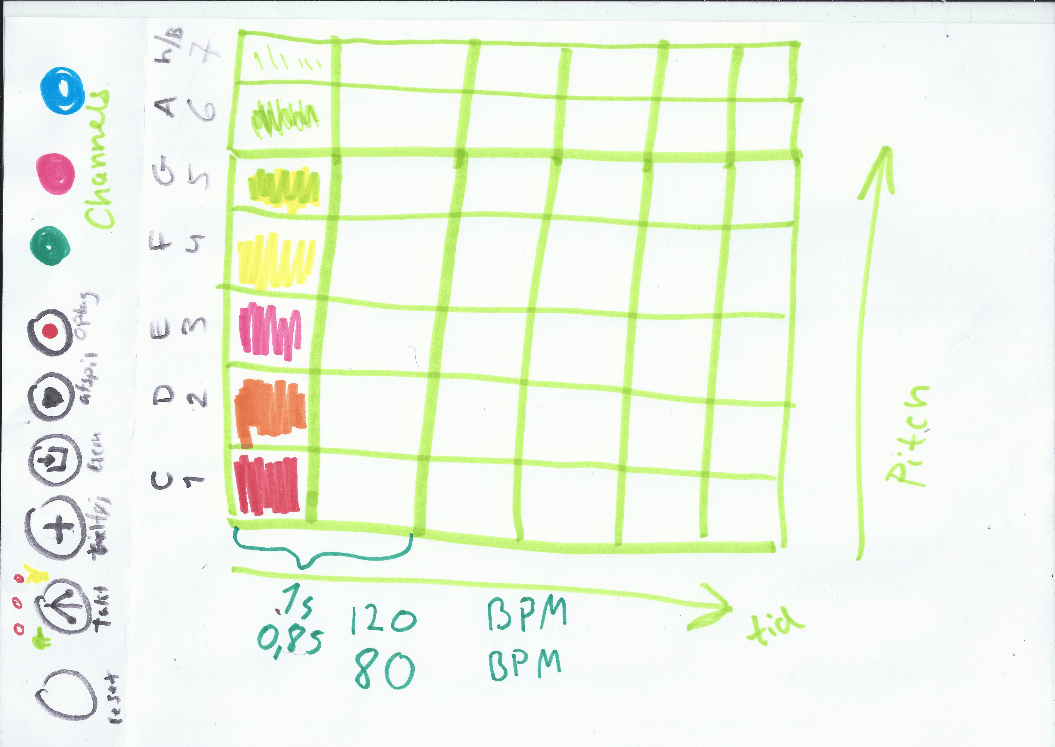
\includegraphics[width=0.9\linewidth]{figure/Design/firstSketchOfMat} 
	\caption{Seen is the first sketch of the interface for the sequencer-Mat concept . In the middle of the figure, is a green 7x6 grid - each field should activate a sound when stepped on. The horizontal axis of this grid, indicates time. The vertical axis indicates pitch of the sound. The pitch is also indicated by a color scheme along the same axis, variating from a dark to a light color. This is illustrated in the first column of the grid. Along same axis are the tone names stated besides their given rows. To the left of the grid are 9 push buttons (drawn as circles) with different functions (indicated with symbols and text) placed vertical. }
	\label{fig:firstSketchOfMatFig}
\end{figure}

To clarify how the basic sequencer functionality (play and record) should function, an example of a use case has been made. \\
\paragraph{Example of an use case}
Three students wants to play and record a set of tones which they want to consists of 3 tones with a break between each tone. They wants to play the tones F, C and G, respectively. The students place themselves on the mat, which the most left field activated (stepped on) being the tone F, then an empty column, then an activated field of the tone C, one more empty column, and lastly an activated field of the tone G. As so, it can be seen, that the tones are played from left to right.   
\begin{figure}[H]
	\centering
	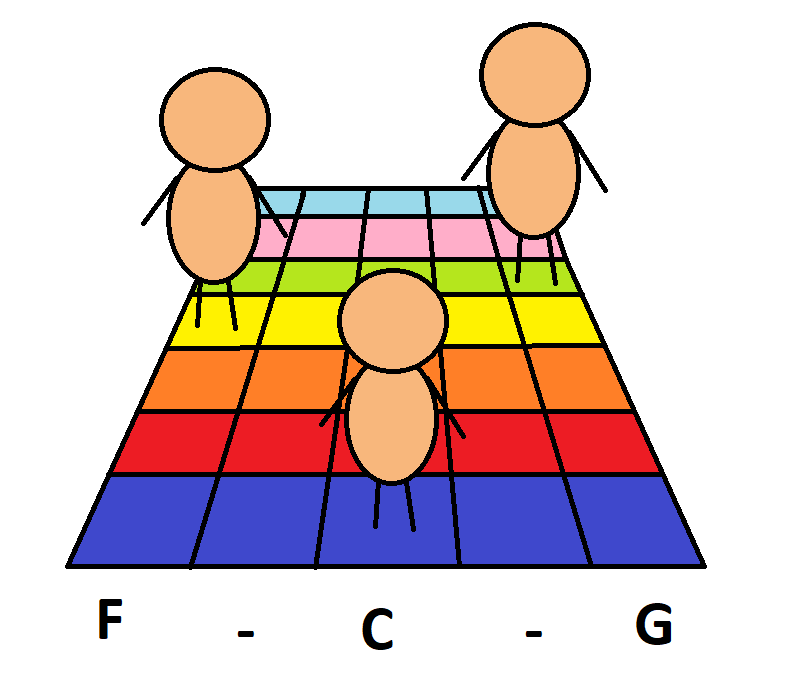
\includegraphics[width=0.7\linewidth]{figure/Design/UseCase} 
	\caption{Seen is an example of a use case of the sequencer mat tool. Three students are using the tool, recording the tones in the order of F, break, C, break, G. }
	\label{fig:UseCase2}
\end{figure}
  

To conclude on the two proposals, this (sequencer mat) concept included more of the desired elements gained from the workshop (\autoref{sec:workshop}), as well as having a more clear relation to the study plan (see \autoref{sec:studyPlan}) than the previous proposal,
it was therefore decided to continue working with this concept proposal (\autoref{sequencerMat}), as being the definitive design concept. 

\section{The Final design}\label{designConcept}
The concept, as explained in \autoref{sequencerMat}, was kept in the final design, however a lot of specification of functionalities and design was needed. These include the size, tempo, and musical scale of the mat, how the scale and time axis should be visualized, which functionalities (in form of buttons) should be implemented, where they should be placed, and how they should be visualized. 


\subsection{The setup}
The concept of the design includes visible functionality controls (buttons), and - without going far into implementation aspects of the design (is to be explained in \autoref{imp}), it was known that both these, and the mat itself, needed to be controlled by some electronics. For the sake of securing and protecting the electronic components, a box was chosen to become the housing of same, and as well, function as a interface for which the controls (buttons) should be placed. 

The placement of this control box in relation to the mat, was discussed, and it became clear, that the portability (so it could be transported for later testing), would have a high influence on the design. As it can be seen in \autoref{fig:matVsBox}, many different solutions were discussed. A suggestion was to have the box fasten along one side of the mat. Another was to have it fasten in continuation of the middle column of the mat grid, and maybe have the mat constructed to be collapsible. Lastly a suggestion was to make the mat and the box to be transported separately, and to be connected though a cable connector.     

\begin{figure}[H]
	\centering
	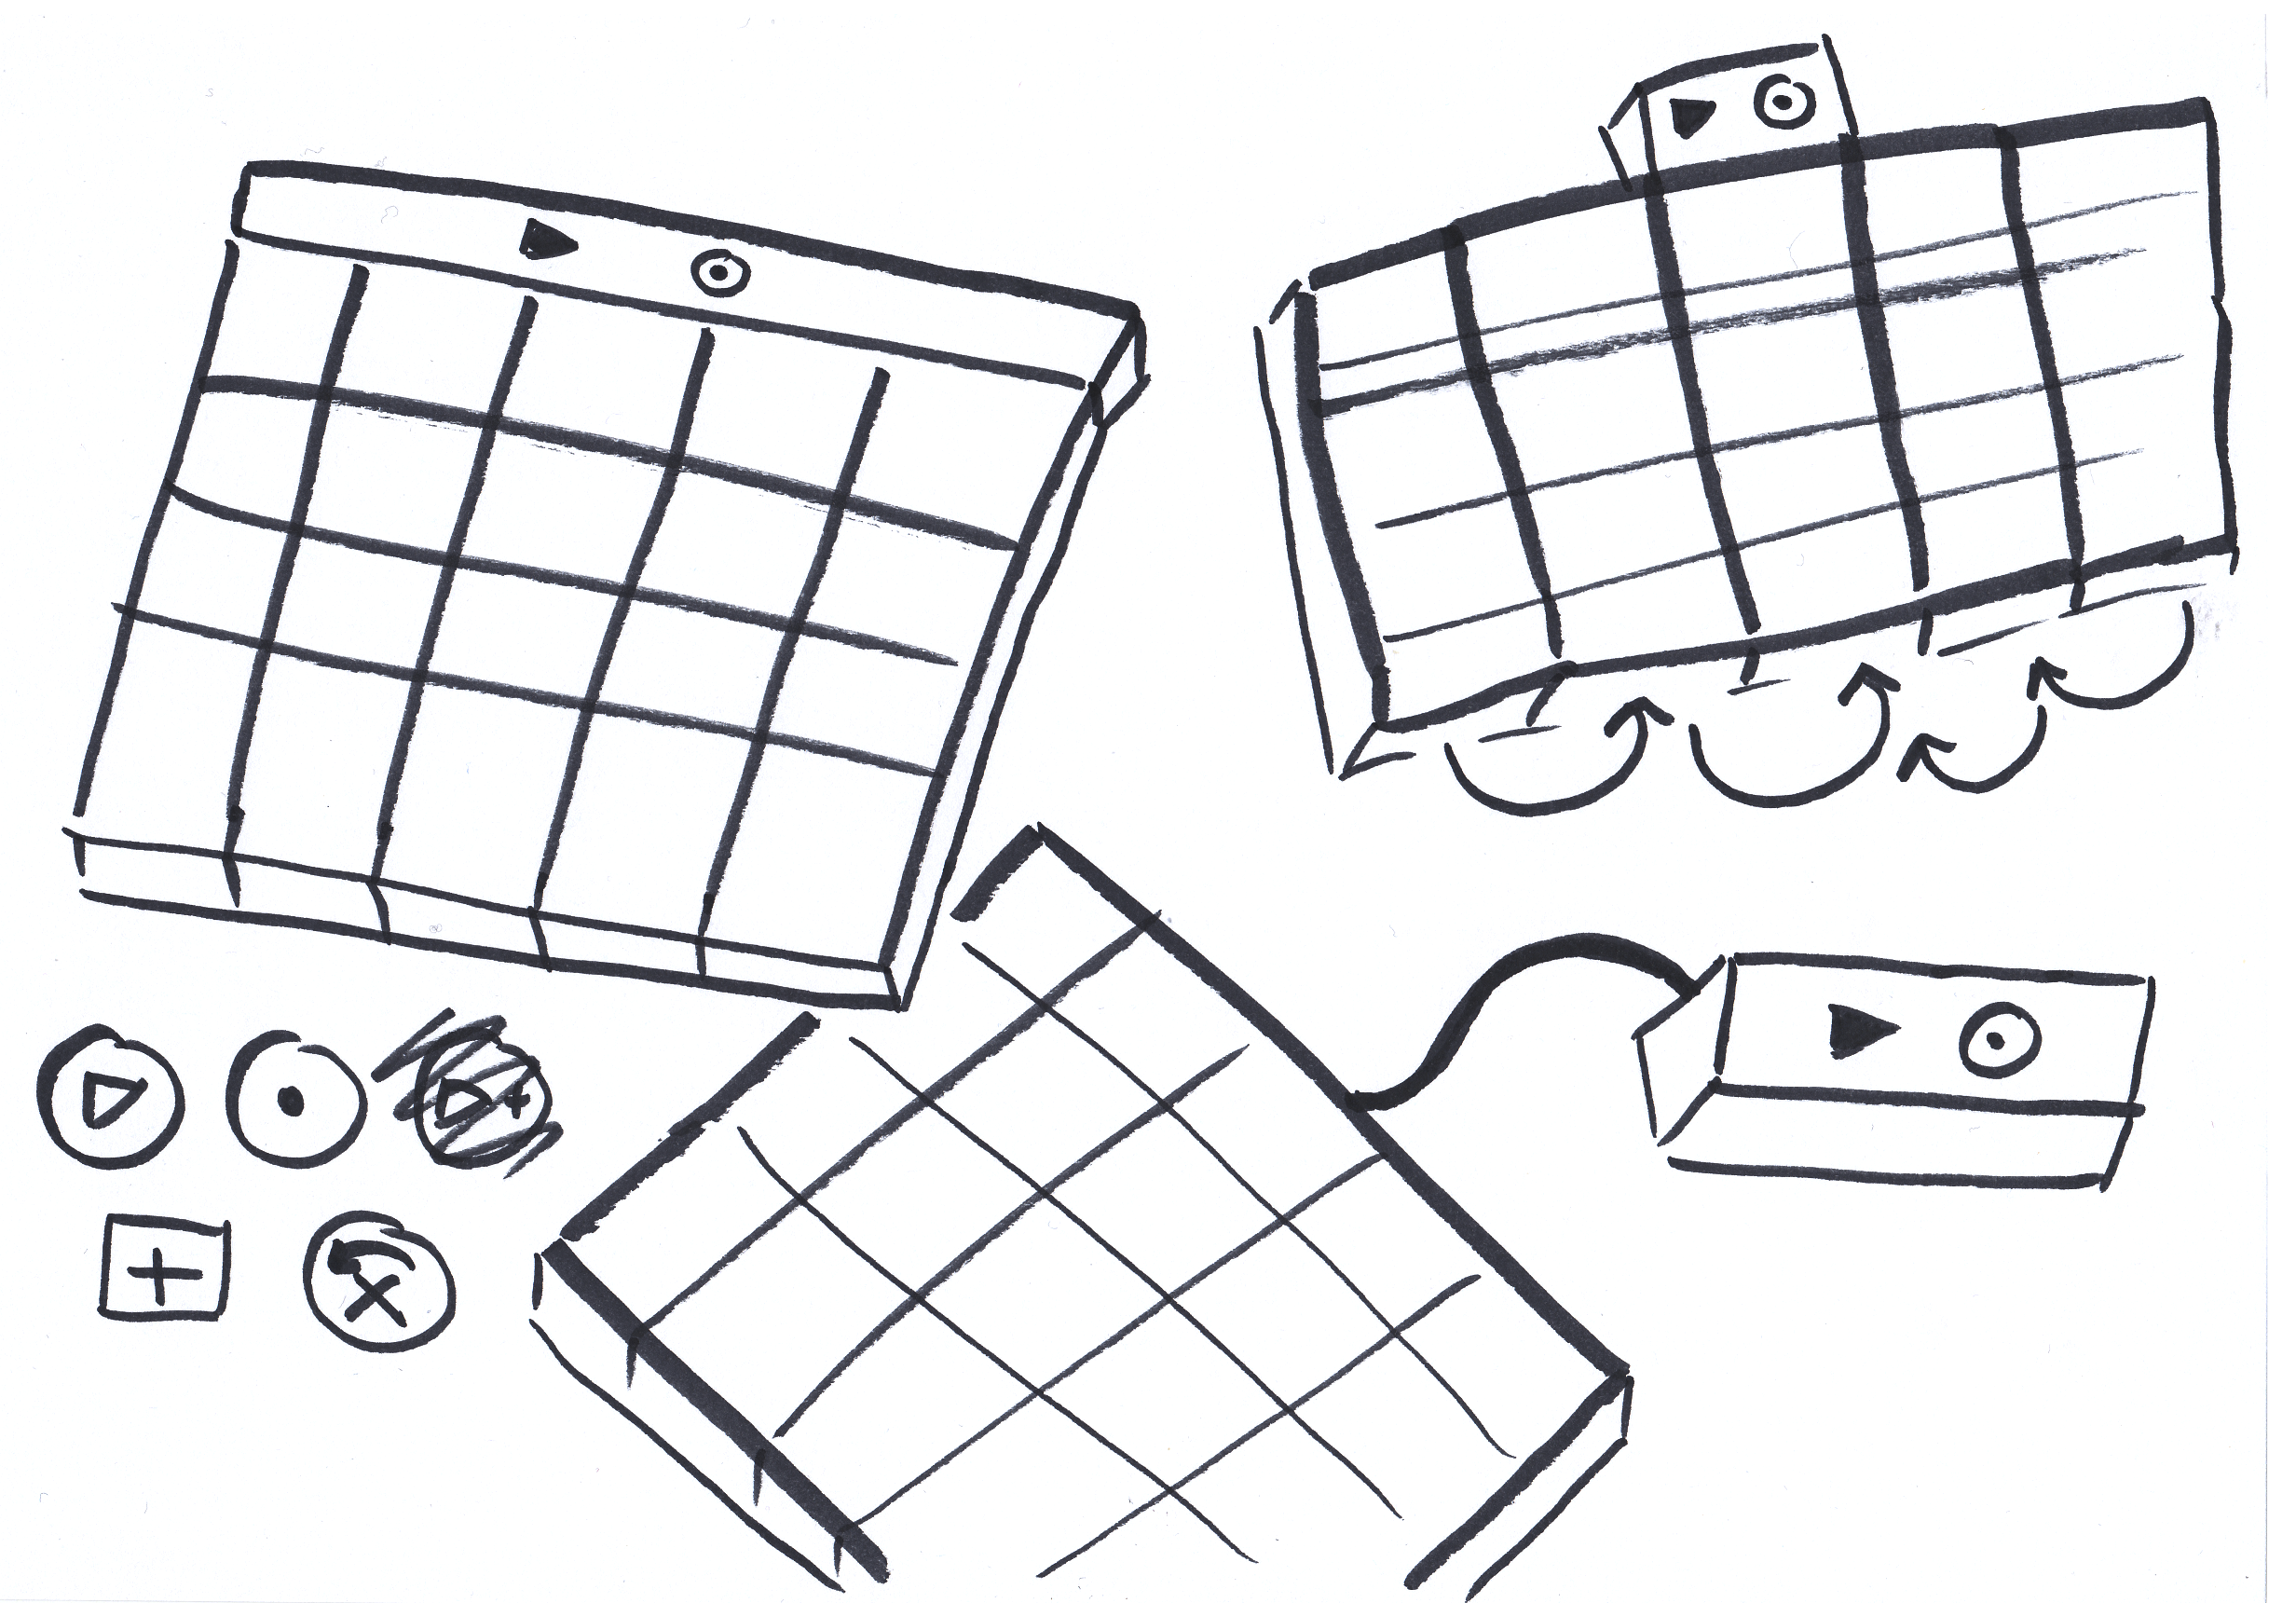
\includegraphics[width=0.7\linewidth]{figure/Design/maatteSetup}
	\caption{Seen is the different proposals to how the mat and box should be connected. Top left is the box fasten along the edge of the mat. Top right is the box fasten to the top of one column of the mat, which is collapsible. At the bottom is the box and mat connected though a detachable cable}
	\label{fig:matVsBox}
\end{figure} 

The material for construction the mat, was not yet chosen (Materials will be discussed in \autoref{theMat}), which made it uncertain if fasten the box(which was to be made of a hard material for protection of the electrical components), would be possible. For example if the mat was to be constructed by a flexible material, the connection joints between the mat and the box, might become overly exposed.
As the later of the suggestions, where the mat and box was to be manually connected though a cable, did not depend on the choice of material, this design was chosen. 


\subsection{The size and sound of the mat } \label{sizeSoundColorMat}
The size of the mat, effects the number of different tones it can produce, as the number of fields on the vertical axis is equivalent to the number of tones available. As this tool, should be used to create and perform music in an educational context (which relates to the study plan, see \autoref{studyPlan}), using a musical scale would be appropriate in relation to learning scales, and it would furthermore establish a hierarchy of the tones, due to the tonal context(which relates to the design principles\autoref{gestalt} of proximity and continuation) present in a scale \autoref{cognitiveFoundationOfPitch}, and thereby aid the student in understanding which field to stand on, to get the desired tone - making the tool more usable.  \\
Of the most common and primitive scales, are the major and minor scales (also called \textit{natural scales}), which consist of 7 notes (C D E F G A H/B - This is the C major scale) \cite{scales}. As one of these scales could have been chosen for this project, the \textit{Pentatonic scale}, which origins from the natural scales, have a few advantages for which it instead was chosen. The Pentatonic scale consist of five - hereof \textit{"penta"} - of the notes from the natural scale (C D E G A - this is the C major pentatonic scale), and has both the advantage of being able to be used in the same context as the natural scales, as well as sounding great no matter the combination of the notes \cite{pentatonicScale}. This makes this scale highly suitable for improvisational music, and beginners \cite{pentatonicScale}.  \\\\ 

With the pentatonic scale chosen for the tool, the vertical size of the mat was settled - 5 fields pr row. As the number of columns equivalents to the tempo of the sequencer function, and should therefore also reflect the musical aspect of tempo. A large variety of tempo could have been chosen, but as the most commonly used time is $\dfrac{4}{4} $ \cite{tempo}, this was decided as the rhythm of the tool. \\ As so, the size of the mat was decided to be 5x4 as seen on \autoref{fig:matSize}. As for the size of each field within the grid, the size of 27x27cm was chosen, based on the assumption that 4th graders have a shoesize ranging from size 35(EU) - 38(EU), which is approximately 22 - 25cm. This means that there will be room for one student pr field.       


\begin{figure}[H]
	\centering
	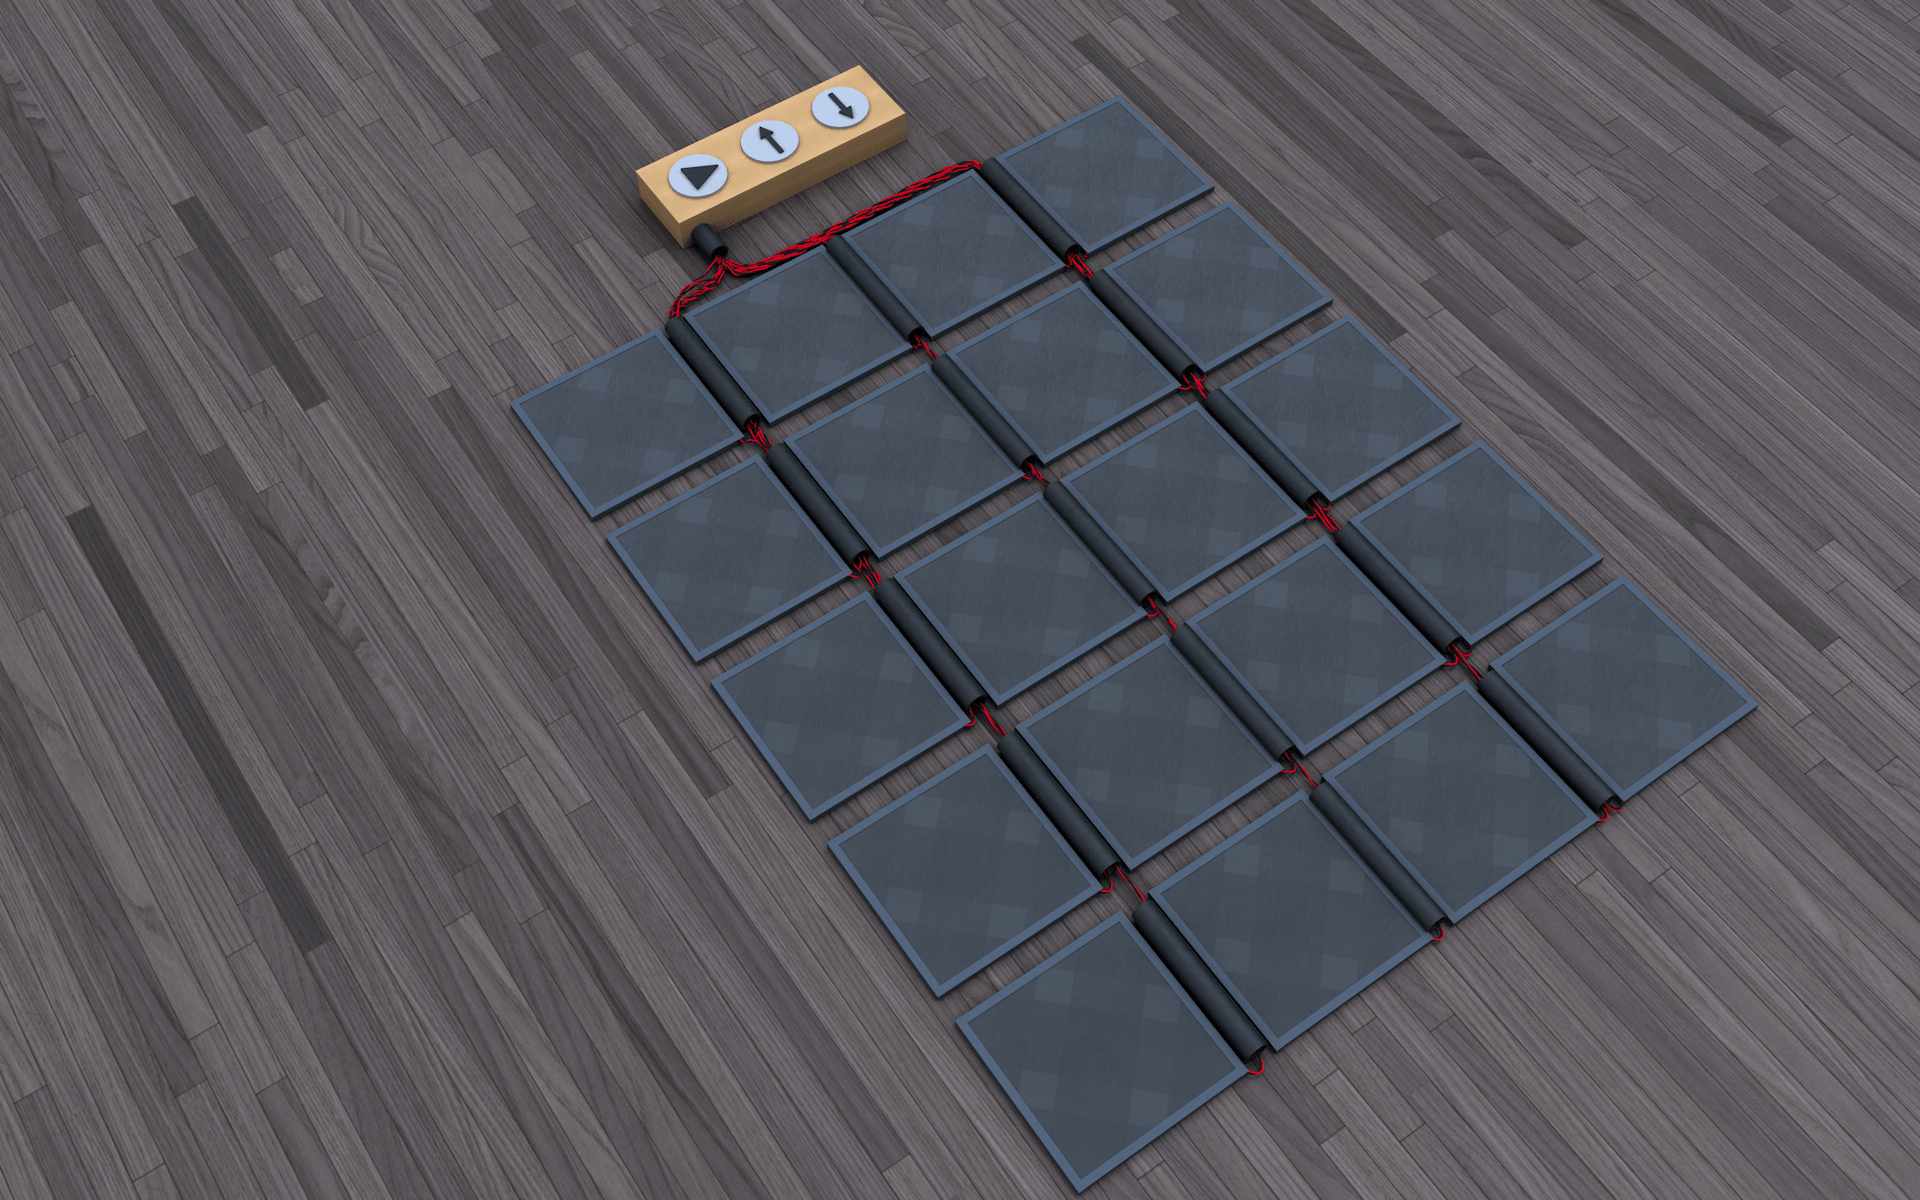
\includegraphics[width=0.8\linewidth]{figure/Design/finaldesign}
	\label{fig:matSize}
	\caption{Seen is a computer generated visualization of the size of the mat (a 5x4 grid), and the placement of the control box in relation to this.}
\end{figure}

To visualize the tonal context - ranging from a dark to a light tone, from bottom to top of the column - it was decided to use color to represent this transition. A color scheme was therefore to be chosen. Four out of five of the discussed color schemes can be seen on \autoref{colors} - missing is a gray scale gradient. The different color schemes discussed, was created with the intention of making a transition from a light to a dark color, resembling the tonal context. During the discussion, it became clear that the brightness of colors, was perceived different between individuals. For example could the green color be perceived brighter than the yellow by one person, while the opposite applied to another. To avoid confusion and ensure a common understanding for the transition, it was decided to use five different nuances/brightnesses of the same color. Two examples of this can be seen on \autoref{fig:colors}  - the two bottom ones. The orange color scheme was chosen, as this - in comparison to the blue, is often refereed to as a energetic color \cite{orange}, and was in relation to the physical active context of the tool, more suitable in the minds of the project group.               

\begin{figure}[H]
	\centering
	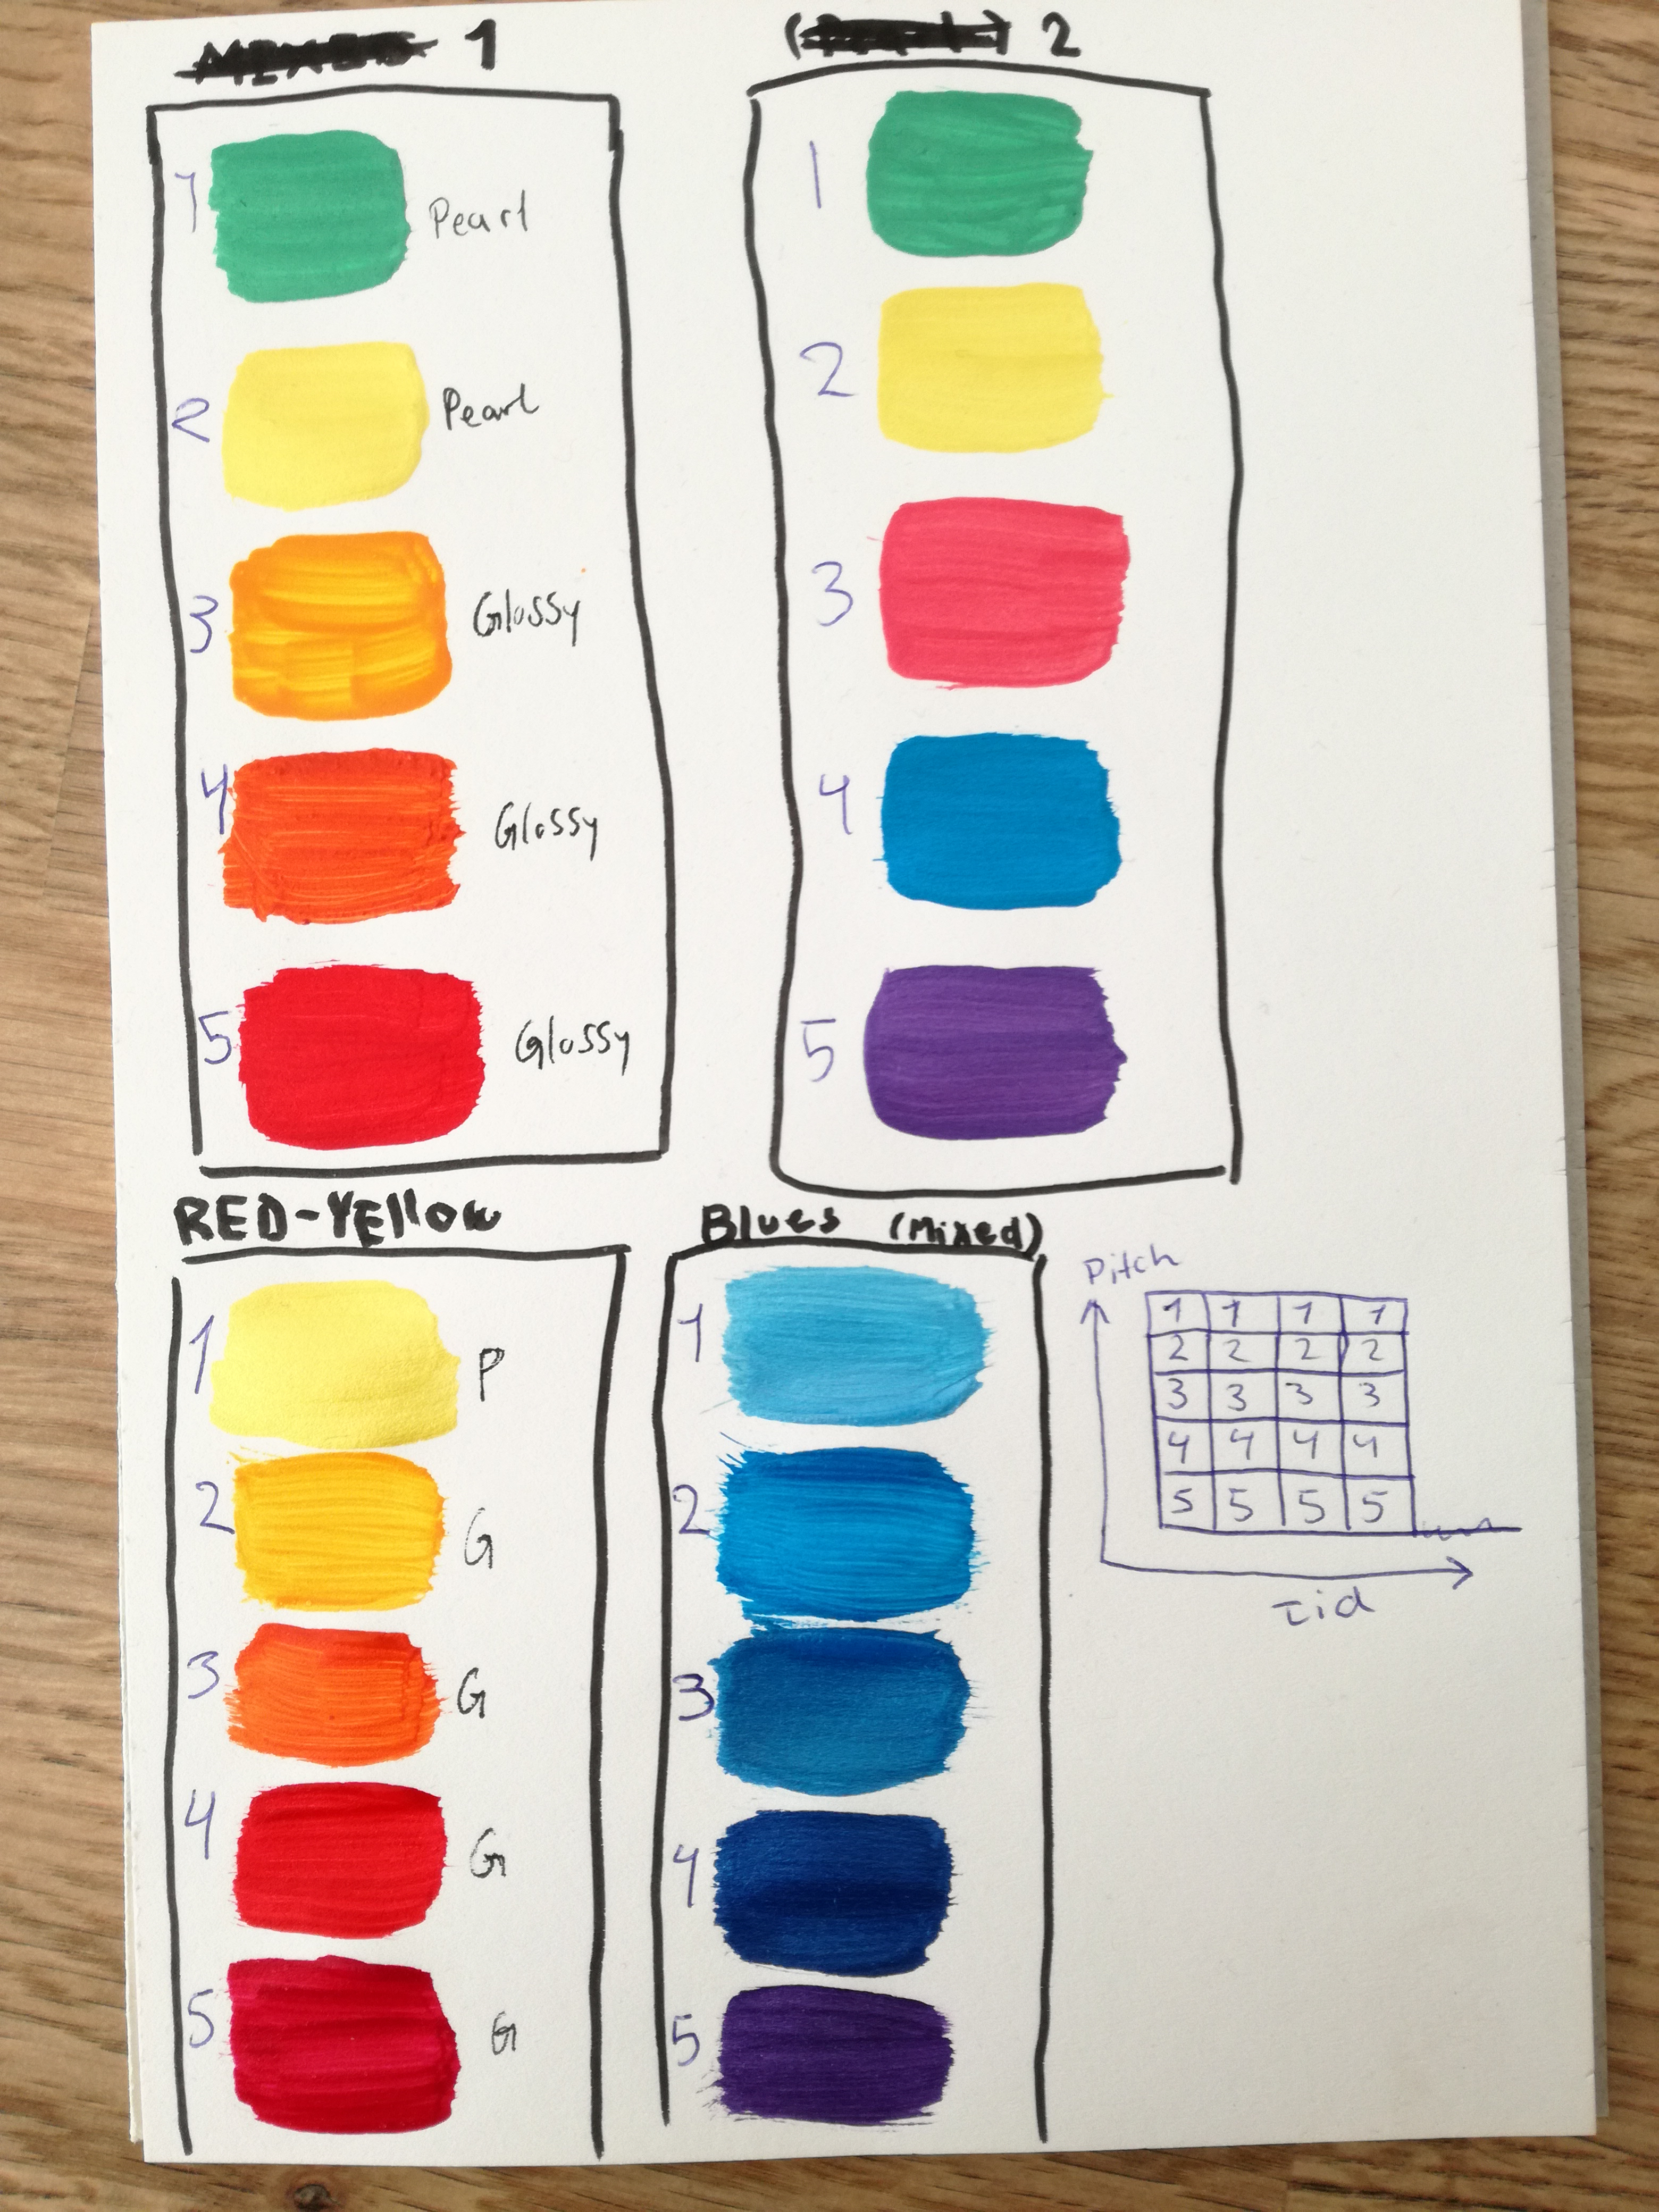
\includegraphics[width=0.5\linewidth]{figure/Design/colors}
	\caption{The four different color schemes (excluding a gray scale gradient), which was discussed for visualizing the tonal context.}	
	\label{fig:colors}
\end{figure}

To enhance the understanding of the columns as having the same tones, the design principle of similarity was used, by using the same color scheme for each column, as seen on \autoref{coloredMat}. \\
As so, by adding these decisions for colors and design principle, it should be visualized, that the fields with the same color, produce the same tone, and that each column contains one of each tone.  

\begin{figure}[H]
	\centering
	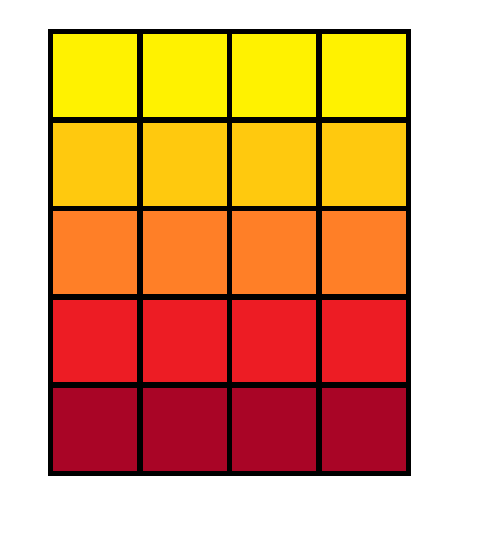
\includegraphics[width=0.5\linewidth]{figure/Design/coloredMat}
	\caption{Seen is a visualization of how the mat should be colored.}	
	\label{fig:coloredMat}
 \end{figure}


\subsection{The control box}
The control box functions, is as stated, both as protection for the hardware, as well as a interface for the controls of the sequencer. In this section, the thoughts concerning the dimensions of the box will be stated, and the functionalities for the sequencer and the visualizing of relating buttons, will be discussed.

\subsubsection{The dimensions} 
First of all, should the box be big enough to store the wires and components of the system. Besides this, the dimensions should take the use and possible misuse into consideration. With this is meant that actions such as using the controls on the box, should not make it fall over - it should be steady, and that jumping on the box (misuse) might be avoided by having a considerably large height of the box. The last mentioned, would also effect the extend to which the student will have to bend down to use the controls, maybe making it both more pleasant to use, and less tempting to try to use the controls with ones feet (misuse). The box should however remain a relatively small size, as it should be easily transportable. \\ 
All of this taking into consideration, the dimensions of the box was decided to be, around the size of a A4 paper for the interface side, and a height larger than the mats, but still small enough to give the box a low center of gravity to prevent it from falling over.

\subsubsection{The controls - function and visuals} 
%  design of buttons,symbols, gradient +, section buttons and nubmers +, number of sequences, placement of buttons, similarity, poximity, 

\begin{figure}[H]
	\centering
	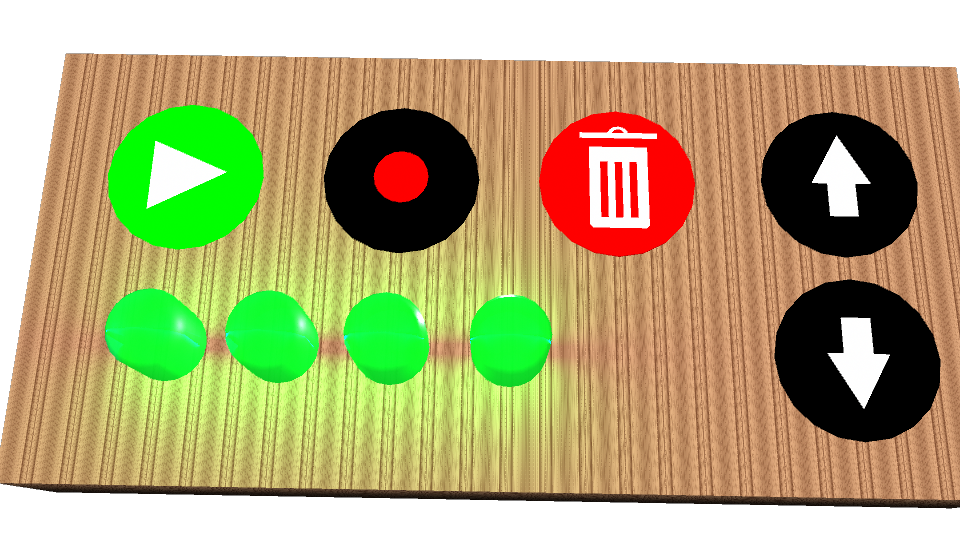
\includegraphics[width=0.7\linewidth]{figure/Design/buttonDesign}
	\label{fig:buttonDesign}
	\caption{Text goes here.}	
\end{figure}

\begin{figure}[H]
	\centering
	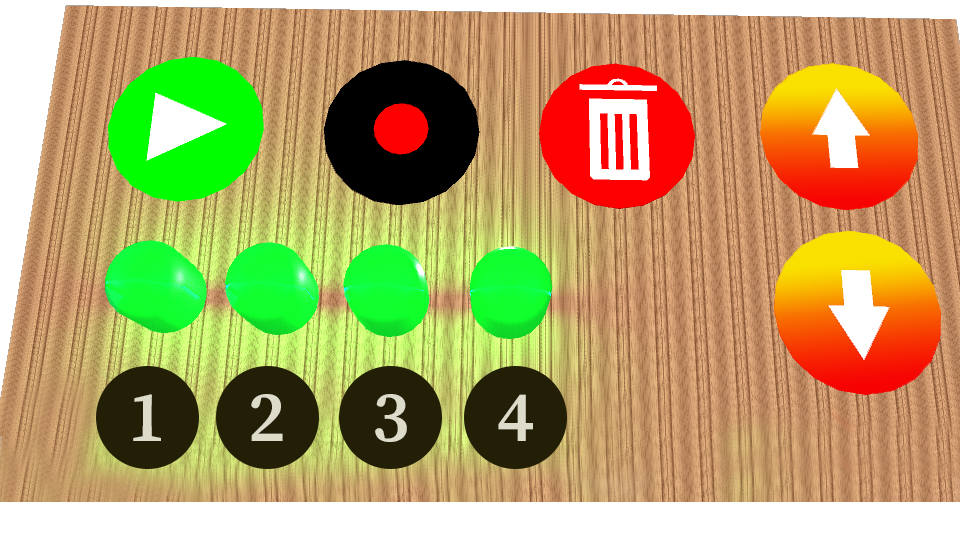
\includegraphics[width=0.7\linewidth]{figure/Design/buttonDesign2}
	\label{fig:buttonDesign2}
	\caption{Text goes here.}	
\end{figure}




Visualizing the tool with all of the design decisions made in this chapter, the final design should resemble \autoref{fig:designFinal}.  
\begin{figure}[H]
	\centering
	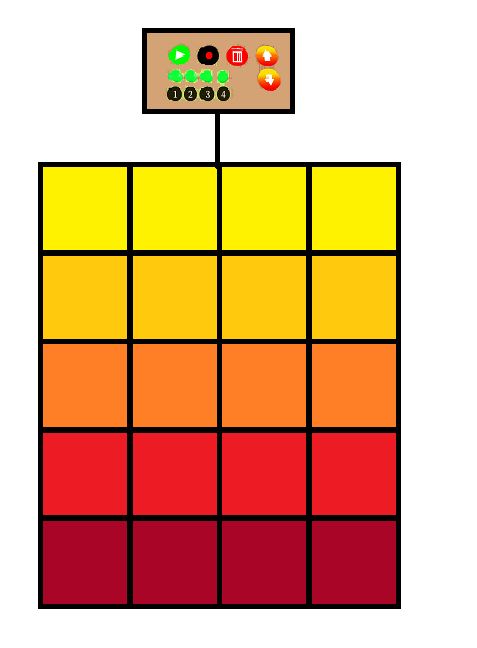
\includegraphics[width=0.7\linewidth]{figure/Design/DesignFinal}
	\label{fig:designFinal}
	\caption{A visualization of the final design.}	
\end{figure}













\section{Testing the design - Usability}
To test the usability of the mat and the control panel on the box a Usability test was conducted. This section explains how this test was prepared and executed. Furthermore, the findings from the test will be described.

\subsection{Preparations of test}
The goal of the test is to determine how usable the prototype is by the users and to eliminate possible challenges that might arise while interacting with the system. By having the test participants complete a few tasks based on some of the use cases, that the prototype was designed for, and by observing how they manage to complete said tasks will indicate how the general usability of the system is and where the prototype is causing problems. To gather concrete data from the test the System Usability Scale(SUS)\cite{susScale} was used. It is a 10-item likert scale that is used to evaluate the usability of any given interactive system with both positively and negatively worded items. Based on prior research item 8 of the SUS-scale was reworded so the word \textit{cumbersome} was replaced by the word \textit{awkward}\cite{susScale}.


\subsection{Location}
The test participants for the usability test were found by convenience sampling around campus on Aalborg University Copenhagen (AAU CPH) as mentioned in \ref{chap:methods}. The participants were brought into a small room either as one person at a time or in pairs. The total number of participants was 10 (2 one-person tests and 4 pairs). The mat had been placed in the middle of the room and two computers were made available for the post test SUS-questionnaire. Furthermore, a moderator and two observers were present. In \autoref{fig:usabilityTest} the layout for the test is presented.

\begin{figure}[H]
	\centering
	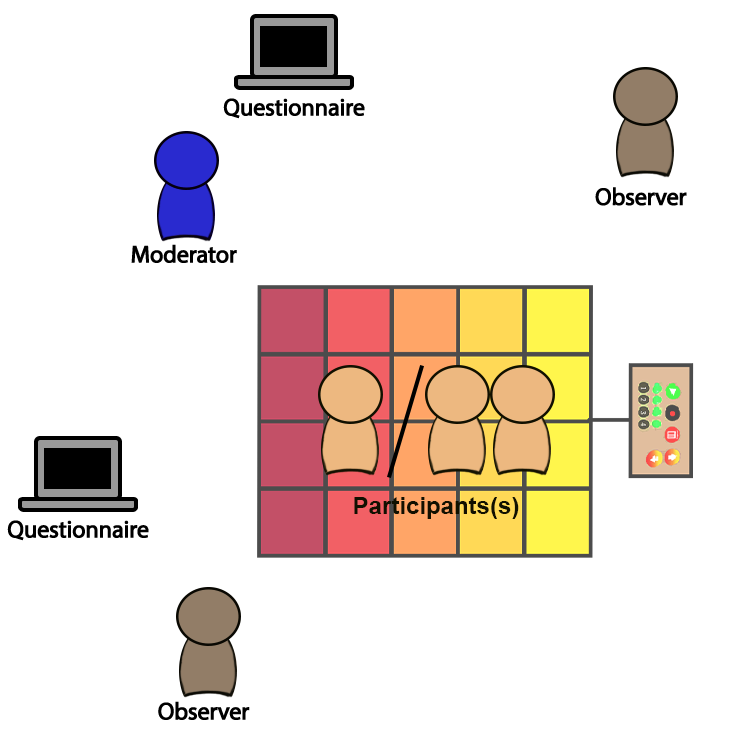
\includegraphics[width=0.7\linewidth]{figure/Design/usability}
	\caption{Figure showing the test layout during the Usability test.}	
	\label{fig:usabilityTest}
\end{figure}

\subsection{Test procedure and observations}

The participants were briefly introduced to the mat and the control panel and were then asked to explore the mat to get a feel of the layout. During this exploration most of the participants quickly discovered the correlation between the color scheme and the tones. They were then asked to change the octaves and this caused some problems. The octave buttons (arrows up and down) were confused with volume buttons and therefore a lot of the participants would try to push the Sequence buttons when asked to octavate. When discovering the octave buttons, sometimes with help from the moderator, the next task was completed with more ease as they were asked to lower the octave again. Afterwards, the participants were asked to record a short sequence and every time they would press the record button and then walk freely around on the mat and try to stop recording by pressing the record button again. When asked to play back what they recorded they would discover that the recording did not sound anything like what they played as the sequencer-like mechanism which makes the mat only record one column/beat at a time was not understood. Finally, they were asked to make sense of the control panel and explain in their own word, what they would expect the different buttons did. The icons on the play, record and delete buttons were self explanatory for most participants, however the sequence buttons were not. There was a lot of different explanations as to what the numbered buttons did e.g. add various filters and effects, change the scale, toggle buttons for enabling/disabling the columns of the mat as the number of columns and the number of sequences were the same. When all the tasks were completed some participants would comment on the lack of indication of which column/beat was playing when they recording. Also, they requested indicators on the control panel to make it more clear what the buttons did. After the test the participants were asked to fill out a SUS-questionnaire on one of the two available computers which was the final part of the usability test.

\subsection{SUS Questionnaire}
In \autoref{fig:susResults} the results from the SUS-questionnaire, that followed the Usability test, are visualized in the form of a box plot graph. The following is a list of the questions from the SUS scale. The odd-numbered items in blue are considered the positively worded questions, whereas the even-numbered items in red are worded negatively. This is relevant for later analysis of the results.\\

\begin{enumerate}
	\item  \textcolor{blue}{I think that I would like to use this system frequently.}
	\item  \textcolor{red}{I found the system unnecessarily complex.}
	\item  \textcolor{blue}{I thought the system was easy to use.}
	\item  \textcolor{red}{I think that I would need the support of a technical person to be able to use this system.}
	\item  \textcolor{blue}{I found the various functions in this system were well integrated.}
	\item  \textcolor{red}{I thought there was too much inconsistency in this system.}
	\item  \textcolor{blue}{I would imagine that most people would learn to use this system very quickly.}
	\item  \textcolor{red}{I found the system very awkward to use.}
	\item  \textcolor{blue}{I felt very confident using the system.}
	\item  \textcolor{red}{I needed to learn a lot of things before I could get going with this system.}
\end{enumerate} 
%SUS boxplot

\begin{figure}[H]
	\centering
	% This file was created by matlab2tikz.
%
%The latest updates can be retrieved from
%  http://www.mathworks.com/matlabcentral/fileexchange/22022-matlab2tikz-matlab2tikz
%where you can also make suggestions and rate matlab2tikz.
%
\begin{tikzpicture}

\begin{axis}[%
width=0.9\linewidth,
height=3.566in,
scale only axis,
unbounded coords=jump,
xmin=0.5,
xmax=10.5,
xtick={1,2,3,4,5,6,7,8,9,10},
xlabel style={font=\color{white!15!black}},
xlabel={Question No.},
ymin=0.257573175810164,
ymax=5.7459492315434,
ylabel style={font=\color{white!15!black}},
ylabel={Level of agreement},
axis background/.style={fill=white},
title style={font=\bfseries},
title={Results from the SUS Questionnaire},
legend style={legend cell align=left, align=left, draw=white!15!black}
]
\addplot [color=black, dashed, forget plot]
  table[row sep=crcr]{%
1	2\\
1	3\\
};
\addplot [color=black, dashed, forget plot]
  table[row sep=crcr]{%
2	3\\
2	4\\
};
\addplot [color=black, dashed, forget plot]
  table[row sep=crcr]{%
3	5\\
3	5\\
};
\addplot [color=black, dashed, forget plot]
  table[row sep=crcr]{%
4	3\\
4	4\\
};
\addplot [color=black, dashed, forget plot]
  table[row sep=crcr]{%
5	4\\
5	4\\
};
\addplot [color=black, dashed, forget plot]
  table[row sep=crcr]{%
6	2\\
6	2\\
};
\addplot [color=black, dashed, forget plot]
  table[row sep=crcr]{%
7	5\\
7	5\\
};
\addplot [color=black, dashed, forget plot]
  table[row sep=crcr]{%
8	4\\
8	5\\
};
\addplot [color=black, dashed, forget plot]
  table[row sep=crcr]{%
9	4\\
9	5\\
};
\addplot [color=black, dashed, forget plot]
  table[row sep=crcr]{%
10	3\\
10	5\\
};
\addplot [color=black, dashed, forget plot]
  table[row sep=crcr]{%
1	1\\
1	1\\
};
\addplot [color=black, dashed, forget plot]
  table[row sep=crcr]{%
2	1\\
2	1\\
};
\addplot [color=black, dashed, forget plot]
  table[row sep=crcr]{%
3	2\\
3	3\\
};
\addplot [color=black, dashed, forget plot]
  table[row sep=crcr]{%
4	1\\
4	1\\
};
\addplot [color=black, dashed, forget plot]
  table[row sep=crcr]{%
5	4\\
5	4\\
};
\addplot [color=black, dashed, forget plot]
  table[row sep=crcr]{%
6	2\\
6	2\\
};
\addplot [color=black, dashed, forget plot]
  table[row sep=crcr]{%
7	3\\
7	4\\
};
\addplot [color=black, dashed, forget plot]
  table[row sep=crcr]{%
8	1\\
8	2\\
};
\addplot [color=black, dashed, forget plot]
  table[row sep=crcr]{%
9	1\\
9	2\\
};
\addplot [color=black, dashed, forget plot]
  table[row sep=crcr]{%
10	1\\
10	1\\
};
\addplot [color=black, forget plot]
  table[row sep=crcr]{%
0.875	3\\
1.125	3\\
};
\addplot [color=black, forget plot]
  table[row sep=crcr]{%
1.875	4\\
2.125	4\\
};
\addplot [color=black, forget plot]
  table[row sep=crcr]{%
2.875	5\\
3.125	5\\
};
\addplot [color=black, forget plot]
  table[row sep=crcr]{%
3.875	4\\
4.125	4\\
};
\addplot [color=black, forget plot]
  table[row sep=crcr]{%
4.875	4\\
5.125	4\\
};
\addplot [color=black, forget plot]
  table[row sep=crcr]{%
5.875	2\\
6.125	2\\
};
\addplot [color=black, forget plot]
  table[row sep=crcr]{%
6.875	5\\
7.125	5\\
};
\addplot [color=black, forget plot]
  table[row sep=crcr]{%
7.875	5\\
8.125	5\\
};
\addplot [color=black, forget plot]
  table[row sep=crcr]{%
8.875	5\\
9.125	5\\
};
\addplot [color=black, forget plot]
  table[row sep=crcr]{%
9.875	5\\
10.125	5\\
};
\addplot [color=black, forget plot]
  table[row sep=crcr]{%
0.875	1\\
1.125	1\\
};
\addplot [color=black, forget plot]
  table[row sep=crcr]{%
1.875	1\\
2.125	1\\
};
\addplot [color=black, forget plot]
  table[row sep=crcr]{%
2.875	2\\
3.125	2\\
};
\addplot [color=black, forget plot]
  table[row sep=crcr]{%
3.875	1\\
4.125	1\\
};
\addplot [color=black, forget plot]
  table[row sep=crcr]{%
4.875	4\\
5.125	4\\
};
\addplot [color=black, forget plot]
  table[row sep=crcr]{%
5.875	2\\
6.125	2\\
};
\addplot [color=black, forget plot]
  table[row sep=crcr]{%
6.875	3\\
7.125	3\\
};
\addplot [color=black, forget plot]
  table[row sep=crcr]{%
7.875	1\\
8.125	1\\
};
\addplot [color=black, forget plot]
  table[row sep=crcr]{%
8.875	1\\
9.125	1\\
};
\addplot [color=black, forget plot]
  table[row sep=crcr]{%
9.875	1\\
10.125	1\\
};
\addplot [color=blue, forget plot]
  table[row sep=crcr]{%
0.75	1\\
0.75	2\\
1.25	2\\
1.25	1\\
0.75	1\\
};
\addplot [color=blue, forget plot]
  table[row sep=crcr]{%
1.75	1\\
1.75	3\\
2.25	3\\
2.25	1\\
1.75	1\\
};
\addplot [color=blue, forget plot]
  table[row sep=crcr]{%
2.75	3\\
2.75	5\\
3.25	5\\
3.25	3\\
2.75	3\\
};
\addplot [color=blue, forget plot]
  table[row sep=crcr]{%
3.75	1\\
3.75	3\\
4.25	3\\
4.25	1\\
3.75	1\\
};
\addplot [color=blue, forget plot]
  table[row sep=crcr]{%
4.75	4\\
4.75	4\\
5.25	4\\
5.25	4\\
4.75	4\\
};
\addplot [color=blue, forget plot]
  table[row sep=crcr]{%
5.75	2\\
5.75	2\\
6.25	2\\
6.25	2\\
5.75	2\\
};
\addplot [color=blue, forget plot]
  table[row sep=crcr]{%
6.75	4\\
6.75	5\\
7.25	5\\
7.25	4\\
6.75	4\\
};
\addplot [color=blue, forget plot]
  table[row sep=crcr]{%
7.75	2\\
7.75	4\\
8.25	4\\
8.25	2\\
7.75	2\\
};
\addplot [color=blue, forget plot]
  table[row sep=crcr]{%
8.75	2\\
8.75	4\\
9.25	4\\
9.25	2\\
8.75	2\\
};
\addplot [color=blue, forget plot]
  table[row sep=crcr]{%
9.75	1\\
9.75	3\\
10.25	3\\
10.25	1\\
9.75	1\\
};
\addplot [color=red, forget plot]
  table[row sep=crcr]{%
0.75	2\\
1.25	2\\
};
\addplot [color=red, forget plot]
  table[row sep=crcr]{%
1.75	2\\
2.25	2\\
};
\addplot [color=red, forget plot]
  table[row sep=crcr]{%
2.75	4\\
3.25	4\\
};
\addplot [color=red, forget plot]
  table[row sep=crcr]{%
3.75	3\\
4.25	3\\
};
\addplot [color=red, forget plot]
  table[row sep=crcr]{%
4.75	4\\
5.25	4\\
};
\addplot [color=red, forget plot]
  table[row sep=crcr]{%
5.75	2\\
6.25	2\\
};
\addplot [color=red, forget plot]
  table[row sep=crcr]{%
6.75	5\\
7.25	5\\
};
\addplot [color=red, forget plot]
  table[row sep=crcr]{%
7.75	2\\
8.25	2\\
};
\addplot [color=red, forget plot]
  table[row sep=crcr]{%
8.75	4\\
9.25	4\\
};
\addplot [color=red, forget plot]
  table[row sep=crcr]{%
9.75	1.5\\
10.25	1.5\\
};
\addplot [color=black, draw=none, mark=+, mark options={solid, red}, forget plot]
  table[row sep=crcr]{%
nan	nan\\
};
\addplot [color=black, draw=none, mark=+, mark options={solid, red}, forget plot]
  table[row sep=crcr]{%
nan	nan\\
};
\addplot [color=black, draw=none, mark=+, mark options={solid, red}, forget plot]
  table[row sep=crcr]{%
nan	nan\\
};
\addplot [color=black, draw=none, mark=+, mark options={solid, red}, forget plot]
  table[row sep=crcr]{%
nan	nan\\
};
\addplot [color=black, draw=none, mark=+, mark options={solid, red}, forget plot]
  table[row sep=crcr]{%
5	3\\
5	3\\
5	5\\
5	5\\
};
\addplot [color=black, draw=none, mark=+, mark options={solid, red}, forget plot]
  table[row sep=crcr]{%
6	1\\
6	1\\
6	4\\
6	4\\
};
\addplot [color=black, draw=none, mark=+, mark options={solid, red}, forget plot]
  table[row sep=crcr]{%
7	2\\
};
\addplot [color=black, draw=none, mark=+, mark options={solid, red}, forget plot]
  table[row sep=crcr]{%
nan	nan\\
};
\addplot [color=black, draw=none, mark=+, mark options={solid, red}, forget plot]
  table[row sep=crcr]{%
nan	nan\\
};
\addplot [color=black, draw=none, mark=+, mark options={solid, red}, forget plot]
  table[row sep=crcr]{%
nan	nan\\
};
\end{axis}
\end{tikzpicture}%
	\caption{Figure showing the results of the SUS-questionnaire. The question numbers on the x-axis correspond to the question numbers in the above list of SUS-items}	
	\label{fig:susResults}
\end{figure}

\subsection{Findings}

$$( (Q_1+Q_3+Q_5+Q_7+Q_9)-5+25-(Q_2+Q_4+Q_6+Q_8+Q_{10}) )*2.5$$

\begin{table}[]
	\centering
	\caption{Table showing the SUS score for each individual test participants and the overall mean score. For full table see appendix \ref{appendix:susResults}}
	\label{tab:susScoreTableAppendix}
	\begin{tabular}{|c|c|l|l|}
		\hline
		Participant & SUS Score \\ \hline
		1           & 52.5      \\ \hline
		2           & 75.0      \\ \hline
		3           & 45.0      \\ \hline
		4           & 55.0      \\ \hline
		5           & 75.0      \\ \hline
		6           & 37.5      \\ \hline
		7           & 70.0      \\ \hline
		8           & 80.0      \\ \hline
		9           & 70.0      \\ \hline
		10          & 75.0      \\ \hline
		Total       & 63.5      \\ \hline
	\end{tabular}
\end{table}

\begin{figure}[H]
	\centering
	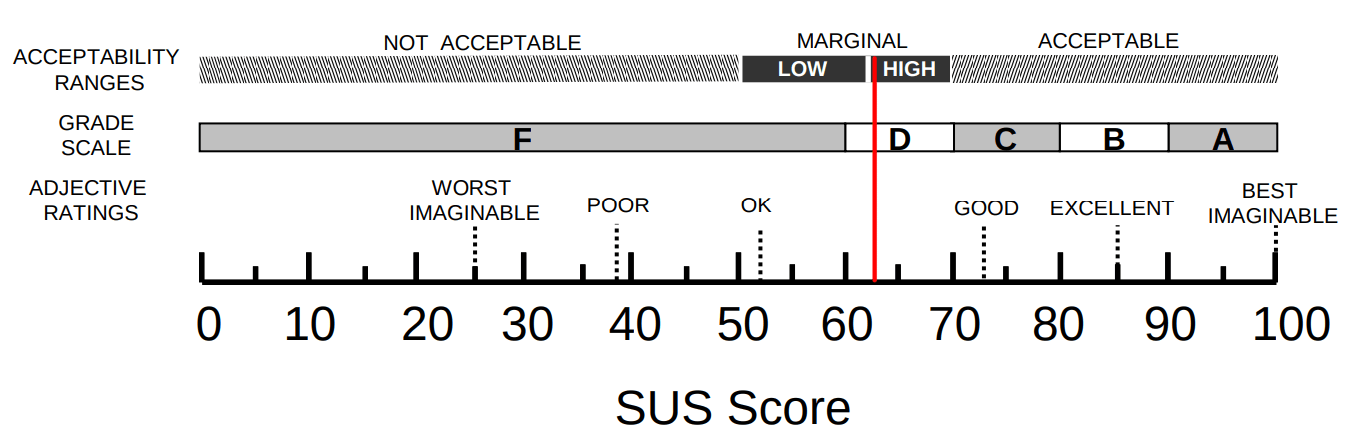
\includegraphics[width=1\linewidth]{figure/Design/susScore}
	\caption{Figure highlighting the test score(63.5) on a scale representing SUS scores and their meanings\cite{susScore}}
	\label{fig:susScore}
\end{figure}

\todo{add conclusion/summary}


\section{Improvements to the final design}
 %  LED og klistermærker 
\todo{kan først skrives når usability er færdig da der skal refereres meget dertil :) }


% IMPLEMENTION
\chapter{Implementation}%Jens
Due to the agile nature of the prototype development the implementation stage begun while the design phase was still underway. This chapter describes what went into the implementation of the final prototype.

\section{Micro controllers}%Daniel
	Initially doing the implementation phase, research went into what kind of micro controller, if any, we would need to construct a working prototype. Initially we settled for an Arduino Mega 2560, but going into the production phase, we realized that an external sound source was needed. The Beaglebone Black with the Bela shield suited this purpose, and was taken in during this process.
	\subsection{Arduino}%Daniel
		The Arduino devices are a small, but versatile group of micro controller, used around the world for DIY projects\todo{Find cite}. The Arduino Mega, with the ATMEGA2560 chip is one of the more powerful variants, with a bigger EEPROM and more pins than the more commonly seen Arduino Uno. The pin amount was paramount in the decision to what micro controller was needed to control the physical interface, as the design called for a 4x5 grid of fields that should be individually activated. 
		
	\subsection{Bela}%Jens
		Due to the sound related limitations from the Arduino Mega, we decided to add a connection to a Beaglebone with a Bela shield\footnote{Bela website: \url{https://bela.io/}}. The Bela provides a broad span of audio processing opportunities to create and manipulate audio as it is compatible with Pure Data(PD). PD is a visual programming language for multimedia that can also be used to create sounds.
	
\section{Code}
	When designing the system for the mat, it came down to three requirements:
	\begin{itemize}
		\item[-] It should be able to save the activated fields in each of the four beats (lines).
		\item[-] It should be able to save the sequences of fields in four separate segments.
		\item[-] It should be able to play back the previously saved segments.
	\end{itemize}
	\subsection{C/C++}%Daniel
		
		To categorize the data and prepare it for saving on the Mega, two separate structures where made. These structures as seen in \autoref{listing:structs} are called \mintinline{cpp}{SequenceField} and \mintinline{cpp}{Segment}. SequenceField contains an \mintinline{cpp}{int} that holds the octave of the sequence, and a \mintinline{cpp}{Field} array to hold the activated fields.
		
		\noindent
		The \mintinline{cpp}{Segment} structure holds a \mintinline{cpp}{SequenceField} array to contain the 4 sequences (beats), a \mintinline{cpp}{bool} to keep track of what segment is enabled, and the corresponding LED pin.
		
		\begin{listing}[H]
			\caption{The structs used to contain our data for the segments and their fields.}
			\label{listing:structs}
			\begin{minted}[frame=lines,framesep=2mm,baselinestretch=1.1,fontsize=\footnotesize,linenos]{cpp}
struct SequenceField {
  int octave = 4;
  Field activatedFields[5];
};

struct Segment {
  bool enabled = true;
  int ledPin;
  SequenceField sequence[4];
};
			\end{minted}
		\end{listing}
		\noindent
		To save the segments and their data to persist through restarts, we make use of the onboard EEPROM. The EEPROM on the Arduino Mega can hold 4k bytes of data and our segments only take up 611 bytes of that space. Writing to the EEPROM on an Arduino is quite straightforward, we simply iterate over our \mintinline{cpp}{Segment} array, and put in into the EEPROM according to the size of our structure.
		\begin{listing}[H]
			\caption{Writing our segment data to the EEPROM}
			\label{listing:writeSegment}
			\begin{minted}[frame=lines,framesep=2mm,baselinestretch=1.1,fontsize=\footnotesize,linenos]{cpp}
void writeSegments() {
  for(int i = 0; i < amountOfSegments; i++) {
	EEPROM.put(i*sizeof(Segment), segments[i]);
  }
}
			\end{minted}
		\end{listing}
		\noindent
		\autoref{fig:flowchartPlayRecord} explains what happens when either the record or play buttons is pressed. Pressing the play button, goes through the enabled segments, and plays the sequences in each. Pressing the record button however starts a more complex routine, starting with going over each field in the current beat and checking if it's activated. Then an empty Field object is made for each field, to record silence in the fields where no kid were standing. If a field was activated, then it saves the octave in the sequence and the field in \mintinline{cpp}{activatedFields[]}. In the end it plays the activated fields' sounds.
		\begin{figure}[H]
			\centering
			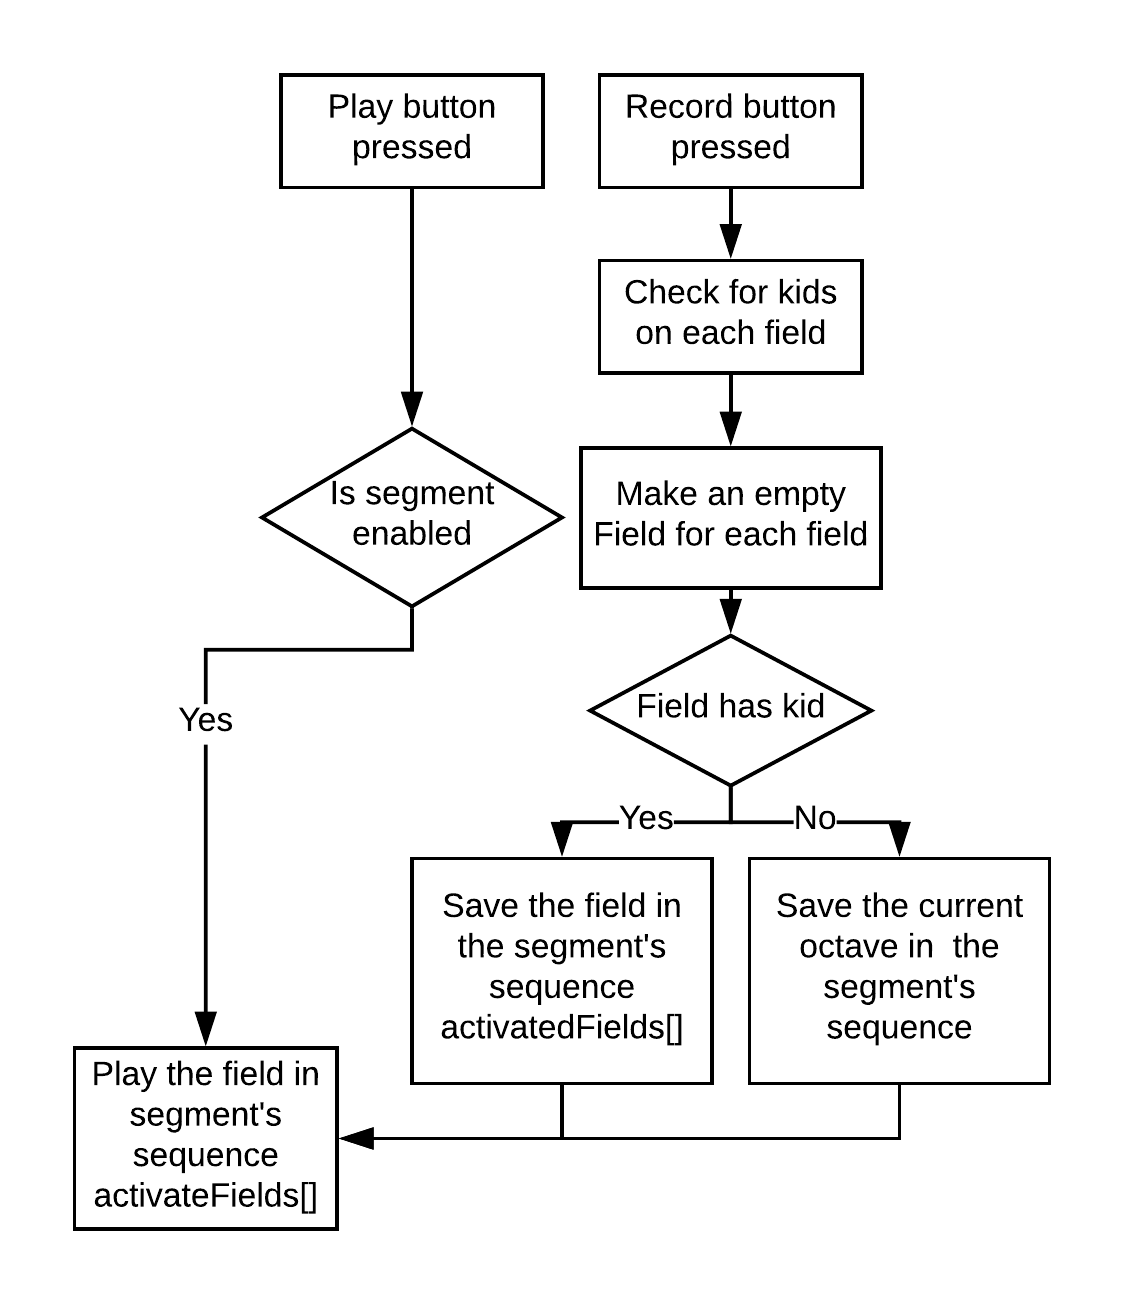
\includegraphics[width=.5\linewidth]{figure/Implementation/flowchartPlayRecord}
			\caption{Flowchart of pressing either the play or record button}
			\label{fig:flowchartPlayRecord}
			\end{figure}
	
		\subsubsection{Libraries}%Daniel
			To achieve some of the functionality in a short amount of time, two libraries were used in addition to our own system,
			the FastLed and Button library. The button library is fairly self explanatory, it is library with a button class, that makes it easy to read button presses and account for debounce. The FastLed library makes it easy to interface with and control a LED strip or LED matrix.
	\subsection{PureData}%Jens
		\autoref{fig:pdPatch} shows the main patch of the PD code that was uploaded to the Bela. It takes inputs through the Belas' pins from the Arduino Mega. The PD patch is responsible for playing the sounds when the pads are pressed, changing the octave by multiplying/dividing the oscillators' frequencies by 2, playing the count in sound before recording or playing.
	
	\begin{figure}[H]
		\centering
		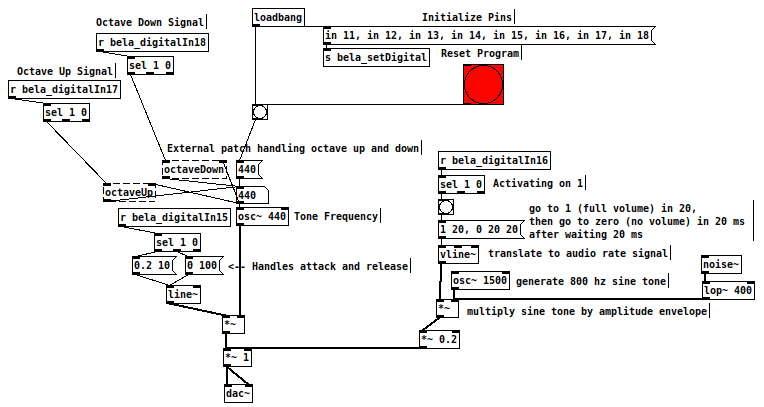
\includegraphics[width=1\linewidth]{figure/Implementation/pureDataPatch}
		\caption{Figure showing the main Pure Data patch for the prototype}
		\label{fig:pdPatch}
	\end{figure}
	\noindent
	Due to the 4x5 layout of the mat, and the 4 was representing 4 beats, there was a need for a scale that would fit 5 tones. Therefore a pentatonic scale was chosen. It consists of 5 tones and therefore 5 frequencies. These were generated by an Oscillator object. A functionality for octavating the scale up and down was implemented to add more variety and opportunity. By dividing the current tone frequency by 2 the octave is lowered and by multiplying by 2 it is raised. \autoref{tab:toneFreq} shows a table of the frequencies for the octaves available on the system.
	
	\begin{table}[H]
		\centering
		\caption{Table showing the oscillator tone frequencies for the pentatonic scales in the different octaves.}
		\label{tab:toneFreq}
		\begin{tabular}{|c|c|c|c|c|c|}
			\hline
			Octave/tones & C     & D     & E     & G    & A    \\ \hline
			3            & 130.5 & 146.5 & 164.5 & 196  & 220  \\ \hline
			4            & 261   & 293   & 329   & 392  & 440  \\ \hline
			5            & 522   & 586   & 658   & 784  & 880  \\ \hline
			6            & 1044  & 1172  & 1316  & 1568 & 1760 \\ \hline
		\end{tabular}
	\end{table}
	



\section{The box}%Jens
In order to conceal wires and micro controllers and to construct an easy way of controlling the various features a box was created. This section explains how the control box was built.

	\subsection{CAD}
	Autodesk's Fusion 360\footnote{Product overview page for Fusion 360: \url{https://www.autodesk.com/products/fusion-360/overview}} with an additional box generation plugin provided a convenient way of creating the blueprint for the control box that would later be used to laser cut the 6 sides of the box. Holes were cut onto the lid of the box to be able to place the needed buttons and LEDs (See \autoref{fig:finalbox1}). On the side facing the mat a square hole was cut that would be used for a custom made plug for easily connecting the mat with the Arduino Mega. For decoration a G-clef was also printed onto the front facing side. On the backside holes were cut to provide easy access for adding an external speaker through a female jack plug and also to power the Bela using a USB cable.
	
	
	\begin{figure}[H]
		\centering
		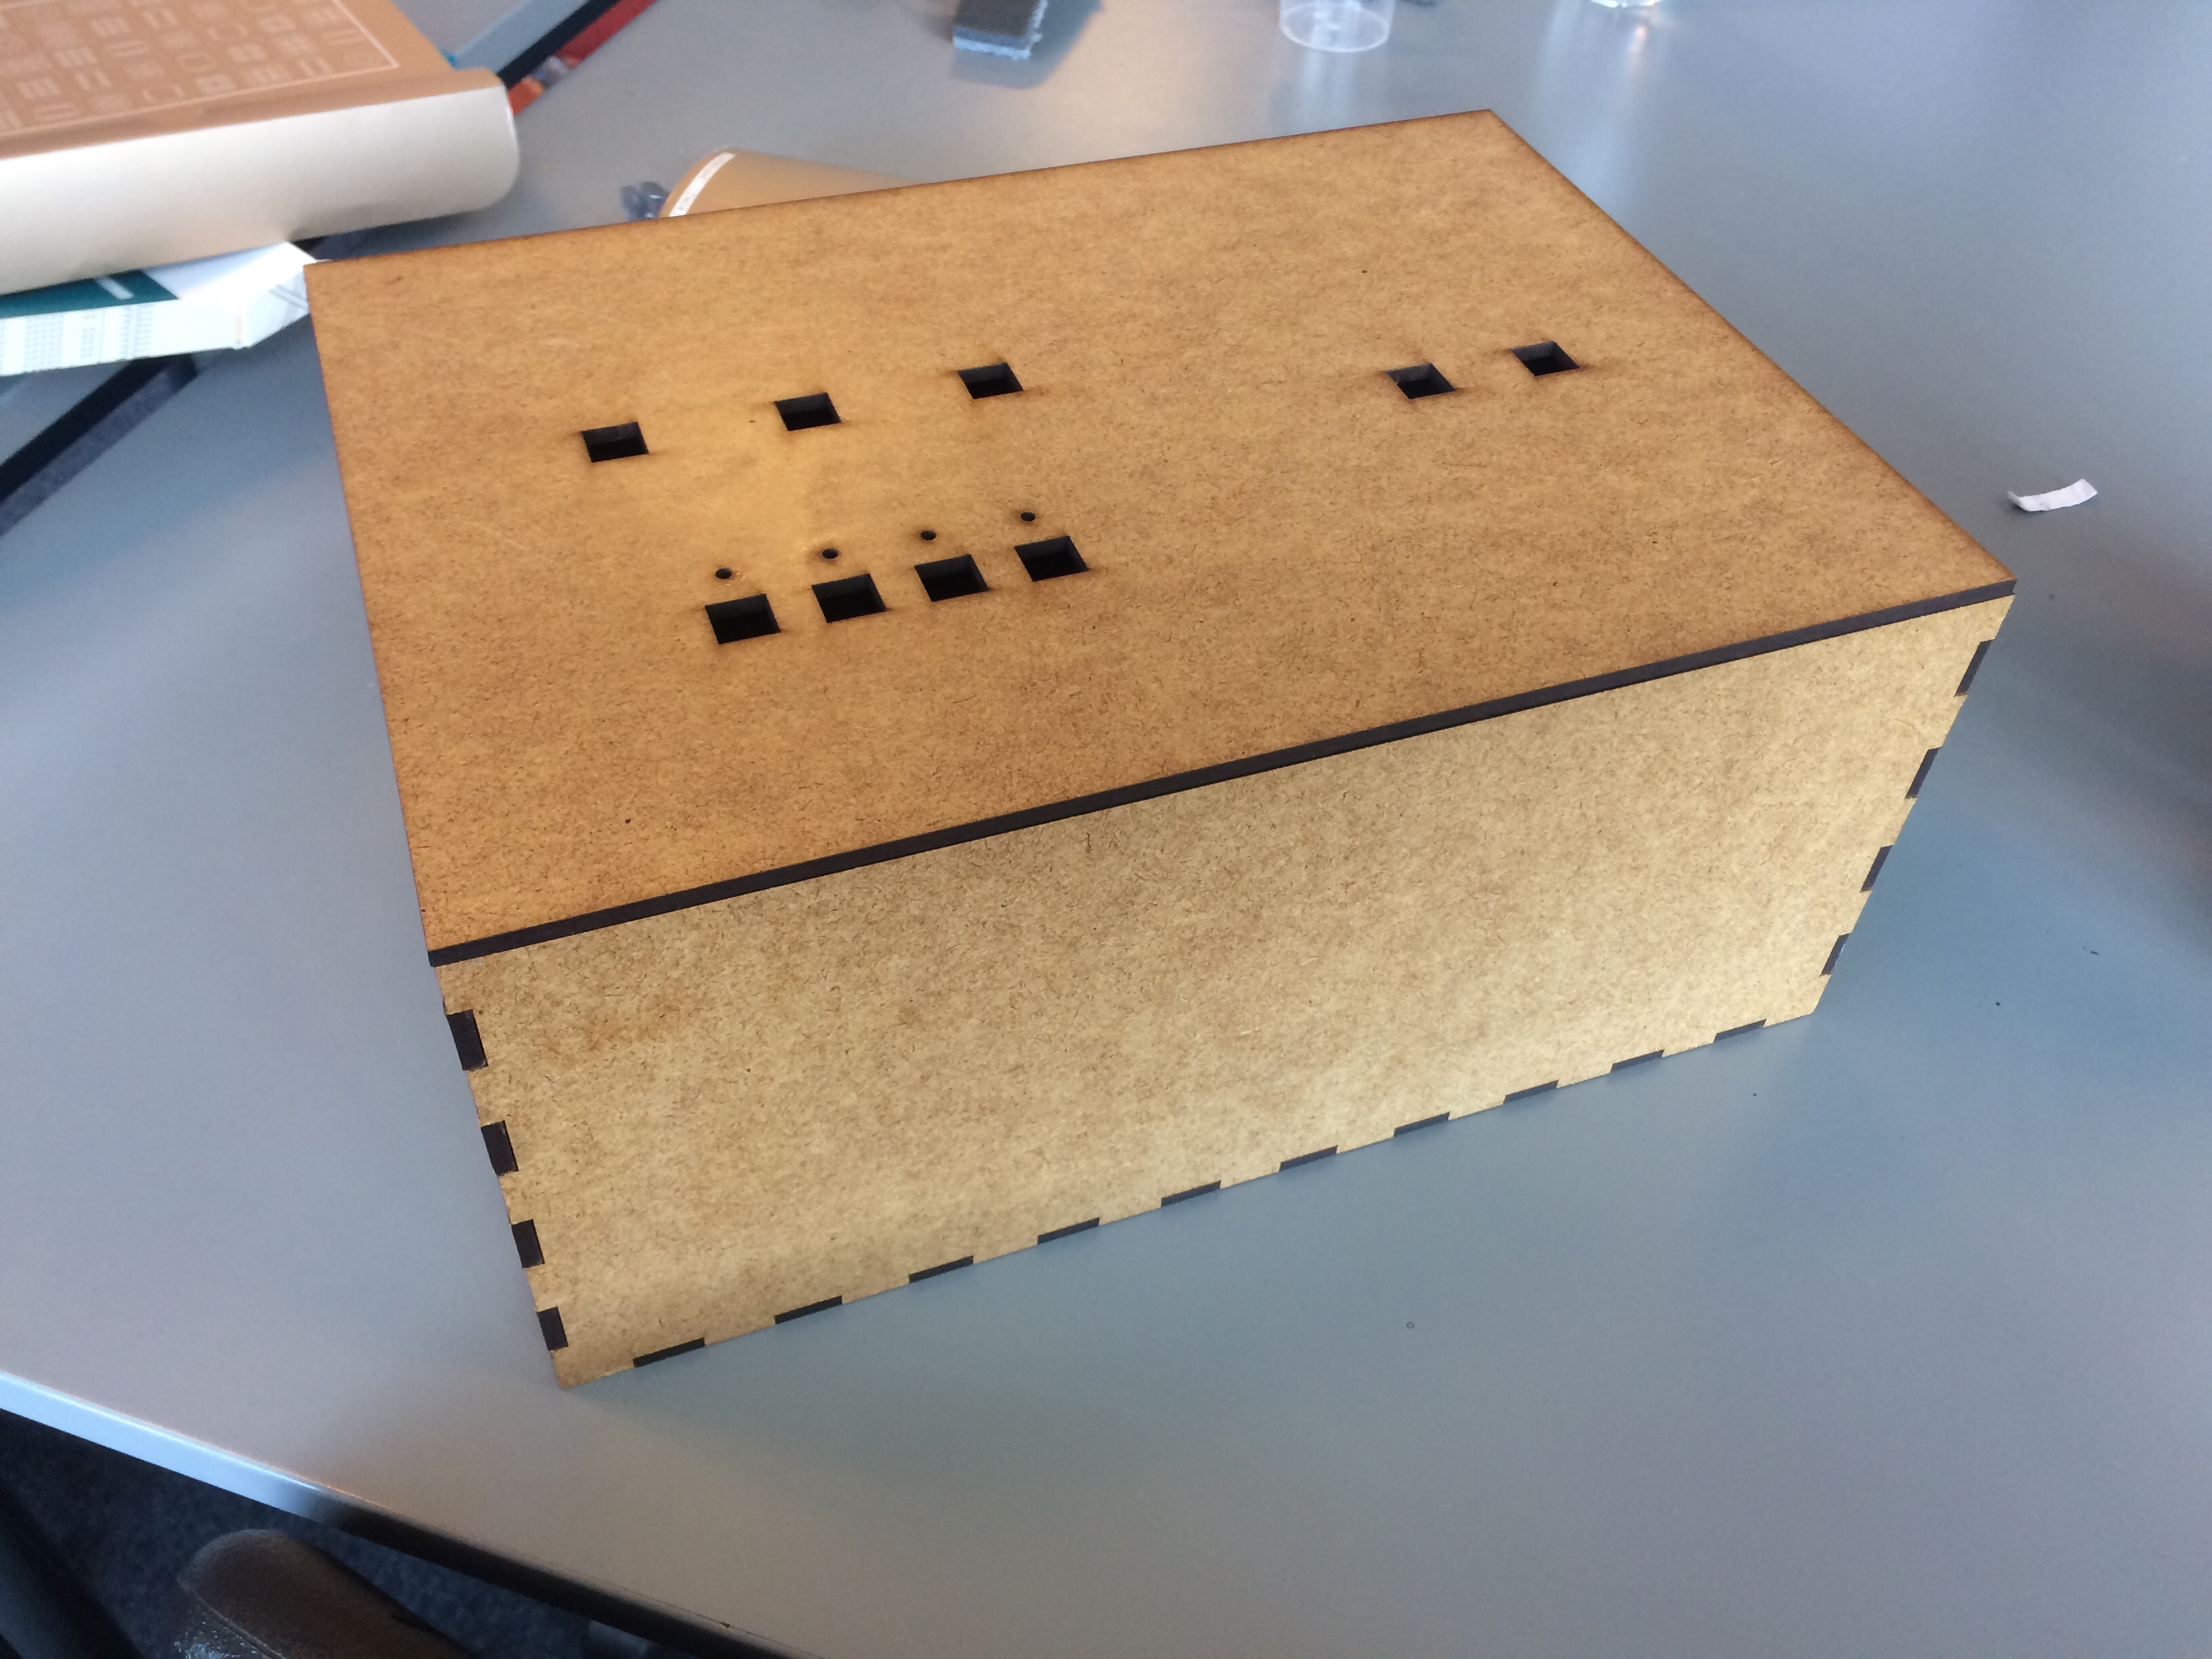
\includegraphics[width=0.7\linewidth]{figure/Design/finalbox1}
		\caption{The final prototype box}	
		\label{fig:finalbox1}
	\end{figure}
	
		
	\subsection{Assembly}
	Due to the way the sides of the box were constructed with finger joints that fit together the box was easy to assemble. With a kerf of 0,275mm the sides were able to stick to each other without using additional glue or nails. However, the plugs were glued to the inside of the box. This was also the case for the buttons and the LEDs on the lid. These also required wires that were soldered on with extra length which made it possible to lift the lid of the box without wires being detached from the micro controllers. Within the lid a frame was glued on to hold the lid in place since the lid was not made with joints (See \autoref{fig:finalbox2}).
	
		\begin{figure}[H]
			\centering
			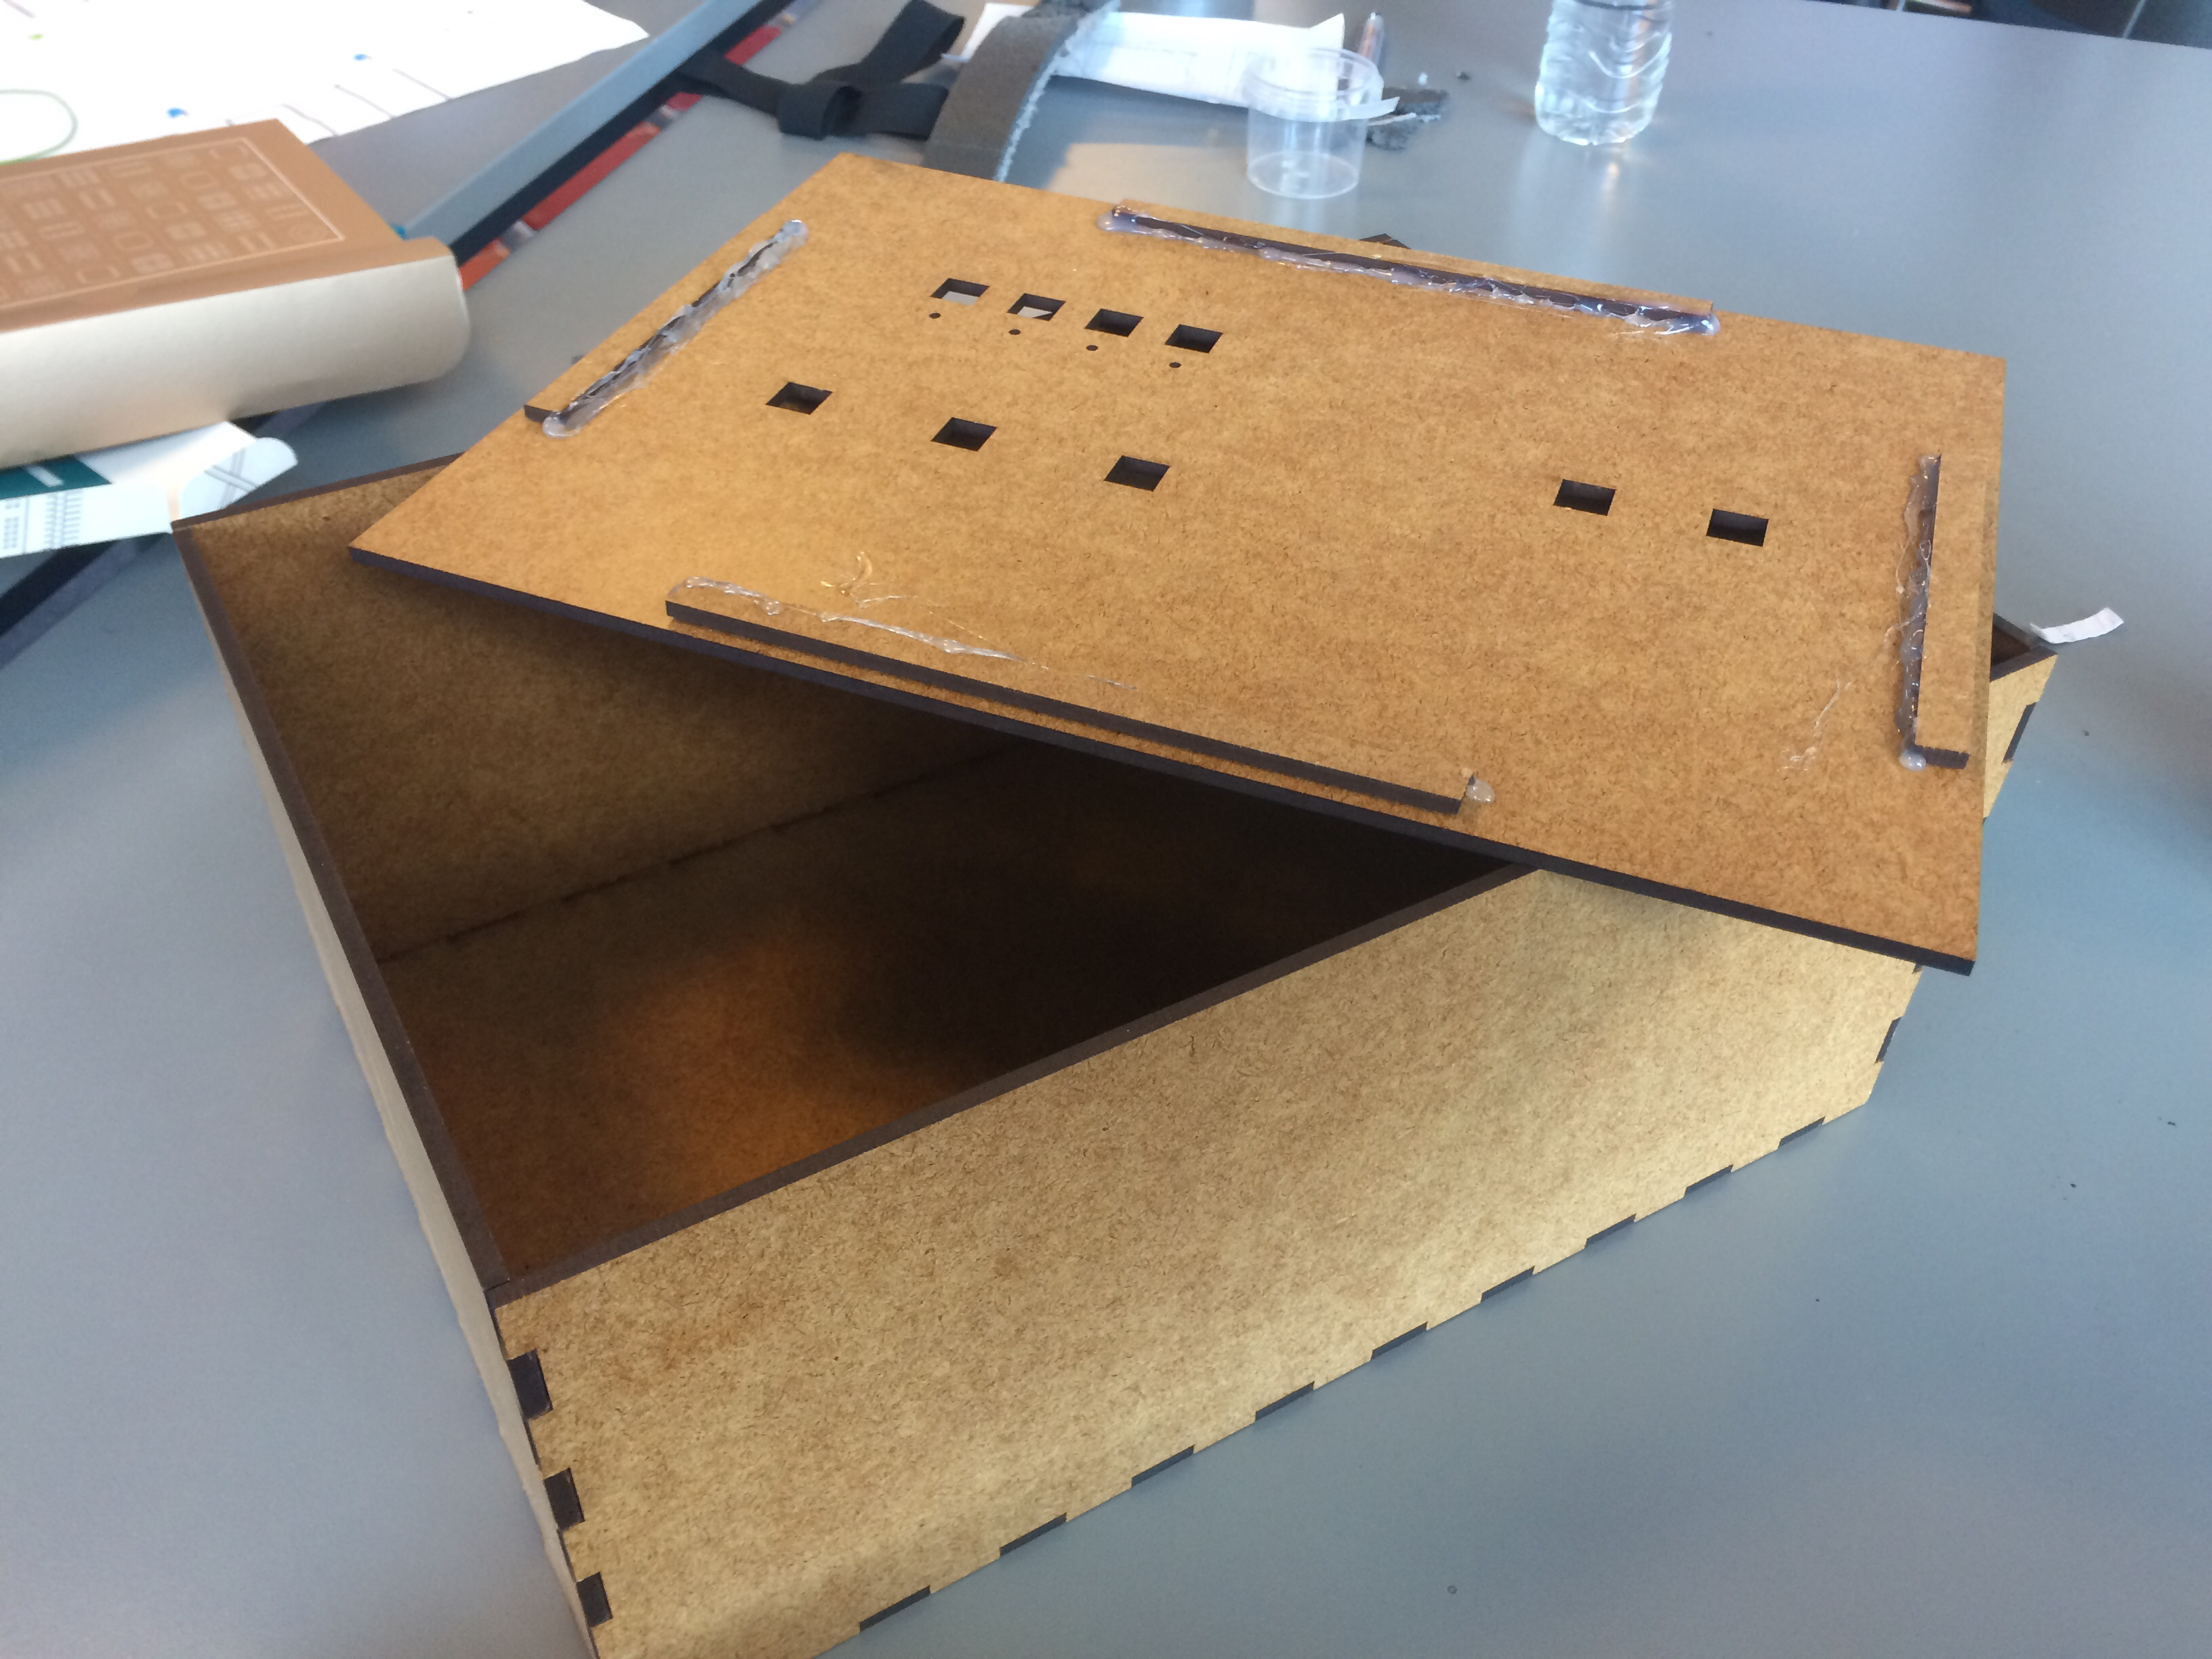
\includegraphics[width=0.7\linewidth]{figure/Design/finalbox2}
			\caption{The final prototype box}
			\label{fig:finalbox2}
		\end{figure}
		
		\begin{figure}[H]
			\centering
			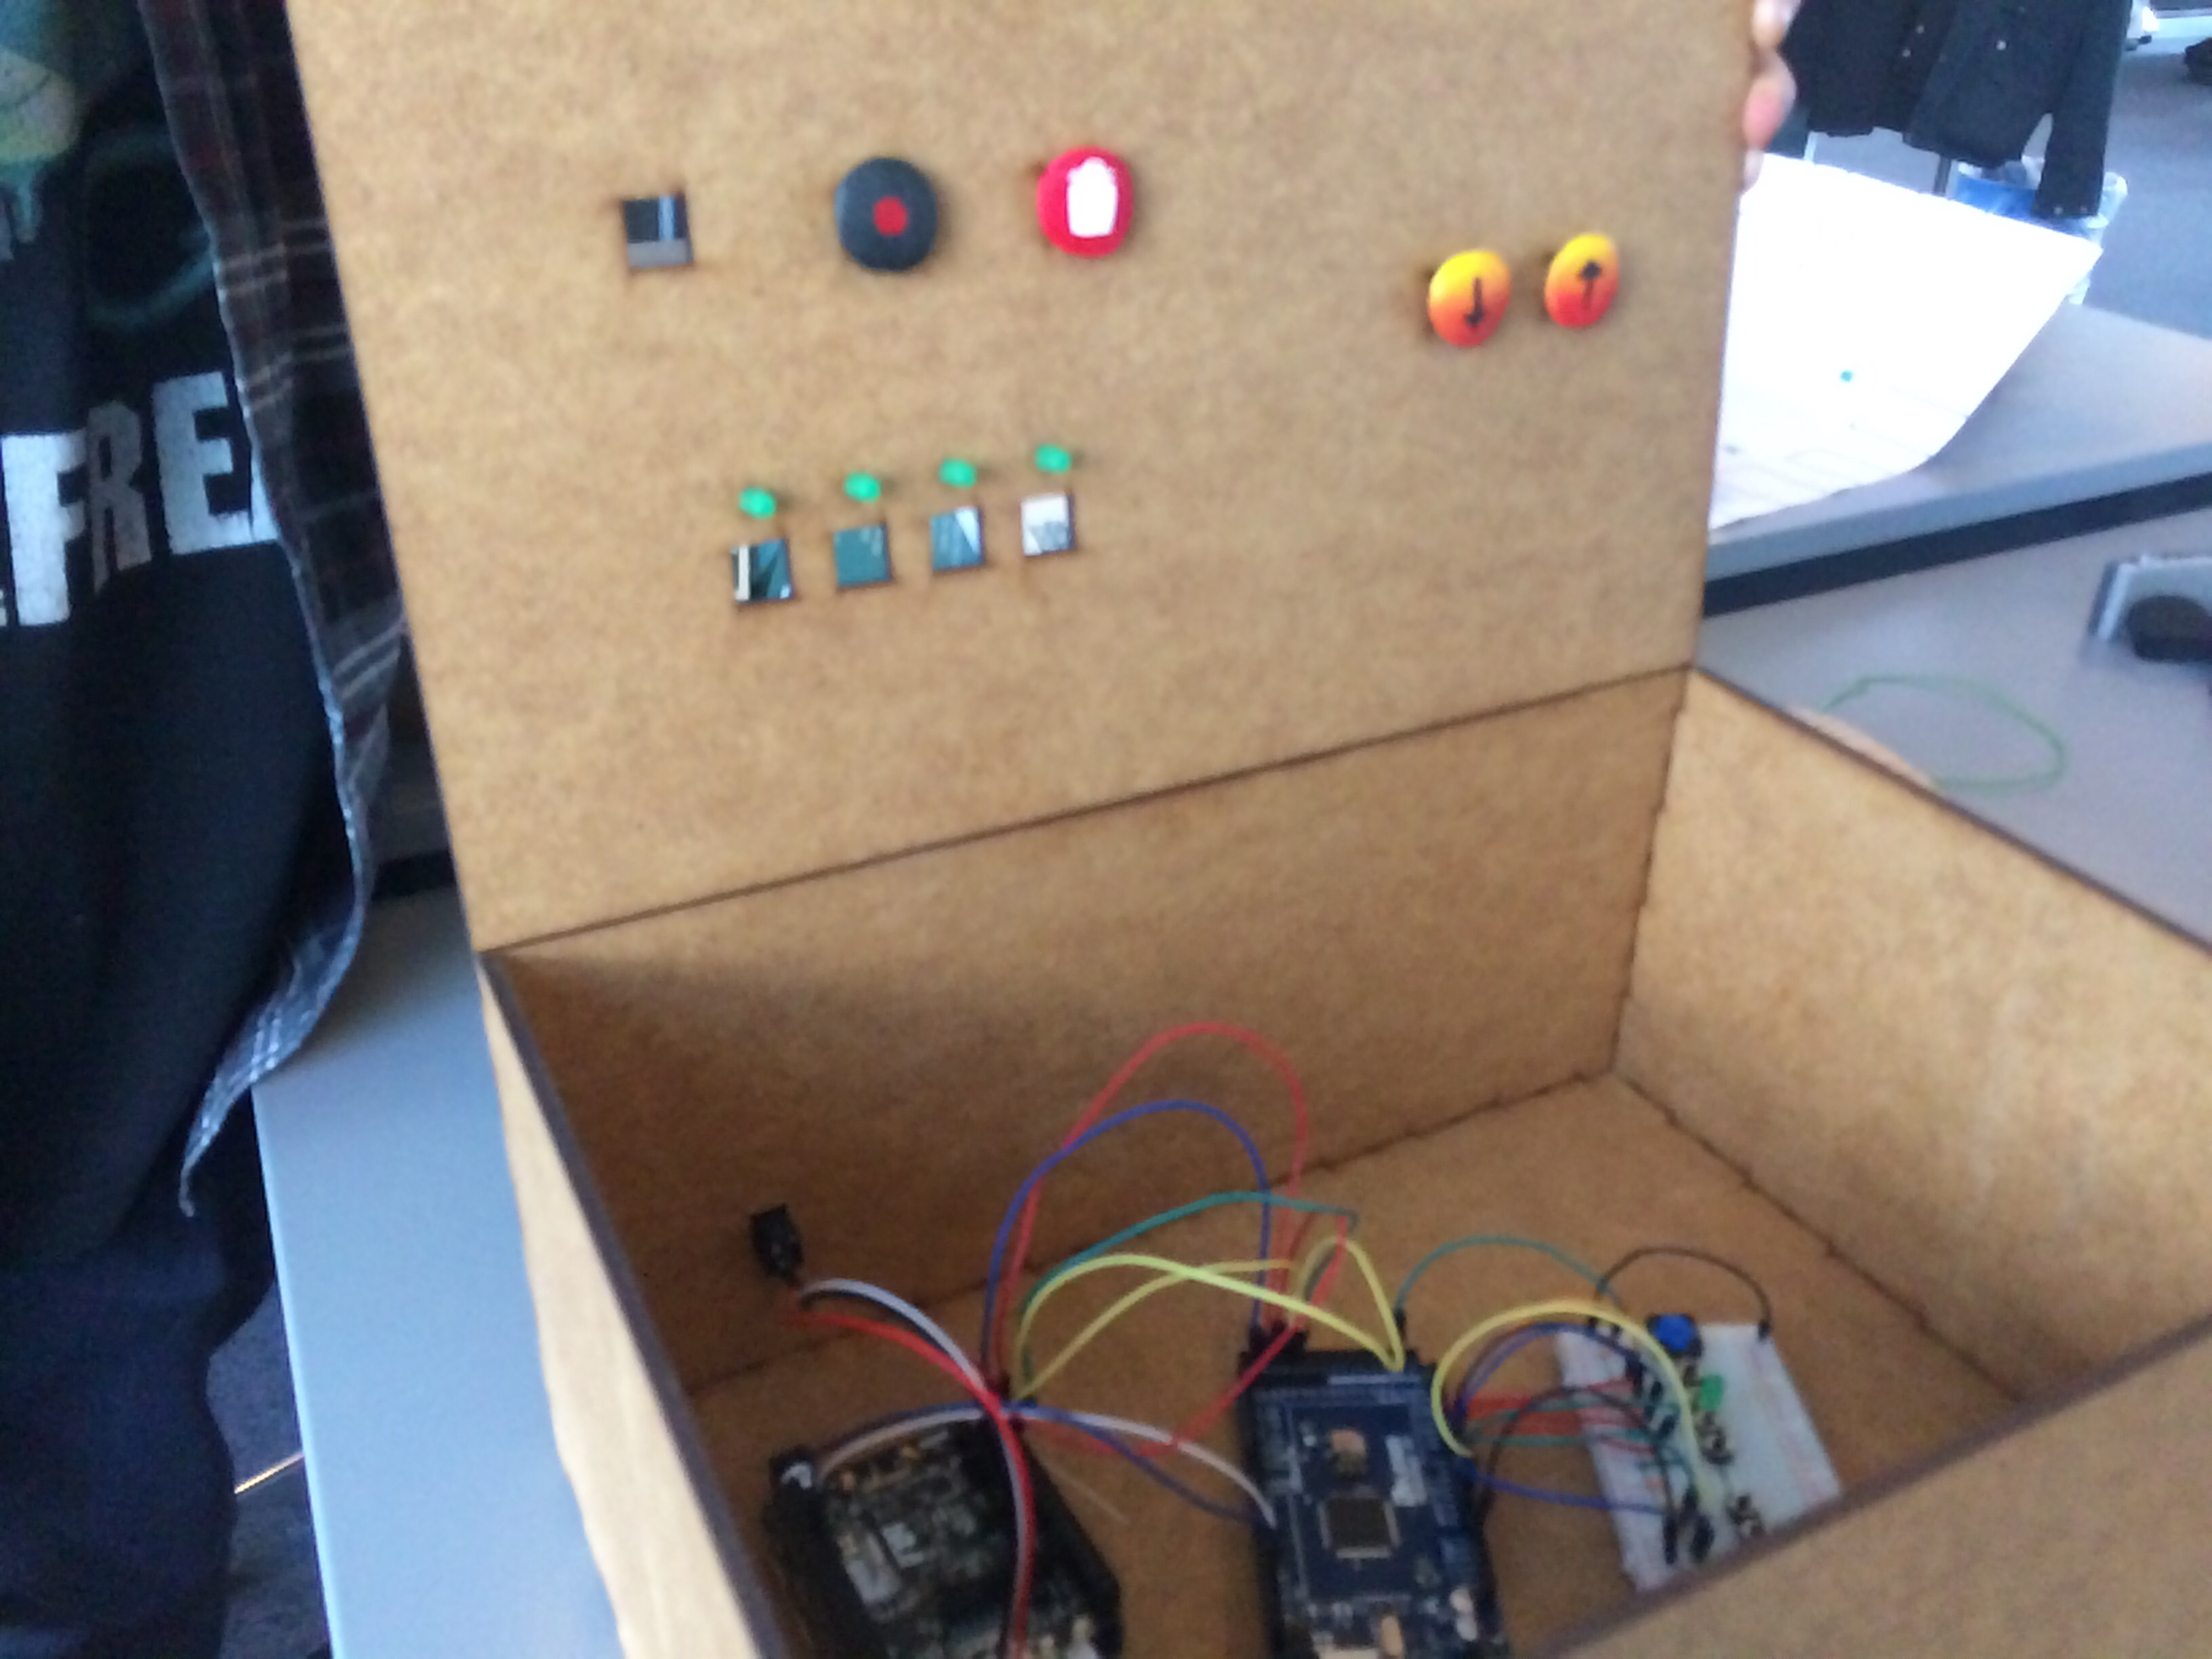
\includegraphics[width=0.7\linewidth]{figure/Design/finalbox3}
			\caption{The final prototype box with the electronic components inside}
			\label{fig:finalbox3}
		\end{figure}

\section{The mat}%Daniel

\section{Circuit}

% Evaluation
\chapter{Evaluation}

The purpose of this chapter is to explain how the final iteration of the prototype was evaluated. The chapter will focus on the evaluation methods used, as well as representing data and discussing the results. The evaluation aimed towards concluding upon the final problem statement, and provide a better understanding about collaboration in groups.\\\\
The final test was conducted on a 4th grade at Skt. Annæ music elementary school. The goal of the test was to gather both quantative data as well as qualitative data. The qualitative test was a observation test, and the quantitative test was a Likert scale. These tests aim towards evaluating the prototype in correlation to the design requirements, as well as answering the final problem statement.

\section{Methods}
This section will describe the methods used in correlation to the methods presented in \autoref{chap:methods}. The section will present both the methods used to conduct the different tests, as well as which methods that has been used to analyse and conclude on the data. 

\subsection{Qualitative Test}
To get a better understanding of how the group collaborates; understanding how the group is using the prototype, and if they form some sort of group roles while using the prototype. To get a better view on the potential group roles, a non-participant test was conducted\ref{bjoernerBog}. Using a non-participant test will prevent the observers from being a part of the test and pottentially making the participants biased. Using this form of interview also creates a symbolisation of how the prototype would be used in a natural settings. A thing to keep in mind when conducting non-participant interviews, is that the data relies heavily on the observers interpretation of the events. Therefore it is important that the observer knows exactly what to look for. In this test, the observers relied heavily on the information gained from the analysis about group roles and collaboration\ref{bjoernerBog}.\\\\
(Insert data crunching method here :))

\subsection{Quantitative Test}
To test whether the test participants found the prototype collaborative or not, a Likert scale was used. The scale ranged from \textit{Disagree Strongly} to \textit{Agree Strongly}. The questions focused on statements which would give insight in how the test participant experienced the prototype in a collaborative manor. For all the questions on the Likert scale see appendix XX \ref{fig:likertScale}. The purpose of the Likert scale was for the participants to answer both positive as well as negative driven statements about differnet parts of collaboration i.e. if they felt that a person had more control than the others, or if they felt that they took part in the activities on the prototype.\\\\
Insert Methods about Likert scale data behandling.

\section{The Test}
As mentioned, the final test was conducted on a 4th grade on the Skt. Annæ music school. The total amount of testers were 25 students,  divided into 5 subgroups. Each group consisting of 5 participants took part in the activities on the prototype. Each group had a an approximate 10-13 minutes on the prototype, and 3-5 minutes filling out the Likert scale afterwards.

\subsection{The Setup}
The test was split up into 2 parts. The first part was where the students was executing the test while being observed. When the participants were lead into the room, they were first of, given a short introduction of how the prototype functions, and what the purpose of the prototype is. Afterwards, the participants were given the task to re-create the melody \textit{Mary Had a Little Lamb}, on the prototype. While playing the tune, the participants were being observed by 2 observers using the non-participant method\ref{bjoernerBog}. \\\\
When the participants completed the tasks, they were taken outside to complete a Likert scale about their collaboration using the prototype. 

Below might need to be sourced

\subsubsection*{Leader/Instructor}
The instructor role was the person that introduced the test participants to the test as well as introduced them to the tasks that the were to conduct. Furthermore, the instructor would answer any general questions, or questions regarding the execution of the test or the tasks. The same person also had a leader role and made sure that the test was conducted acording to plan, and kept time of the test participant. This person would only introduce the prototype and the tasks, while staying out of the test as much as possible to avoid causing biased participants.

\subsubsection*{Observers}
The observers would sit in the back of the room while not talking or interacting with the test participants in any way. They used the non-participant method which means that they are not allowed to take any participation in the test. When the test participant entered the room, they were each given a sticker with a letter and a number on, for the observers to keep track of the different participants. The observers goal was to see if the test participant had patterens in a collaborative sense, while testing the prototype. They would observe factors such as group roles, if a natural leader would take place or everyone attempted to work together equally etc. Furthermore, the testers would observe which type of collaboration, if any, would take place. 

\subsubsection*{Likert Scale Conductor}
After the participants were finished interacting with the prototype, they would be led out of the room to take a Liker scale form. The conductor would hand out the papers and introduce the questions. While the participants being children, the conductor made sure to thouroughly explain each question and answer the participants question if they had any. Furtermore, the conductor would make sure that they did not affect the participants by presenting both positive and negative answers equally.

\subsubsection*{Runner}
The runner would help where help is needed, while the main task was to ready the next group of test participants while the other group were finishing up.\todo{Might be redundant}


\section{Results}
to do\todo{to do}
% This file was created by matlab2tikz.
%
%The latest updates can be retrieved from
%  http://www.mathworks.com/matlabcentral/fileexchange/22022-matlab2tikz-matlab2tikz
%where you can also make suggestions and rate matlab2tikz.
%
\begin{tikzpicture}

\begin{axis}[%
width=4.521in,
height=3.566in,
at={(0.758in,0.481in)},
scale only axis,
unbounded coords=jump,
xmin=0.5,
xmax=8.5,
xtick={1,2,3,4,5,6,7,8},
xlabel style={font=\color{white!15!black}},
xlabel={Question No.},
ymin=0.387875,
ymax=5.219625,
ylabel style={font=\color{white!15!black}},
ylabel={Level of Agreement},
axis background/.style={fill=white},
title style={font=\bfseries},
title={Results from collaboration test (n=25)},
legend style={legend cell align=left, align=left, draw=white!15!black}
]
\addplot [color=black, dashed, forget plot]
  table[row sep=crcr]{%
1	5\\
1	5\\
};
\addplot [color=black, dashed, forget plot]
  table[row sep=crcr]{%
2	5\\
2	5\\
};
\addplot [color=black, dashed, forget plot]
  table[row sep=crcr]{%
3	2.25\\
3	4\\
};
\addplot [color=black, dashed, forget plot]
  table[row sep=crcr]{%
4	4\\
4	5\\
};
\addplot [color=black, dashed, forget plot]
  table[row sep=crcr]{%
5	4\\
5	5\\
};
\addplot [color=black, dashed, forget plot]
  table[row sep=crcr]{%
6	4.25\\
6	5\\
};
\addplot [color=black, dashed, forget plot]
  table[row sep=crcr]{%
7	4\\
7	5\\
};
\addplot [color=black, dashed, forget plot]
  table[row sep=crcr]{%
8	3\\
8	5\\
};
\addplot [color=black, dashed, forget plot]
  table[row sep=crcr]{%
1	3\\
1	4\\
};
\addplot [color=black, dashed, forget plot]
  table[row sep=crcr]{%
2	3\\
2	4\\
};
\addplot [color=black, dashed, forget plot]
  table[row sep=crcr]{%
3	1\\
3	1\\
};
\addplot [color=black, dashed, forget plot]
  table[row sep=crcr]{%
4	2\\
4	3\\
};
\addplot [color=black, dashed, forget plot]
  table[row sep=crcr]{%
5	2\\
5	3\\
};
\addplot [color=black, dashed, forget plot]
  table[row sep=crcr]{%
6	2\\
6	3\\
};
\addplot [color=black, dashed, forget plot]
  table[row sep=crcr]{%
7	1\\
7	2\\
};
\addplot [color=black, dashed, forget plot]
  table[row sep=crcr]{%
8	1\\
8	1\\
};
\addplot [color=black, forget plot]
  table[row sep=crcr]{%
0.875	5\\
1.125	5\\
};
\addplot [color=black, forget plot]
  table[row sep=crcr]{%
1.875	5\\
2.125	5\\
};
\addplot [color=black, forget plot]
  table[row sep=crcr]{%
2.875	4\\
3.125	4\\
};
\addplot [color=black, forget plot]
  table[row sep=crcr]{%
3.875	5\\
4.125	5\\
};
\addplot [color=black, forget plot]
  table[row sep=crcr]{%
4.875	5\\
5.125	5\\
};
\addplot [color=black, forget plot]
  table[row sep=crcr]{%
5.875	5\\
6.125	5\\
};
\addplot [color=black, forget plot]
  table[row sep=crcr]{%
6.875	5\\
7.125	5\\
};
\addplot [color=black, forget plot]
  table[row sep=crcr]{%
7.875	5\\
8.125	5\\
};
\addplot [color=black, forget plot]
  table[row sep=crcr]{%
0.875	3\\
1.125	3\\
};
\addplot [color=black, forget plot]
  table[row sep=crcr]{%
1.875	3\\
2.125	3\\
};
\addplot [color=black, forget plot]
  table[row sep=crcr]{%
2.875	1\\
3.125	1\\
};
\addplot [color=black, forget plot]
  table[row sep=crcr]{%
3.875	2\\
4.125	2\\
};
\addplot [color=black, forget plot]
  table[row sep=crcr]{%
4.875	2\\
5.125	2\\
};
\addplot [color=black, forget plot]
  table[row sep=crcr]{%
5.875	2\\
6.125	2\\
};
\addplot [color=black, forget plot]
  table[row sep=crcr]{%
6.875	1\\
7.125	1\\
};
\addplot [color=black, forget plot]
  table[row sep=crcr]{%
7.875	1\\
8.125	1\\
};
\addplot [color=blue, forget plot]
  table[row sep=crcr]{%
0.75	4\\
0.75	5\\
1.25	5\\
1.25	4\\
0.75	4\\
};
\addplot [color=blue, forget plot]
  table[row sep=crcr]{%
1.75	4\\
1.75	5\\
2.25	5\\
2.25	4\\
1.75	4\\
};
\addplot [color=blue, forget plot]
  table[row sep=crcr]{%
2.75	1\\
2.75	2.25\\
3.25	2.25\\
3.25	1\\
2.75	1\\
};
\addplot [color=blue, forget plot]
  table[row sep=crcr]{%
3.75	3\\
3.75	4\\
4.25	4\\
4.25	3\\
3.75	3\\
};
\addplot [color=blue, forget plot]
  table[row sep=crcr]{%
4.75	3\\
4.75	4\\
5.25	4\\
5.25	3\\
4.75	3\\
};
\addplot [color=blue, forget plot]
  table[row sep=crcr]{%
5.75	3\\
5.75	4.25\\
6.25	4.25\\
6.25	3\\
5.75	3\\
};
\addplot [color=blue, forget plot]
  table[row sep=crcr]{%
6.75	2\\
6.75	4\\
7.25	4\\
7.25	2\\
6.75	2\\
};
\addplot [color=blue, forget plot]
  table[row sep=crcr]{%
7.75	1\\
7.75	3\\
8.25	3\\
8.25	1\\
7.75	1\\
};
\addplot [color=red, forget plot]
  table[row sep=crcr]{%
0.75	4\\
1.25	4\\
};
\addplot [color=red, forget plot]
  table[row sep=crcr]{%
1.75	4\\
2.25	4\\
};
\addplot [color=red, forget plot]
  table[row sep=crcr]{%
2.75	1\\
3.25	1\\
};
\addplot [color=red, forget plot]
  table[row sep=crcr]{%
3.75	4\\
4.25	4\\
};
\addplot [color=red, forget plot]
  table[row sep=crcr]{%
4.75	4\\
5.25	4\\
};
\addplot [color=red, forget plot]
  table[row sep=crcr]{%
5.75	4\\
6.25	4\\
};
\addplot [color=red, forget plot]
  table[row sep=crcr]{%
6.75	3\\
7.25	3\\
};
\addplot [color=red, forget plot]
  table[row sep=crcr]{%
7.75	2\\
8.25	2\\
};
\addplot [color=black, draw=none, mark=+, mark options={solid, red}, forget plot]
  table[row sep=crcr]{%
1	1\\
};
\addplot [color=black, draw=none, mark=+, mark options={solid, red}, forget plot]
  table[row sep=crcr]{%
nan	nan\\
};
\addplot [color=black, draw=none, mark=+, mark options={solid, red}, forget plot]
  table[row sep=crcr]{%
3	5\\
};
\addplot [color=black, draw=none, mark=+, mark options={solid, red}, forget plot]
  table[row sep=crcr]{%
4	1\\
};
\addplot [color=black, draw=none, mark=+, mark options={solid, red}, forget plot]
  table[row sep=crcr]{%
5	1\\
};
\addplot [color=black, draw=none, mark=+, mark options={solid, red}, forget plot]
  table[row sep=crcr]{%
6	1\\
};
\addplot [color=black, draw=none, mark=+, mark options={solid, red}, forget plot]
  table[row sep=crcr]{%
nan	nan\\
};
\addplot [color=black, draw=none, mark=+, mark options={solid, red}, forget plot]
  table[row sep=crcr]{%
nan	nan\\
};
\end{axis}
\end{tikzpicture}%




% DISCUSSION
%This file should include Discussion, Future works and Conclusion
\chapter{Discussion}

	\begin{quote}
		\textit{Some cool shit, some cool person said}\cite[p.~442~Box~13.3]{interactionDesign}.\\
	\end{quote}
	

% Conclusion
\chapter{Conclusion}
Information gathered from customers at a garden center in Hillerød and phone interviews with Danish garden architects shows that the target group is interested in trying virtual reality in relation to garden design.\\

The prototype can be concluded to be more immersive than traditional 2D sketching and 3D viewing of gardens. We can't, however, conclude if our prototype is better than conventional sketching methods, for conveying garden design ideas to customers. From the evaluation we can conclude that visualizing a garden using our prototype is faster than traditional 3D modeling, but that it also can't replace 2D sketching for conveying garden ideas, but should rather be used in addition to it.\\

Due to a lack of willing landscape architects and time constraints for both the usability and immersion test, the participants were not members of the target group, and the data produced is therefore only suggestive of the product ability to fulfill the design requirements for that target group. For a more conclusive data set, one would get in contact with more landscape architects willing to test the product, possibly by offering a better incentive to participate.\\

From the usability test, it can be concluded that there were usability issues regarding the software, and the physical box. The acrylic plate on top of the box was bigger than what the camera could record, hence resulting in some objects on the plate not being put in the virtual environment. There was also no indication of the client's position and rotation in the virtual environment for the garden architect to see. In addition to this, the physical tokens did not have a representation of their size and rotation, which causes confusion.\\

From the immersion test we can conclude that virtual reality improves immersion, spatial detailing and understanding of the conceptual design compared to a 2D sketch and a fly through 3D rendering.\\
In regards to our final problem statement:\\
\begin{quote}
	\textit{How can creating a 3D VR environment in a fast and efficient manner, using fiducial markers on a physical implementation, help garden architects give their customers more insight into what it would be like to be in the garden during their design process at the customers garden?}\\
\end{quote}

It isn't possible to conclude whether or not our prototype actually helps garden architects. From the participants acting like garden architects, we can however conclude that it did make the participants understand the conceptual design of the garden faster than 2D sketching and 3D viewing. The participants did respond positively to the prototype, and thought it would be useful for garden architects to use with their customers.



% FUTURE WORKS
%\chapter{Future Works}
\section{Supplementing - Testing for reactions towards the tool}
The design requirements state that positive and negative emotions should and should not be induced – respectively. As so, a test was conducted, where the reaction to and experience of working with/ trying the tool, was In focus. For the test, the Microsoft desirability-toolkit – Namely the reaction words \cite{reactionWords}, was used as inspiration. The reaction words can be used to measure users reactions towards the tool, by having them describe the tool and their experience with words from a given list, after using the tool.\\\\
This test was conducted on Valby School in Copenhagen, on a class of 22 4th graders. The setup for this test was to firstly introduce the class to the tool in terms of how it works and how to use it – as the test should not become a usability test, but instead focus on the experience. (see section for usability test)\todo{make reference to section }. Then the students were divided in 4 groups for which they were told to create a small melody on the mat, which put together with the other groups creations, should become a single melody. Each group should then – in turns, create their sequence. The task served only as a way to have the students use the tool, and the solving of the task was therefore not to be used as data in this study. However, the task was within the scope of the learning goals (see section X )\todo{make reference to section } , and should therefore still fall within the context of use, meaning that the experience of usage should be close to similar( bias related to this will be discussed in the section X)\todo{make reference to section } to a real case usage.    
\newline
\\
Lastly the students were told to highlight 5 reaction words on a provided piece of paper (see figure X) , to describe the tool. This is the data used to measure the reactions! There was a total of 28 randomly placed words, for which 17 was positive, and 11 negative. This skewed distribution, was done to even out the natural tendency of skepticism within humans (this is also used within the Microsoft desirability toolkit for the same reasons).  The reaction words card, can be found in the appendix X. \todo{make reference to }
\newline
\\
The words were in Danish to avoid confusion and misunderstandings of words.  A list of the original words from the test, and a translation of these will be provided in the appendix X\todo{make reference to} . Within the report the translated(English) words will be used. 
The frequency for which a word is selected will provide an understanding for the most commonly seen reactions towards the usage of the tool. However, it is worth mentioning that, as this is a small sample size (N = 22) the result might not be representative for the population (all 4th graders), and instead serves as an indication of the distributions of reactions related to the use of the tool. 
\newline
\\
When the data is plotted into a histogram, it can be seen, that the distribution of most frequently selected words is skewed towards the positive reaction words. Furthermore it can be seen, that the most frequently used words are  \textit{“Creative”, “Fun”,} and \textit{“Entertaining”}, which in percentages is $\frac{20}{22}\cdot100 = 90.9\%$ and $\frac{18}{22}\cdot100 = 81.8\%$ and $\frac{14}{22}\cdot100 = 63.9\%$ respectively. The most selected negative reaction word is “Confusing” which in percentages is $\frac{5}{22}\cdot100 = 22.7\%$, Which is $\frac{20-5}{20}= 75\%$ less frequently selected than the most frequently used word – “Creative”.




\begin{figure}[H]
	\centering
	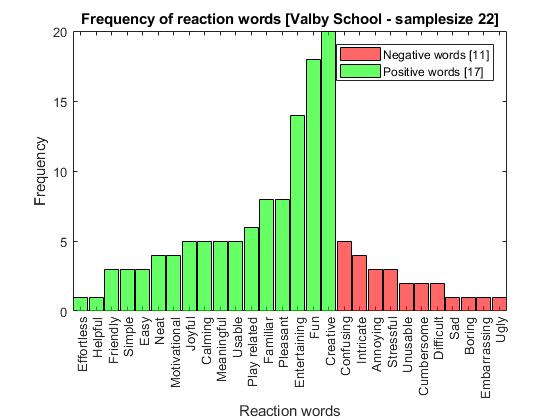
\includegraphics[width=0.9\linewidth]{figure/Evaluation/histValby}
	\label{fig:valbyTest}
	\caption{Shows frequency of selected reaction words, from the test. The bin color (red or green) divides the words in negative(red) and positive(green) }
	
\end{figure}

This suggests, that the reaction towards the usage of the tool is mostly positive.  As so, it suggests that our design requirements have been fulfilled in terms of inducing Positive emotions – in terms of a positive reaction towards the tool. However, as some negative reaction words have been selected, the deign requirement of not inducing negative emotions, cannot be stated as fully fulfilled, however as stated the overall reaction distribution suggest that, predominantly positive emotions are induced with the usage of the tool, as so, the design requirements main intentions can be said to be fulfilled. 


% LITTERATURLISTE
%\addcontentsline{toc}{chapter}{Litteratur}
%\input{include/backmatter/Litteraturliste}
\bibliography{include/backmatter/bibliography}

\begin{appendices}
\section{Initial interviews}\label{sec:initialInterviews}
	\subsection{Teacher Interview}
		\begin{itemize}
		\item[-] Educational level of the teacher 
		\item[-] Describe a typical class + homework
		\item[-] Which areas withing music is taught (theory, instruments, genres etc.)
		\item[-] Tools and materials(Digital as well as analog, iPads, apps, books, instruments, syntesizers and the incorporation in the class)
		\item[-] Methods used (Didaktiske model)
		\item[-] Shortcommings and keeping the engagement of the children
		\item[-] Gamification in the classroom
		\item[-] Difference in lectures from grade to grade
		\item[-] Which role the teacher plays, if they're active role or more passive
		\end{itemize}
\end{appendices}

\end{document}
